\section{Data}

\subsection{Raw Data}

We use play-by-play from basketball referenece

% TODO: add citations
Downloaded from Kaggle [citation], scraped using [citation].

We clean and aggregate the data. One-hot encode columns corresponding to game events.

For example, col for jump shot, hook shot, dunk current score for each team, time left, etc.

Full list of columns given in \autoref{tbl:list-of-columns}.

This data is fed into the neural network described in the next section.

\begin{figure}
	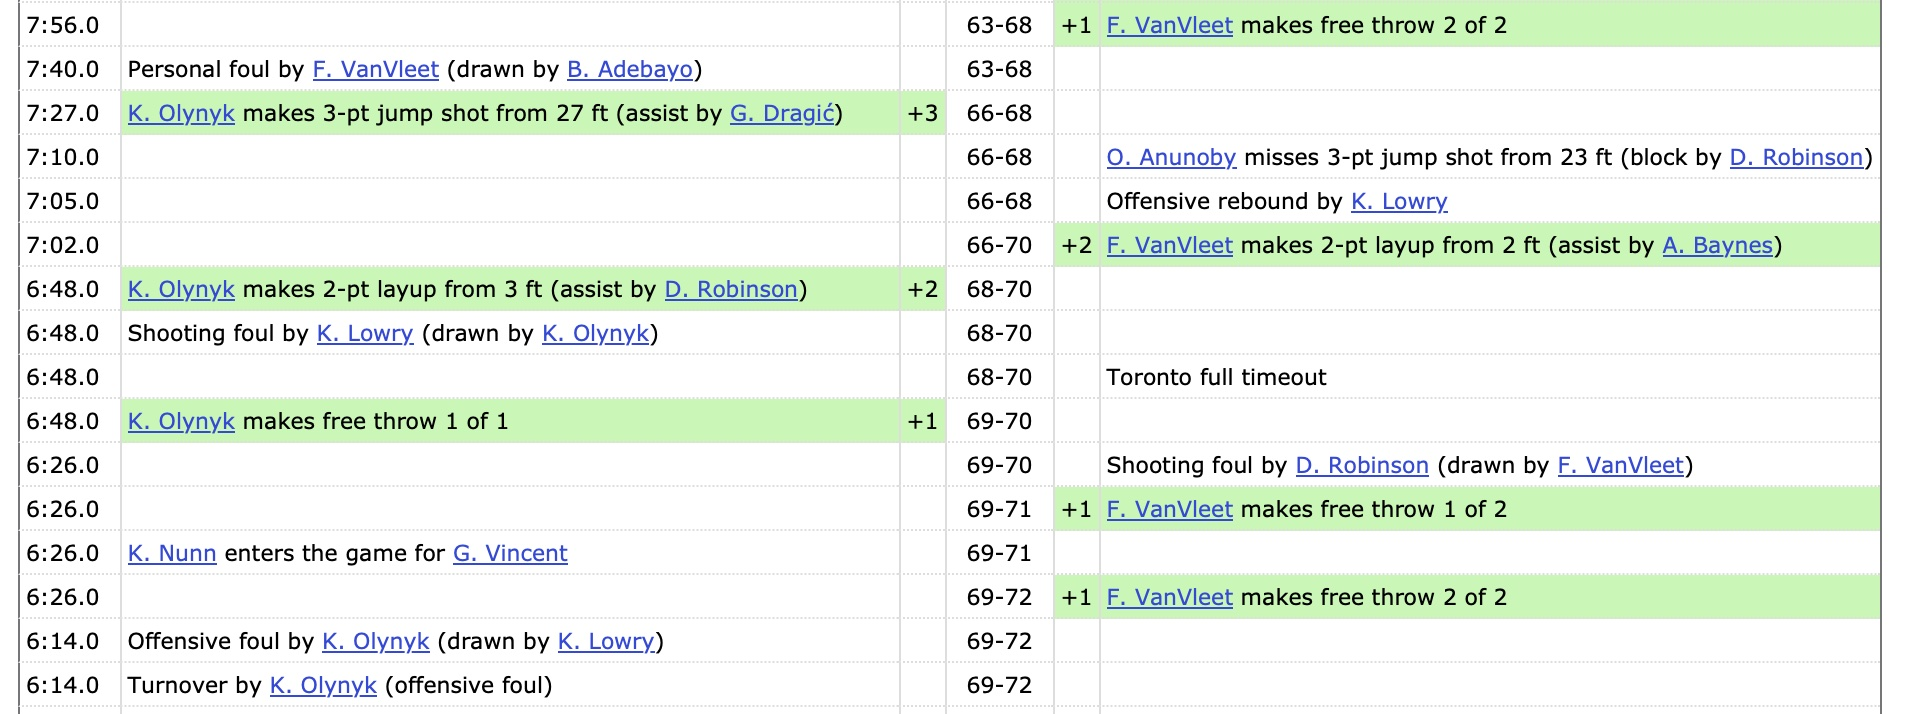
\includegraphics[width = .8 \textwidth]{figures/bbref-pbp.jpg}
	\caption{Example play-by-play data as seen on BasetballReference.com.}
\end{figure}

\begin{table}
	% TODO: make this table
	\caption{The full list of the 69 columns in our data set.}
	\label{tbl:list-of-columns}
\end{table}

\begin{table}
	\centering
	\begin{tabular}{rl}
		\hline
		Event Type  & $n$     \\
		\hline
		Total       & 3040524 \\
		Shots       & 1144001 \\
		Rebounds    & 690893  \\
		Free Throws & 302084  \\
		Fouls       & 275409  \\
		Jumpballs   & 275409  \\
		Turnovers   & 187496  \\
		Violations  & 10884   \\
		\hline
	\end{tabular}
	\caption{Number of events by event type.}
\end{table}

\begin{figure}[h]
	% Created by tikzDevice version 0.12.4 on 2024-02-25 11:31:45
% !TEX encoding = UTF-8 Unicode
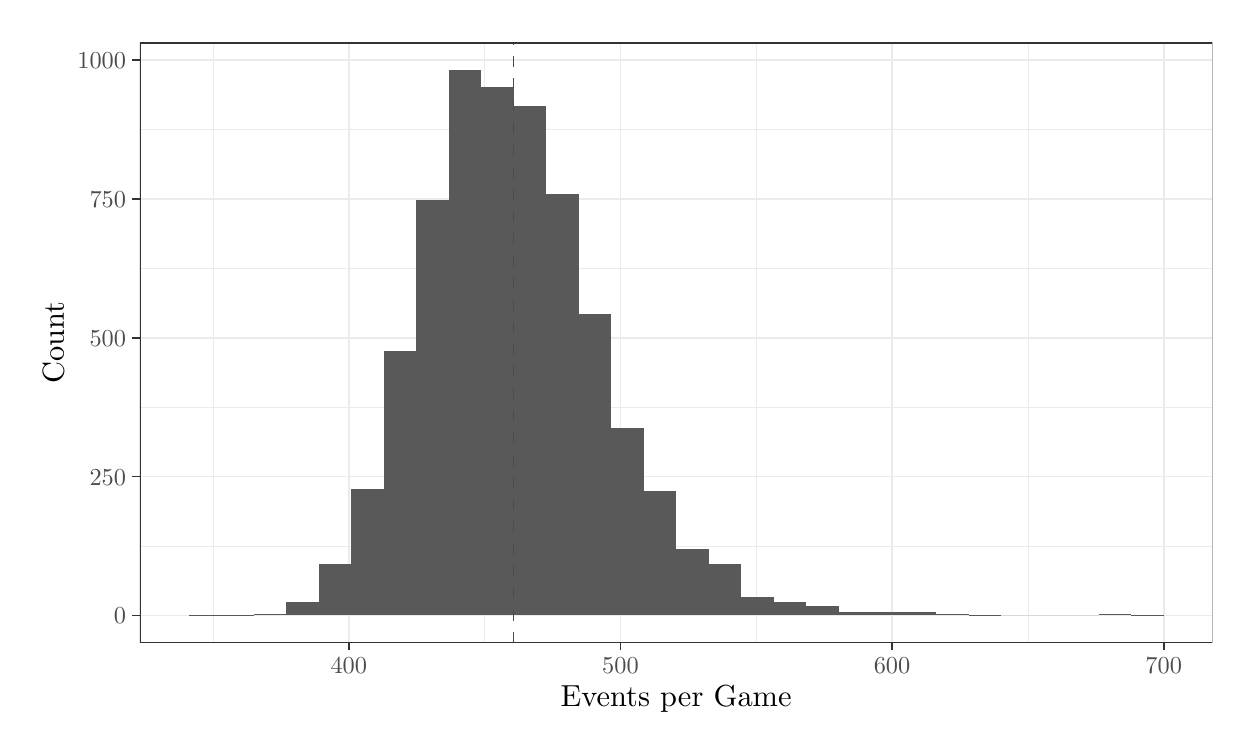
\begin{tikzpicture}[x=1pt,y=1pt]
\definecolor{fillColor}{RGB}{255,255,255}
\path[use as bounding box,fill=fillColor] (0,0) rectangle (433.62,252.94);
\begin{scope}
\path[clip] (  0.00,  0.00) rectangle (433.62,252.94);
\definecolor{drawColor}{RGB}{255,255,255}

\path[draw=drawColor,line width= 0.6pt,line join=round,line cap=round,fill=fillColor] (  0.00,  0.00) rectangle (433.62,252.94);
\end{scope}
\begin{scope}
\path[clip] ( 40.51, 30.69) rectangle (428.12,247.45);
\definecolor{fillColor}{RGB}{255,255,255}

\path[fill=fillColor] ( 40.51, 30.69) rectangle (428.12,247.45);
\definecolor{drawColor}{gray}{0.92}

\path[draw=drawColor,line width= 0.3pt,line join=round] ( 40.51, 65.62) --
	(428.12, 65.62);

\path[draw=drawColor,line width= 0.3pt,line join=round] ( 40.51,115.79) --
	(428.12,115.79);

\path[draw=drawColor,line width= 0.3pt,line join=round] ( 40.51,165.95) --
	(428.12,165.95);

\path[draw=drawColor,line width= 0.3pt,line join=round] ( 40.51,216.12) --
	(428.12,216.12);

\path[draw=drawColor,line width= 0.3pt,line join=round] ( 66.95, 30.69) --
	( 66.95,247.45);

\path[draw=drawColor,line width= 0.3pt,line join=round] (165.11, 30.69) --
	(165.11,247.45);

\path[draw=drawColor,line width= 0.3pt,line join=round] (263.27, 30.69) --
	(263.27,247.45);

\path[draw=drawColor,line width= 0.3pt,line join=round] (361.44, 30.69) --
	(361.44,247.45);

\path[draw=drawColor,line width= 0.6pt,line join=round] ( 40.51, 40.54) --
	(428.12, 40.54);

\path[draw=drawColor,line width= 0.6pt,line join=round] ( 40.51, 90.70) --
	(428.12, 90.70);

\path[draw=drawColor,line width= 0.6pt,line join=round] ( 40.51,140.87) --
	(428.12,140.87);

\path[draw=drawColor,line width= 0.6pt,line join=round] ( 40.51,191.04) --
	(428.12,191.04);

\path[draw=drawColor,line width= 0.6pt,line join=round] ( 40.51,241.20) --
	(428.12,241.20);

\path[draw=drawColor,line width= 0.6pt,line join=round] (116.03, 30.69) --
	(116.03,247.45);

\path[draw=drawColor,line width= 0.6pt,line join=round] (214.19, 30.69) --
	(214.19,247.45);

\path[draw=drawColor,line width= 0.6pt,line join=round] (312.35, 30.69) --
	(312.35,247.45);

\path[draw=drawColor,line width= 0.6pt,line join=round] (410.52, 30.69) --
	(410.52,247.45);
\definecolor{fillColor}{gray}{0.35}

\path[fill=fillColor] ( 58.13, 40.54) rectangle ( 69.87, 40.74);

\path[fill=fillColor] ( 69.87, 40.54) rectangle ( 81.62, 40.74);

\path[fill=fillColor] ( 81.62, 40.54) rectangle ( 93.37, 40.94);

\path[fill=fillColor] ( 93.37, 40.54) rectangle (105.11, 45.35);

\path[fill=fillColor] (105.11, 40.54) rectangle (116.86, 59.20);

\path[fill=fillColor] (116.86, 40.54) rectangle (128.60, 86.29);

\path[fill=fillColor] (128.60, 40.54) rectangle (140.35,136.06);

\path[fill=fillColor] (140.35, 40.54) rectangle (152.09,190.64);

\path[fill=fillColor] (152.09, 40.54) rectangle (163.84,237.59);

\path[fill=fillColor] (163.84, 40.54) rectangle (175.59,231.37);

\path[fill=fillColor] (175.59, 40.54) rectangle (187.33,224.75);

\path[fill=fillColor] (187.33, 40.54) rectangle (199.08,192.84);

\path[fill=fillColor] (199.08, 40.54) rectangle (210.82,149.50);

\path[fill=fillColor] (210.82, 40.54) rectangle (222.57,108.16);

\path[fill=fillColor] (222.57, 40.54) rectangle (234.32, 85.49);

\path[fill=fillColor] (234.32, 40.54) rectangle (246.06, 64.62);

\path[fill=fillColor] (246.06, 40.54) rectangle (257.81, 59.20);

\path[fill=fillColor] (257.81, 40.54) rectangle (269.55, 47.36);

\path[fill=fillColor] (269.55, 40.54) rectangle (281.30, 45.35);

\path[fill=fillColor] (281.30, 40.54) rectangle (293.04, 43.95);

\path[fill=fillColor] (293.04, 40.54) rectangle (304.79, 41.94);

\path[fill=fillColor] (304.79, 40.54) rectangle (316.54, 41.74);

\path[fill=fillColor] (316.54, 40.54) rectangle (328.28, 41.74);

\path[fill=fillColor] (328.28, 40.54) rectangle (340.03, 40.94);

\path[fill=fillColor] (340.03, 40.54) rectangle (351.77, 40.74);

\path[fill=fillColor] (351.77, 40.54) rectangle (363.52, 40.54);

\path[fill=fillColor] (363.52, 40.54) rectangle (375.26, 40.54);

\path[fill=fillColor] (375.26, 40.54) rectangle (387.01, 40.54);

\path[fill=fillColor] (387.01, 40.54) rectangle (398.76, 40.94);

\path[fill=fillColor] (398.76, 40.54) rectangle (410.50, 40.74);
\definecolor{drawColor}{RGB}{255,0,0}

\path[draw=drawColor,line width= 0.6pt,dash pattern=on 4pt off 4pt ,line join=round] (175.60, 30.69) -- (175.60,247.45);
\definecolor{drawColor}{gray}{0.20}

\path[draw=drawColor,line width= 0.6pt,line join=round,line cap=round] ( 40.51, 30.69) rectangle (428.12,247.45);
\end{scope}
\begin{scope}
\path[clip] (  0.00,  0.00) rectangle (433.62,252.94);
\definecolor{drawColor}{gray}{0.30}

\node[text=drawColor,anchor=base east,inner sep=0pt, outer sep=0pt, scale=  0.88] at ( 35.56, 37.51) {0};

\node[text=drawColor,anchor=base east,inner sep=0pt, outer sep=0pt, scale=  0.88] at ( 35.56, 87.67) {250};

\node[text=drawColor,anchor=base east,inner sep=0pt, outer sep=0pt, scale=  0.88] at ( 35.56,137.84) {500};

\node[text=drawColor,anchor=base east,inner sep=0pt, outer sep=0pt, scale=  0.88] at ( 35.56,188.01) {750};

\node[text=drawColor,anchor=base east,inner sep=0pt, outer sep=0pt, scale=  0.88] at ( 35.56,238.17) {1000};
\end{scope}
\begin{scope}
\path[clip] (  0.00,  0.00) rectangle (433.62,252.94);
\definecolor{drawColor}{gray}{0.20}

\path[draw=drawColor,line width= 0.6pt,line join=round] ( 37.76, 40.54) --
	( 40.51, 40.54);

\path[draw=drawColor,line width= 0.6pt,line join=round] ( 37.76, 90.70) --
	( 40.51, 90.70);

\path[draw=drawColor,line width= 0.6pt,line join=round] ( 37.76,140.87) --
	( 40.51,140.87);

\path[draw=drawColor,line width= 0.6pt,line join=round] ( 37.76,191.04) --
	( 40.51,191.04);

\path[draw=drawColor,line width= 0.6pt,line join=round] ( 37.76,241.20) --
	( 40.51,241.20);
\end{scope}
\begin{scope}
\path[clip] (  0.00,  0.00) rectangle (433.62,252.94);
\definecolor{drawColor}{gray}{0.20}

\path[draw=drawColor,line width= 0.6pt,line join=round] (116.03, 27.94) --
	(116.03, 30.69);

\path[draw=drawColor,line width= 0.6pt,line join=round] (214.19, 27.94) --
	(214.19, 30.69);

\path[draw=drawColor,line width= 0.6pt,line join=round] (312.35, 27.94) --
	(312.35, 30.69);

\path[draw=drawColor,line width= 0.6pt,line join=round] (410.52, 27.94) --
	(410.52, 30.69);
\end{scope}
\begin{scope}
\path[clip] (  0.00,  0.00) rectangle (433.62,252.94);
\definecolor{drawColor}{gray}{0.30}

\node[text=drawColor,anchor=base,inner sep=0pt, outer sep=0pt, scale=  0.88] at (116.03, 19.68) {400};

\node[text=drawColor,anchor=base,inner sep=0pt, outer sep=0pt, scale=  0.88] at (214.19, 19.68) {500};

\node[text=drawColor,anchor=base,inner sep=0pt, outer sep=0pt, scale=  0.88] at (312.35, 19.68) {600};

\node[text=drawColor,anchor=base,inner sep=0pt, outer sep=0pt, scale=  0.88] at (410.52, 19.68) {700};
\end{scope}
\begin{scope}
\path[clip] (  0.00,  0.00) rectangle (433.62,252.94);
\definecolor{drawColor}{RGB}{0,0,0}

\node[text=drawColor,anchor=base,inner sep=0pt, outer sep=0pt, scale=  1.10] at (234.32,  7.64) {Events per Game};
\end{scope}
\begin{scope}
\path[clip] (  0.00,  0.00) rectangle (433.62,252.94);
\definecolor{drawColor}{RGB}{0,0,0}

\node[text=drawColor,rotate= 90.00,anchor=base,inner sep=0pt, outer sep=0pt, scale=  1.10] at ( 13.08,139.07) {Count};
\end{scope}
\end{tikzpicture}

	\caption{The distribution of number of events per game with the mean (461) shown in red.}
\end{figure}

\begin{figure}[h]
	% Created by tikzDevice version 0.12.4 on 2024-02-25 11:31:46
% !TEX encoding = UTF-8 Unicode
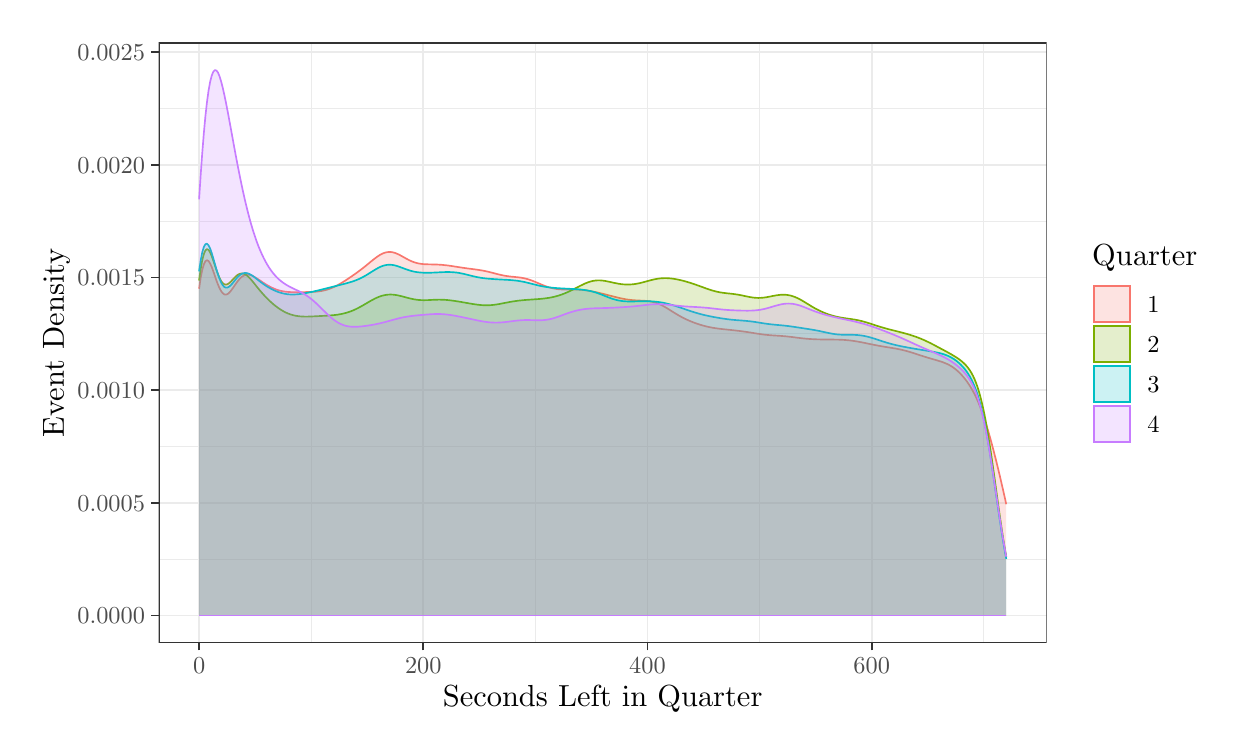
\begin{tikzpicture}[x=1pt,y=1pt]
\definecolor{fillColor}{RGB}{255,255,255}
\path[use as bounding box,fill=fillColor] (0,0) rectangle (433.62,252.94);
\begin{scope}
\path[clip] (  0.00,  0.00) rectangle (433.62,252.94);
\definecolor{drawColor}{RGB}{255,255,255}

\path[draw=drawColor,line width= 0.6pt,line join=round,line cap=round,fill=fillColor] (  0.00,  0.00) rectangle (433.62,252.94);
\end{scope}
\begin{scope}
\path[clip] ( 47.35, 30.69) rectangle (368.18,247.45);
\definecolor{fillColor}{RGB}{255,255,255}

\path[fill=fillColor] ( 47.35, 30.69) rectangle (368.18,247.45);
\definecolor{drawColor}{gray}{0.92}

\path[draw=drawColor,line width= 0.3pt,line join=round] ( 47.35, 60.90) --
	(368.18, 60.90);

\path[draw=drawColor,line width= 0.3pt,line join=round] ( 47.35,101.62) --
	(368.18,101.62);

\path[draw=drawColor,line width= 0.3pt,line join=round] ( 47.35,142.34) --
	(368.18,142.34);

\path[draw=drawColor,line width= 0.3pt,line join=round] ( 47.35,183.06) --
	(368.18,183.06);

\path[draw=drawColor,line width= 0.3pt,line join=round] ( 47.35,223.77) --
	(368.18,223.77);

\path[draw=drawColor,line width= 0.3pt,line join=round] (102.44, 30.69) --
	(102.44,247.45);

\path[draw=drawColor,line width= 0.3pt,line join=round] (183.46, 30.69) --
	(183.46,247.45);

\path[draw=drawColor,line width= 0.3pt,line join=round] (264.48, 30.69) --
	(264.48,247.45);

\path[draw=drawColor,line width= 0.3pt,line join=round] (345.49, 30.69) --
	(345.49,247.45);

\path[draw=drawColor,line width= 0.6pt,line join=round] ( 47.35, 40.54) --
	(368.18, 40.54);

\path[draw=drawColor,line width= 0.6pt,line join=round] ( 47.35, 81.26) --
	(368.18, 81.26);

\path[draw=drawColor,line width= 0.6pt,line join=round] ( 47.35,121.98) --
	(368.18,121.98);

\path[draw=drawColor,line width= 0.6pt,line join=round] ( 47.35,162.70) --
	(368.18,162.70);

\path[draw=drawColor,line width= 0.6pt,line join=round] ( 47.35,203.42) --
	(368.18,203.42);

\path[draw=drawColor,line width= 0.6pt,line join=round] ( 47.35,244.13) --
	(368.18,244.13);

\path[draw=drawColor,line width= 0.6pt,line join=round] ( 61.94, 30.69) --
	( 61.94,247.45);

\path[draw=drawColor,line width= 0.6pt,line join=round] (142.95, 30.69) --
	(142.95,247.45);

\path[draw=drawColor,line width= 0.6pt,line join=round] (223.97, 30.69) --
	(223.97,247.45);

\path[draw=drawColor,line width= 0.6pt,line join=round] (304.99, 30.69) --
	(304.99,247.45);
\definecolor{fillColor}{RGB}{248,118,109}

\path[fill=fillColor,fill opacity=0.20] ( 61.94,158.59) --
	( 62.51,162.53) --
	( 63.08,165.42) --
	( 63.65,167.41) --
	( 64.22,168.55) --
	( 64.79,168.91) --
	( 65.36,168.60) --
	( 65.93,167.74) --
	( 66.50,166.47) --
	( 67.07,164.92) --
	( 67.64,163.24) --
	( 68.21,161.58) --
	( 68.79,160.06) --
	( 69.36,158.75) --
	( 69.93,157.71) --
	( 70.50,156.98) --
	( 71.07,156.56) --
	( 71.64,156.46) --
	( 72.21,156.67) --
	( 72.78,157.12) --
	( 73.35,157.76) --
	( 73.92,158.51) --
	( 74.49,159.33) --
	( 75.06,160.17) --
	( 75.63,160.98) --
	( 76.21,161.73) --
	( 76.78,162.38) --
	( 77.35,162.89) --
	( 77.92,163.28) --
	( 78.49,163.54) --
	( 79.06,163.67) --
	( 79.63,163.69) --
	( 80.20,163.61) --
	( 80.77,163.44) --
	( 81.34,163.20) --
	( 81.91,162.89) --
	( 82.48,162.55) --
	( 83.05,162.19) --
	( 83.62,161.80) --
	( 84.20,161.42) --
	( 84.77,161.03) --
	( 85.34,160.65) --
	( 85.91,160.29) --
	( 86.48,159.94) --
	( 87.05,159.61) --
	( 87.62,159.31) --
	( 88.19,159.02) --
	( 88.76,158.76) --
	( 89.33,158.52) --
	( 89.90,158.30) --
	( 90.47,158.11) --
	( 91.04,157.95) --
	( 91.62,157.81) --
	( 92.19,157.70) --
	( 92.76,157.60) --
	( 93.33,157.52) --
	( 93.90,157.46) --
	( 94.47,157.42) --
	( 95.04,157.39) --
	( 95.61,157.37) --
	( 96.18,157.36) --
	( 96.75,157.36) --
	( 97.32,157.36) --
	( 97.89,157.36) --
	( 98.46,157.37) --
	( 99.04,157.38) --
	( 99.61,157.38) --
	(100.18,157.39) --
	(100.75,157.40) --
	(101.32,157.41) --
	(101.89,157.43) --
	(102.46,157.44) --
	(103.03,157.47) --
	(103.60,157.50) --
	(104.17,157.54) --
	(104.74,157.60) --
	(105.31,157.67) --
	(105.88,157.75) --
	(106.46,157.85) --
	(107.03,157.97) --
	(107.60,158.11) --
	(108.17,158.27) --
	(108.74,158.46) --
	(109.31,158.66) --
	(109.88,158.89) --
	(110.45,159.13) --
	(111.02,159.40) --
	(111.59,159.69) --
	(112.16,159.99) --
	(112.73,160.31) --
	(113.30,160.64) --
	(113.88,160.99) --
	(114.45,161.34) --
	(115.02,161.71) --
	(115.59,162.08) --
	(116.16,162.46) --
	(116.73,162.85) --
	(117.30,163.24) --
	(117.87,163.64) --
	(118.44,164.04) --
	(119.01,164.46) --
	(119.58,164.88) --
	(120.15,165.30) --
	(120.72,165.74) --
	(121.30,166.18) --
	(121.87,166.64) --
	(122.44,167.10) --
	(123.01,167.57) --
	(123.58,168.04) --
	(124.15,168.51) --
	(124.72,168.97) --
	(125.29,169.42) --
	(125.86,169.85) --
	(126.43,170.26) --
	(127.00,170.64) --
	(127.57,170.98) --
	(128.14,171.27) --
	(128.72,171.51) --
	(129.29,171.69) --
	(129.86,171.81) --
	(130.43,171.88) --
	(131.00,171.88) --
	(131.57,171.83) --
	(132.14,171.71) --
	(132.71,171.55) --
	(133.28,171.33) --
	(133.85,171.08) --
	(134.42,170.80) --
	(134.99,170.49) --
	(135.56,170.17) --
	(136.14,169.85) --
	(136.71,169.53) --
	(137.28,169.22) --
	(137.85,168.93) --
	(138.42,168.66) --
	(138.99,168.42) --
	(139.56,168.21) --
	(140.13,168.02) --
	(140.70,167.87) --
	(141.27,167.74) --
	(141.84,167.64) --
	(142.41,167.56) --
	(142.98,167.50) --
	(143.56,167.46) --
	(144.13,167.44) --
	(144.70,167.42) --
	(145.27,167.40) --
	(145.84,167.39) --
	(146.41,167.38) --
	(146.98,167.37) --
	(147.55,167.35) --
	(148.12,167.33) --
	(148.69,167.30) --
	(149.26,167.26) --
	(149.83,167.22) --
	(150.40,167.16) --
	(150.98,167.10) --
	(151.55,167.04) --
	(152.12,166.96) --
	(152.69,166.88) --
	(153.26,166.80) --
	(153.83,166.71) --
	(154.40,166.62) --
	(154.97,166.53) --
	(155.54,166.44) --
	(156.11,166.35) --
	(156.68,166.27) --
	(157.25,166.18) --
	(157.82,166.10) --
	(158.39,166.02) --
	(158.97,165.94) --
	(159.54,165.86) --
	(160.11,165.79) --
	(160.68,165.72) --
	(161.25,165.64) --
	(161.82,165.57) --
	(162.39,165.49) --
	(162.96,165.40) --
	(163.53,165.31) --
	(164.10,165.22) --
	(164.67,165.11) --
	(165.24,165.00) --
	(165.81,164.88) --
	(166.39,164.75) --
	(166.96,164.61) --
	(167.53,164.46) --
	(168.10,164.32) --
	(168.67,164.17) --
	(169.24,164.02) --
	(169.81,163.87) --
	(170.38,163.73) --
	(170.95,163.60) --
	(171.52,163.47) --
	(172.09,163.36) --
	(172.66,163.26) --
	(173.23,163.17) --
	(173.81,163.09) --
	(174.38,163.02) --
	(174.95,162.96) --
	(175.52,162.91) --
	(176.09,162.85) --
	(176.66,162.79) --
	(177.23,162.73) --
	(177.80,162.66) --
	(178.37,162.58) --
	(178.94,162.48) --
	(179.51,162.36) --
	(180.08,162.23) --
	(180.65,162.07) --
	(181.23,161.89) --
	(181.80,161.70) --
	(182.37,161.49) --
	(182.94,161.26) --
	(183.51,161.03) --
	(184.08,160.79) --
	(184.65,160.54) --
	(185.22,160.30) --
	(185.79,160.06) --
	(186.36,159.83) --
	(186.93,159.61) --
	(187.50,159.40) --
	(188.07,159.21) --
	(188.65,159.04) --
	(189.22,158.88) --
	(189.79,158.75) --
	(190.36,158.64) --
	(190.93,158.54) --
	(191.50,158.46) --
	(192.07,158.40) --
	(192.64,158.36) --
	(193.21,158.33) --
	(193.78,158.31) --
	(194.35,158.31) --
	(194.92,158.31) --
	(195.49,158.31) --
	(196.07,158.31) --
	(196.64,158.32) --
	(197.21,158.32) --
	(197.78,158.32) --
	(198.35,158.30) --
	(198.92,158.28) --
	(199.49,158.25) --
	(200.06,158.21) --
	(200.63,158.16) --
	(201.20,158.09) --
	(201.77,158.02) --
	(202.34,157.94) --
	(202.91,157.84) --
	(203.49,157.74) --
	(204.06,157.63) --
	(204.63,157.51) --
	(205.20,157.39) --
	(205.77,157.26) --
	(206.34,157.13) --
	(206.91,156.99) --
	(207.48,156.86) --
	(208.05,156.72) --
	(208.62,156.57) --
	(209.19,156.43) --
	(209.76,156.28) --
	(210.33,156.14) --
	(210.91,155.99) --
	(211.48,155.84) --
	(212.05,155.70) --
	(212.62,155.55) --
	(213.19,155.41) --
	(213.76,155.28) --
	(214.33,155.15) --
	(214.90,155.03) --
	(215.47,154.92) --
	(216.04,154.81) --
	(216.61,154.72) --
	(217.18,154.64) --
	(217.75,154.57) --
	(218.33,154.51) --
	(218.90,154.46) --
	(219.47,154.42) --
	(220.04,154.39) --
	(220.61,154.36) --
	(221.18,154.33) --
	(221.75,154.31) --
	(222.32,154.29) --
	(222.89,154.25) --
	(223.46,154.21) --
	(224.03,154.15) --
	(224.60,154.08) --
	(225.17,153.98) --
	(225.75,153.87) --
	(226.32,153.73) --
	(226.89,153.56) --
	(227.46,153.36) --
	(228.03,153.13) --
	(228.60,152.88) --
	(229.17,152.60) --
	(229.74,152.30) --
	(230.31,151.98) --
	(230.88,151.65) --
	(231.45,151.30) --
	(232.02,150.94) --
	(232.59,150.58) --
	(233.16,150.22) --
	(233.74,149.87) --
	(234.31,149.52) --
	(234.88,149.18) --
	(235.45,148.85) --
	(236.02,148.53) --
	(236.59,148.22) --
	(237.16,147.93) --
	(237.73,147.65) --
	(238.30,147.39) --
	(238.87,147.13) --
	(239.44,146.89) --
	(240.01,146.66) --
	(240.58,146.43) --
	(241.16,146.22) --
	(241.73,146.02) --
	(242.30,145.82) --
	(242.87,145.64) --
	(243.44,145.47) --
	(244.01,145.30) --
	(244.58,145.15) --
	(245.15,145.00) --
	(245.72,144.87) --
	(246.29,144.74) --
	(246.86,144.63) --
	(247.43,144.52) --
	(248.00,144.43) --
	(248.58,144.34) --
	(249.15,144.26) --
	(249.72,144.18) --
	(250.29,144.11) --
	(250.86,144.04) --
	(251.43,143.98) --
	(252.00,143.92) --
	(252.57,143.86) --
	(253.14,143.80) --
	(253.71,143.74) --
	(254.28,143.68) --
	(254.85,143.62) --
	(255.42,143.56) --
	(256.00,143.49) --
	(256.57,143.42) --
	(257.14,143.35) --
	(257.71,143.28) --
	(258.28,143.20) --
	(258.85,143.12) --
	(259.42,143.04) --
	(259.99,142.96) --
	(260.56,142.87) --
	(261.13,142.78) --
	(261.70,142.69) --
	(262.27,142.60) --
	(262.84,142.50) --
	(263.42,142.41) --
	(263.99,142.33) --
	(264.56,142.24) --
	(265.13,142.16) --
	(265.70,142.08) --
	(266.27,142.01) --
	(266.84,141.95) --
	(267.41,141.89) --
	(267.98,141.84) --
	(268.55,141.79) --
	(269.12,141.75) --
	(269.69,141.71) --
	(270.26,141.68) --
	(270.84,141.64) --
	(271.41,141.60) --
	(271.98,141.57) --
	(272.55,141.52) --
	(273.12,141.48) --
	(273.69,141.43) --
	(274.26,141.37) --
	(274.83,141.31) --
	(275.40,141.25) --
	(275.97,141.18) --
	(276.54,141.11) --
	(277.11,141.04) --
	(277.68,140.96) --
	(278.26,140.89) --
	(278.83,140.82) --
	(279.40,140.75) --
	(279.97,140.69) --
	(280.54,140.63) --
	(281.11,140.57) --
	(281.68,140.52) --
	(282.25,140.47) --
	(282.82,140.43) --
	(283.39,140.40) --
	(283.96,140.37) --
	(284.53,140.35) --
	(285.10,140.32) --
	(285.68,140.31) --
	(286.25,140.29) --
	(286.82,140.28) --
	(287.39,140.27) --
	(287.96,140.26) --
	(288.53,140.26) --
	(289.10,140.25) --
	(289.67,140.25) --
	(290.24,140.25) --
	(290.81,140.24) --
	(291.38,140.23) --
	(291.95,140.23) --
	(292.52,140.21) --
	(293.10,140.20) --
	(293.67,140.18) --
	(294.24,140.15) --
	(294.81,140.12) --
	(295.38,140.08) --
	(295.95,140.03) --
	(296.52,139.98) --
	(297.09,139.92) --
	(297.66,139.85) --
	(298.23,139.77) --
	(298.80,139.69) --
	(299.37,139.60) --
	(299.94,139.50) --
	(300.52,139.40) --
	(301.09,139.29) --
	(301.66,139.18) --
	(302.23,139.07) --
	(302.80,138.95) --
	(303.37,138.83) --
	(303.94,138.71) --
	(304.51,138.59) --
	(305.08,138.48) --
	(305.65,138.36) --
	(306.22,138.25) --
	(306.79,138.14) --
	(307.36,138.03) --
	(307.93,137.93) --
	(308.51,137.83) --
	(309.08,137.73) --
	(309.65,137.63) --
	(310.22,137.54) --
	(310.79,137.45) --
	(311.36,137.36) --
	(311.93,137.27) --
	(312.50,137.17) --
	(313.07,137.08) --
	(313.64,136.98) --
	(314.21,136.87) --
	(314.78,136.76) --
	(315.35,136.64) --
	(315.93,136.51) --
	(316.50,136.37) --
	(317.07,136.23) --
	(317.64,136.08) --
	(318.21,135.92) --
	(318.78,135.75) --
	(319.35,135.58) --
	(319.92,135.40) --
	(320.49,135.22) --
	(321.06,135.03) --
	(321.63,134.84) --
	(322.20,134.66) --
	(322.77,134.47) --
	(323.35,134.29) --
	(323.92,134.11) --
	(324.49,133.93) --
	(325.06,133.75) --
	(325.63,133.58) --
	(326.20,133.41) --
	(326.77,133.25) --
	(327.34,133.08) --
	(327.91,132.92) --
	(328.48,132.75) --
	(329.05,132.58) --
	(329.62,132.40) --
	(330.19,132.22) --
	(330.77,132.02) --
	(331.34,131.80) --
	(331.91,131.56) --
	(332.48,131.30) --
	(333.05,131.01) --
	(333.62,130.68) --
	(334.19,130.33) --
	(334.76,129.93) --
	(335.33,129.48) --
	(335.90,129.00) --
	(336.47,128.47) --
	(337.04,127.91) --
	(337.61,127.29) --
	(338.19,126.63) --
	(338.76,125.93) --
	(339.33,125.17) --
	(339.90,124.36) --
	(340.47,123.48) --
	(341.04,122.54) --
	(341.61,121.53) --
	(342.18,120.45) --
	(342.75,119.28) --
	(343.32,118.02) --
	(343.89,116.66) --
	(344.46,115.18) --
	(345.03,113.61) --
	(345.61,111.94) --
	(346.18,110.17) --
	(346.75,108.31) --
	(347.32,106.37) --
	(347.89,104.35) --
	(348.46,102.25) --
	(349.03,100.09) --
	(349.60, 97.86) --
	(350.17, 95.58) --
	(350.74, 93.24) --
	(351.31, 90.85) --
	(351.88, 88.40) --
	(352.45, 85.90) --
	(353.03, 83.35) --
	(353.60, 80.74) --
	(353.60, 40.54) --
	(353.03, 40.54) --
	(352.45, 40.54) --
	(351.88, 40.54) --
	(351.31, 40.54) --
	(350.74, 40.54) --
	(350.17, 40.54) --
	(349.60, 40.54) --
	(349.03, 40.54) --
	(348.46, 40.54) --
	(347.89, 40.54) --
	(347.32, 40.54) --
	(346.75, 40.54) --
	(346.18, 40.54) --
	(345.61, 40.54) --
	(345.03, 40.54) --
	(344.46, 40.54) --
	(343.89, 40.54) --
	(343.32, 40.54) --
	(342.75, 40.54) --
	(342.18, 40.54) --
	(341.61, 40.54) --
	(341.04, 40.54) --
	(340.47, 40.54) --
	(339.90, 40.54) --
	(339.33, 40.54) --
	(338.76, 40.54) --
	(338.19, 40.54) --
	(337.61, 40.54) --
	(337.04, 40.54) --
	(336.47, 40.54) --
	(335.90, 40.54) --
	(335.33, 40.54) --
	(334.76, 40.54) --
	(334.19, 40.54) --
	(333.62, 40.54) --
	(333.05, 40.54) --
	(332.48, 40.54) --
	(331.91, 40.54) --
	(331.34, 40.54) --
	(330.77, 40.54) --
	(330.19, 40.54) --
	(329.62, 40.54) --
	(329.05, 40.54) --
	(328.48, 40.54) --
	(327.91, 40.54) --
	(327.34, 40.54) --
	(326.77, 40.54) --
	(326.20, 40.54) --
	(325.63, 40.54) --
	(325.06, 40.54) --
	(324.49, 40.54) --
	(323.92, 40.54) --
	(323.35, 40.54) --
	(322.77, 40.54) --
	(322.20, 40.54) --
	(321.63, 40.54) --
	(321.06, 40.54) --
	(320.49, 40.54) --
	(319.92, 40.54) --
	(319.35, 40.54) --
	(318.78, 40.54) --
	(318.21, 40.54) --
	(317.64, 40.54) --
	(317.07, 40.54) --
	(316.50, 40.54) --
	(315.93, 40.54) --
	(315.35, 40.54) --
	(314.78, 40.54) --
	(314.21, 40.54) --
	(313.64, 40.54) --
	(313.07, 40.54) --
	(312.50, 40.54) --
	(311.93, 40.54) --
	(311.36, 40.54) --
	(310.79, 40.54) --
	(310.22, 40.54) --
	(309.65, 40.54) --
	(309.08, 40.54) --
	(308.51, 40.54) --
	(307.93, 40.54) --
	(307.36, 40.54) --
	(306.79, 40.54) --
	(306.22, 40.54) --
	(305.65, 40.54) --
	(305.08, 40.54) --
	(304.51, 40.54) --
	(303.94, 40.54) --
	(303.37, 40.54) --
	(302.80, 40.54) --
	(302.23, 40.54) --
	(301.66, 40.54) --
	(301.09, 40.54) --
	(300.52, 40.54) --
	(299.94, 40.54) --
	(299.37, 40.54) --
	(298.80, 40.54) --
	(298.23, 40.54) --
	(297.66, 40.54) --
	(297.09, 40.54) --
	(296.52, 40.54) --
	(295.95, 40.54) --
	(295.38, 40.54) --
	(294.81, 40.54) --
	(294.24, 40.54) --
	(293.67, 40.54) --
	(293.10, 40.54) --
	(292.52, 40.54) --
	(291.95, 40.54) --
	(291.38, 40.54) --
	(290.81, 40.54) --
	(290.24, 40.54) --
	(289.67, 40.54) --
	(289.10, 40.54) --
	(288.53, 40.54) --
	(287.96, 40.54) --
	(287.39, 40.54) --
	(286.82, 40.54) --
	(286.25, 40.54) --
	(285.68, 40.54) --
	(285.10, 40.54) --
	(284.53, 40.54) --
	(283.96, 40.54) --
	(283.39, 40.54) --
	(282.82, 40.54) --
	(282.25, 40.54) --
	(281.68, 40.54) --
	(281.11, 40.54) --
	(280.54, 40.54) --
	(279.97, 40.54) --
	(279.40, 40.54) --
	(278.83, 40.54) --
	(278.26, 40.54) --
	(277.68, 40.54) --
	(277.11, 40.54) --
	(276.54, 40.54) --
	(275.97, 40.54) --
	(275.40, 40.54) --
	(274.83, 40.54) --
	(274.26, 40.54) --
	(273.69, 40.54) --
	(273.12, 40.54) --
	(272.55, 40.54) --
	(271.98, 40.54) --
	(271.41, 40.54) --
	(270.84, 40.54) --
	(270.26, 40.54) --
	(269.69, 40.54) --
	(269.12, 40.54) --
	(268.55, 40.54) --
	(267.98, 40.54) --
	(267.41, 40.54) --
	(266.84, 40.54) --
	(266.27, 40.54) --
	(265.70, 40.54) --
	(265.13, 40.54) --
	(264.56, 40.54) --
	(263.99, 40.54) --
	(263.42, 40.54) --
	(262.84, 40.54) --
	(262.27, 40.54) --
	(261.70, 40.54) --
	(261.13, 40.54) --
	(260.56, 40.54) --
	(259.99, 40.54) --
	(259.42, 40.54) --
	(258.85, 40.54) --
	(258.28, 40.54) --
	(257.71, 40.54) --
	(257.14, 40.54) --
	(256.57, 40.54) --
	(256.00, 40.54) --
	(255.42, 40.54) --
	(254.85, 40.54) --
	(254.28, 40.54) --
	(253.71, 40.54) --
	(253.14, 40.54) --
	(252.57, 40.54) --
	(252.00, 40.54) --
	(251.43, 40.54) --
	(250.86, 40.54) --
	(250.29, 40.54) --
	(249.72, 40.54) --
	(249.15, 40.54) --
	(248.58, 40.54) --
	(248.00, 40.54) --
	(247.43, 40.54) --
	(246.86, 40.54) --
	(246.29, 40.54) --
	(245.72, 40.54) --
	(245.15, 40.54) --
	(244.58, 40.54) --
	(244.01, 40.54) --
	(243.44, 40.54) --
	(242.87, 40.54) --
	(242.30, 40.54) --
	(241.73, 40.54) --
	(241.16, 40.54) --
	(240.58, 40.54) --
	(240.01, 40.54) --
	(239.44, 40.54) --
	(238.87, 40.54) --
	(238.30, 40.54) --
	(237.73, 40.54) --
	(237.16, 40.54) --
	(236.59, 40.54) --
	(236.02, 40.54) --
	(235.45, 40.54) --
	(234.88, 40.54) --
	(234.31, 40.54) --
	(233.74, 40.54) --
	(233.16, 40.54) --
	(232.59, 40.54) --
	(232.02, 40.54) --
	(231.45, 40.54) --
	(230.88, 40.54) --
	(230.31, 40.54) --
	(229.74, 40.54) --
	(229.17, 40.54) --
	(228.60, 40.54) --
	(228.03, 40.54) --
	(227.46, 40.54) --
	(226.89, 40.54) --
	(226.32, 40.54) --
	(225.75, 40.54) --
	(225.17, 40.54) --
	(224.60, 40.54) --
	(224.03, 40.54) --
	(223.46, 40.54) --
	(222.89, 40.54) --
	(222.32, 40.54) --
	(221.75, 40.54) --
	(221.18, 40.54) --
	(220.61, 40.54) --
	(220.04, 40.54) --
	(219.47, 40.54) --
	(218.90, 40.54) --
	(218.33, 40.54) --
	(217.75, 40.54) --
	(217.18, 40.54) --
	(216.61, 40.54) --
	(216.04, 40.54) --
	(215.47, 40.54) --
	(214.90, 40.54) --
	(214.33, 40.54) --
	(213.76, 40.54) --
	(213.19, 40.54) --
	(212.62, 40.54) --
	(212.05, 40.54) --
	(211.48, 40.54) --
	(210.91, 40.54) --
	(210.33, 40.54) --
	(209.76, 40.54) --
	(209.19, 40.54) --
	(208.62, 40.54) --
	(208.05, 40.54) --
	(207.48, 40.54) --
	(206.91, 40.54) --
	(206.34, 40.54) --
	(205.77, 40.54) --
	(205.20, 40.54) --
	(204.63, 40.54) --
	(204.06, 40.54) --
	(203.49, 40.54) --
	(202.91, 40.54) --
	(202.34, 40.54) --
	(201.77, 40.54) --
	(201.20, 40.54) --
	(200.63, 40.54) --
	(200.06, 40.54) --
	(199.49, 40.54) --
	(198.92, 40.54) --
	(198.35, 40.54) --
	(197.78, 40.54) --
	(197.21, 40.54) --
	(196.64, 40.54) --
	(196.07, 40.54) --
	(195.49, 40.54) --
	(194.92, 40.54) --
	(194.35, 40.54) --
	(193.78, 40.54) --
	(193.21, 40.54) --
	(192.64, 40.54) --
	(192.07, 40.54) --
	(191.50, 40.54) --
	(190.93, 40.54) --
	(190.36, 40.54) --
	(189.79, 40.54) --
	(189.22, 40.54) --
	(188.65, 40.54) --
	(188.07, 40.54) --
	(187.50, 40.54) --
	(186.93, 40.54) --
	(186.36, 40.54) --
	(185.79, 40.54) --
	(185.22, 40.54) --
	(184.65, 40.54) --
	(184.08, 40.54) --
	(183.51, 40.54) --
	(182.94, 40.54) --
	(182.37, 40.54) --
	(181.80, 40.54) --
	(181.23, 40.54) --
	(180.65, 40.54) --
	(180.08, 40.54) --
	(179.51, 40.54) --
	(178.94, 40.54) --
	(178.37, 40.54) --
	(177.80, 40.54) --
	(177.23, 40.54) --
	(176.66, 40.54) --
	(176.09, 40.54) --
	(175.52, 40.54) --
	(174.95, 40.54) --
	(174.38, 40.54) --
	(173.81, 40.54) --
	(173.23, 40.54) --
	(172.66, 40.54) --
	(172.09, 40.54) --
	(171.52, 40.54) --
	(170.95, 40.54) --
	(170.38, 40.54) --
	(169.81, 40.54) --
	(169.24, 40.54) --
	(168.67, 40.54) --
	(168.10, 40.54) --
	(167.53, 40.54) --
	(166.96, 40.54) --
	(166.39, 40.54) --
	(165.81, 40.54) --
	(165.24, 40.54) --
	(164.67, 40.54) --
	(164.10, 40.54) --
	(163.53, 40.54) --
	(162.96, 40.54) --
	(162.39, 40.54) --
	(161.82, 40.54) --
	(161.25, 40.54) --
	(160.68, 40.54) --
	(160.11, 40.54) --
	(159.54, 40.54) --
	(158.97, 40.54) --
	(158.39, 40.54) --
	(157.82, 40.54) --
	(157.25, 40.54) --
	(156.68, 40.54) --
	(156.11, 40.54) --
	(155.54, 40.54) --
	(154.97, 40.54) --
	(154.40, 40.54) --
	(153.83, 40.54) --
	(153.26, 40.54) --
	(152.69, 40.54) --
	(152.12, 40.54) --
	(151.55, 40.54) --
	(150.98, 40.54) --
	(150.40, 40.54) --
	(149.83, 40.54) --
	(149.26, 40.54) --
	(148.69, 40.54) --
	(148.12, 40.54) --
	(147.55, 40.54) --
	(146.98, 40.54) --
	(146.41, 40.54) --
	(145.84, 40.54) --
	(145.27, 40.54) --
	(144.70, 40.54) --
	(144.13, 40.54) --
	(143.56, 40.54) --
	(142.98, 40.54) --
	(142.41, 40.54) --
	(141.84, 40.54) --
	(141.27, 40.54) --
	(140.70, 40.54) --
	(140.13, 40.54) --
	(139.56, 40.54) --
	(138.99, 40.54) --
	(138.42, 40.54) --
	(137.85, 40.54) --
	(137.28, 40.54) --
	(136.71, 40.54) --
	(136.14, 40.54) --
	(135.56, 40.54) --
	(134.99, 40.54) --
	(134.42, 40.54) --
	(133.85, 40.54) --
	(133.28, 40.54) --
	(132.71, 40.54) --
	(132.14, 40.54) --
	(131.57, 40.54) --
	(131.00, 40.54) --
	(130.43, 40.54) --
	(129.86, 40.54) --
	(129.29, 40.54) --
	(128.72, 40.54) --
	(128.14, 40.54) --
	(127.57, 40.54) --
	(127.00, 40.54) --
	(126.43, 40.54) --
	(125.86, 40.54) --
	(125.29, 40.54) --
	(124.72, 40.54) --
	(124.15, 40.54) --
	(123.58, 40.54) --
	(123.01, 40.54) --
	(122.44, 40.54) --
	(121.87, 40.54) --
	(121.30, 40.54) --
	(120.72, 40.54) --
	(120.15, 40.54) --
	(119.58, 40.54) --
	(119.01, 40.54) --
	(118.44, 40.54) --
	(117.87, 40.54) --
	(117.30, 40.54) --
	(116.73, 40.54) --
	(116.16, 40.54) --
	(115.59, 40.54) --
	(115.02, 40.54) --
	(114.45, 40.54) --
	(113.88, 40.54) --
	(113.30, 40.54) --
	(112.73, 40.54) --
	(112.16, 40.54) --
	(111.59, 40.54) --
	(111.02, 40.54) --
	(110.45, 40.54) --
	(109.88, 40.54) --
	(109.31, 40.54) --
	(108.74, 40.54) --
	(108.17, 40.54) --
	(107.60, 40.54) --
	(107.03, 40.54) --
	(106.46, 40.54) --
	(105.88, 40.54) --
	(105.31, 40.54) --
	(104.74, 40.54) --
	(104.17, 40.54) --
	(103.60, 40.54) --
	(103.03, 40.54) --
	(102.46, 40.54) --
	(101.89, 40.54) --
	(101.32, 40.54) --
	(100.75, 40.54) --
	(100.18, 40.54) --
	( 99.61, 40.54) --
	( 99.04, 40.54) --
	( 98.46, 40.54) --
	( 97.89, 40.54) --
	( 97.32, 40.54) --
	( 96.75, 40.54) --
	( 96.18, 40.54) --
	( 95.61, 40.54) --
	( 95.04, 40.54) --
	( 94.47, 40.54) --
	( 93.90, 40.54) --
	( 93.33, 40.54) --
	( 92.76, 40.54) --
	( 92.19, 40.54) --
	( 91.62, 40.54) --
	( 91.04, 40.54) --
	( 90.47, 40.54) --
	( 89.90, 40.54) --
	( 89.33, 40.54) --
	( 88.76, 40.54) --
	( 88.19, 40.54) --
	( 87.62, 40.54) --
	( 87.05, 40.54) --
	( 86.48, 40.54) --
	( 85.91, 40.54) --
	( 85.34, 40.54) --
	( 84.77, 40.54) --
	( 84.20, 40.54) --
	( 83.62, 40.54) --
	( 83.05, 40.54) --
	( 82.48, 40.54) --
	( 81.91, 40.54) --
	( 81.34, 40.54) --
	( 80.77, 40.54) --
	( 80.20, 40.54) --
	( 79.63, 40.54) --
	( 79.06, 40.54) --
	( 78.49, 40.54) --
	( 77.92, 40.54) --
	( 77.35, 40.54) --
	( 76.78, 40.54) --
	( 76.21, 40.54) --
	( 75.63, 40.54) --
	( 75.06, 40.54) --
	( 74.49, 40.54) --
	( 73.92, 40.54) --
	( 73.35, 40.54) --
	( 72.78, 40.54) --
	( 72.21, 40.54) --
	( 71.64, 40.54) --
	( 71.07, 40.54) --
	( 70.50, 40.54) --
	( 69.93, 40.54) --
	( 69.36, 40.54) --
	( 68.79, 40.54) --
	( 68.21, 40.54) --
	( 67.64, 40.54) --
	( 67.07, 40.54) --
	( 66.50, 40.54) --
	( 65.93, 40.54) --
	( 65.36, 40.54) --
	( 64.79, 40.54) --
	( 64.22, 40.54) --
	( 63.65, 40.54) --
	( 63.08, 40.54) --
	( 62.51, 40.54) --
	( 61.94, 40.54) --
	cycle;
\definecolor{drawColor}{RGB}{248,118,109}

\path[draw=drawColor,line width= 0.6pt,line join=round] ( 61.94,158.59) --
	( 62.51,162.53) --
	( 63.08,165.42) --
	( 63.65,167.41) --
	( 64.22,168.55) --
	( 64.79,168.91) --
	( 65.36,168.60) --
	( 65.93,167.74) --
	( 66.50,166.47) --
	( 67.07,164.92) --
	( 67.64,163.24) --
	( 68.21,161.58) --
	( 68.79,160.06) --
	( 69.36,158.75) --
	( 69.93,157.71) --
	( 70.50,156.98) --
	( 71.07,156.56) --
	( 71.64,156.46) --
	( 72.21,156.67) --
	( 72.78,157.12) --
	( 73.35,157.76) --
	( 73.92,158.51) --
	( 74.49,159.33) --
	( 75.06,160.17) --
	( 75.63,160.98) --
	( 76.21,161.73) --
	( 76.78,162.38) --
	( 77.35,162.89) --
	( 77.92,163.28) --
	( 78.49,163.54) --
	( 79.06,163.67) --
	( 79.63,163.69) --
	( 80.20,163.61) --
	( 80.77,163.44) --
	( 81.34,163.20) --
	( 81.91,162.89) --
	( 82.48,162.55) --
	( 83.05,162.19) --
	( 83.62,161.80) --
	( 84.20,161.42) --
	( 84.77,161.03) --
	( 85.34,160.65) --
	( 85.91,160.29) --
	( 86.48,159.94) --
	( 87.05,159.61) --
	( 87.62,159.31) --
	( 88.19,159.02) --
	( 88.76,158.76) --
	( 89.33,158.52) --
	( 89.90,158.30) --
	( 90.47,158.11) --
	( 91.04,157.95) --
	( 91.62,157.81) --
	( 92.19,157.70) --
	( 92.76,157.60) --
	( 93.33,157.52) --
	( 93.90,157.46) --
	( 94.47,157.42) --
	( 95.04,157.39) --
	( 95.61,157.37) --
	( 96.18,157.36) --
	( 96.75,157.36) --
	( 97.32,157.36) --
	( 97.89,157.36) --
	( 98.46,157.37) --
	( 99.04,157.38) --
	( 99.61,157.38) --
	(100.18,157.39) --
	(100.75,157.40) --
	(101.32,157.41) --
	(101.89,157.43) --
	(102.46,157.44) --
	(103.03,157.47) --
	(103.60,157.50) --
	(104.17,157.54) --
	(104.74,157.60) --
	(105.31,157.67) --
	(105.88,157.75) --
	(106.46,157.85) --
	(107.03,157.97) --
	(107.60,158.11) --
	(108.17,158.27) --
	(108.74,158.46) --
	(109.31,158.66) --
	(109.88,158.89) --
	(110.45,159.13) --
	(111.02,159.40) --
	(111.59,159.69) --
	(112.16,159.99) --
	(112.73,160.31) --
	(113.30,160.64) --
	(113.88,160.99) --
	(114.45,161.34) --
	(115.02,161.71) --
	(115.59,162.08) --
	(116.16,162.46) --
	(116.73,162.85) --
	(117.30,163.24) --
	(117.87,163.64) --
	(118.44,164.04) --
	(119.01,164.46) --
	(119.58,164.88) --
	(120.15,165.30) --
	(120.72,165.74) --
	(121.30,166.18) --
	(121.87,166.64) --
	(122.44,167.10) --
	(123.01,167.57) --
	(123.58,168.04) --
	(124.15,168.51) --
	(124.72,168.97) --
	(125.29,169.42) --
	(125.86,169.85) --
	(126.43,170.26) --
	(127.00,170.64) --
	(127.57,170.98) --
	(128.14,171.27) --
	(128.72,171.51) --
	(129.29,171.69) --
	(129.86,171.81) --
	(130.43,171.88) --
	(131.00,171.88) --
	(131.57,171.83) --
	(132.14,171.71) --
	(132.71,171.55) --
	(133.28,171.33) --
	(133.85,171.08) --
	(134.42,170.80) --
	(134.99,170.49) --
	(135.56,170.17) --
	(136.14,169.85) --
	(136.71,169.53) --
	(137.28,169.22) --
	(137.85,168.93) --
	(138.42,168.66) --
	(138.99,168.42) --
	(139.56,168.21) --
	(140.13,168.02) --
	(140.70,167.87) --
	(141.27,167.74) --
	(141.84,167.64) --
	(142.41,167.56) --
	(142.98,167.50) --
	(143.56,167.46) --
	(144.13,167.44) --
	(144.70,167.42) --
	(145.27,167.40) --
	(145.84,167.39) --
	(146.41,167.38) --
	(146.98,167.37) --
	(147.55,167.35) --
	(148.12,167.33) --
	(148.69,167.30) --
	(149.26,167.26) --
	(149.83,167.22) --
	(150.40,167.16) --
	(150.98,167.10) --
	(151.55,167.04) --
	(152.12,166.96) --
	(152.69,166.88) --
	(153.26,166.80) --
	(153.83,166.71) --
	(154.40,166.62) --
	(154.97,166.53) --
	(155.54,166.44) --
	(156.11,166.35) --
	(156.68,166.27) --
	(157.25,166.18) --
	(157.82,166.10) --
	(158.39,166.02) --
	(158.97,165.94) --
	(159.54,165.86) --
	(160.11,165.79) --
	(160.68,165.72) --
	(161.25,165.64) --
	(161.82,165.57) --
	(162.39,165.49) --
	(162.96,165.40) --
	(163.53,165.31) --
	(164.10,165.22) --
	(164.67,165.11) --
	(165.24,165.00) --
	(165.81,164.88) --
	(166.39,164.75) --
	(166.96,164.61) --
	(167.53,164.46) --
	(168.10,164.32) --
	(168.67,164.17) --
	(169.24,164.02) --
	(169.81,163.87) --
	(170.38,163.73) --
	(170.95,163.60) --
	(171.52,163.47) --
	(172.09,163.36) --
	(172.66,163.26) --
	(173.23,163.17) --
	(173.81,163.09) --
	(174.38,163.02) --
	(174.95,162.96) --
	(175.52,162.91) --
	(176.09,162.85) --
	(176.66,162.79) --
	(177.23,162.73) --
	(177.80,162.66) --
	(178.37,162.58) --
	(178.94,162.48) --
	(179.51,162.36) --
	(180.08,162.23) --
	(180.65,162.07) --
	(181.23,161.89) --
	(181.80,161.70) --
	(182.37,161.49) --
	(182.94,161.26) --
	(183.51,161.03) --
	(184.08,160.79) --
	(184.65,160.54) --
	(185.22,160.30) --
	(185.79,160.06) --
	(186.36,159.83) --
	(186.93,159.61) --
	(187.50,159.40) --
	(188.07,159.21) --
	(188.65,159.04) --
	(189.22,158.88) --
	(189.79,158.75) --
	(190.36,158.64) --
	(190.93,158.54) --
	(191.50,158.46) --
	(192.07,158.40) --
	(192.64,158.36) --
	(193.21,158.33) --
	(193.78,158.31) --
	(194.35,158.31) --
	(194.92,158.31) --
	(195.49,158.31) --
	(196.07,158.31) --
	(196.64,158.32) --
	(197.21,158.32) --
	(197.78,158.32) --
	(198.35,158.30) --
	(198.92,158.28) --
	(199.49,158.25) --
	(200.06,158.21) --
	(200.63,158.16) --
	(201.20,158.09) --
	(201.77,158.02) --
	(202.34,157.94) --
	(202.91,157.84) --
	(203.49,157.74) --
	(204.06,157.63) --
	(204.63,157.51) --
	(205.20,157.39) --
	(205.77,157.26) --
	(206.34,157.13) --
	(206.91,156.99) --
	(207.48,156.86) --
	(208.05,156.72) --
	(208.62,156.57) --
	(209.19,156.43) --
	(209.76,156.28) --
	(210.33,156.14) --
	(210.91,155.99) --
	(211.48,155.84) --
	(212.05,155.70) --
	(212.62,155.55) --
	(213.19,155.41) --
	(213.76,155.28) --
	(214.33,155.15) --
	(214.90,155.03) --
	(215.47,154.92) --
	(216.04,154.81) --
	(216.61,154.72) --
	(217.18,154.64) --
	(217.75,154.57) --
	(218.33,154.51) --
	(218.90,154.46) --
	(219.47,154.42) --
	(220.04,154.39) --
	(220.61,154.36) --
	(221.18,154.33) --
	(221.75,154.31) --
	(222.32,154.29) --
	(222.89,154.25) --
	(223.46,154.21) --
	(224.03,154.15) --
	(224.60,154.08) --
	(225.17,153.98) --
	(225.75,153.87) --
	(226.32,153.73) --
	(226.89,153.56) --
	(227.46,153.36) --
	(228.03,153.13) --
	(228.60,152.88) --
	(229.17,152.60) --
	(229.74,152.30) --
	(230.31,151.98) --
	(230.88,151.65) --
	(231.45,151.30) --
	(232.02,150.94) --
	(232.59,150.58) --
	(233.16,150.22) --
	(233.74,149.87) --
	(234.31,149.52) --
	(234.88,149.18) --
	(235.45,148.85) --
	(236.02,148.53) --
	(236.59,148.22) --
	(237.16,147.93) --
	(237.73,147.65) --
	(238.30,147.39) --
	(238.87,147.13) --
	(239.44,146.89) --
	(240.01,146.66) --
	(240.58,146.43) --
	(241.16,146.22) --
	(241.73,146.02) --
	(242.30,145.82) --
	(242.87,145.64) --
	(243.44,145.47) --
	(244.01,145.30) --
	(244.58,145.15) --
	(245.15,145.00) --
	(245.72,144.87) --
	(246.29,144.74) --
	(246.86,144.63) --
	(247.43,144.52) --
	(248.00,144.43) --
	(248.58,144.34) --
	(249.15,144.26) --
	(249.72,144.18) --
	(250.29,144.11) --
	(250.86,144.04) --
	(251.43,143.98) --
	(252.00,143.92) --
	(252.57,143.86) --
	(253.14,143.80) --
	(253.71,143.74) --
	(254.28,143.68) --
	(254.85,143.62) --
	(255.42,143.56) --
	(256.00,143.49) --
	(256.57,143.42) --
	(257.14,143.35) --
	(257.71,143.28) --
	(258.28,143.20) --
	(258.85,143.12) --
	(259.42,143.04) --
	(259.99,142.96) --
	(260.56,142.87) --
	(261.13,142.78) --
	(261.70,142.69) --
	(262.27,142.60) --
	(262.84,142.50) --
	(263.42,142.41) --
	(263.99,142.33) --
	(264.56,142.24) --
	(265.13,142.16) --
	(265.70,142.08) --
	(266.27,142.01) --
	(266.84,141.95) --
	(267.41,141.89) --
	(267.98,141.84) --
	(268.55,141.79) --
	(269.12,141.75) --
	(269.69,141.71) --
	(270.26,141.68) --
	(270.84,141.64) --
	(271.41,141.60) --
	(271.98,141.57) --
	(272.55,141.52) --
	(273.12,141.48) --
	(273.69,141.43) --
	(274.26,141.37) --
	(274.83,141.31) --
	(275.40,141.25) --
	(275.97,141.18) --
	(276.54,141.11) --
	(277.11,141.04) --
	(277.68,140.96) --
	(278.26,140.89) --
	(278.83,140.82) --
	(279.40,140.75) --
	(279.97,140.69) --
	(280.54,140.63) --
	(281.11,140.57) --
	(281.68,140.52) --
	(282.25,140.47) --
	(282.82,140.43) --
	(283.39,140.40) --
	(283.96,140.37) --
	(284.53,140.35) --
	(285.10,140.32) --
	(285.68,140.31) --
	(286.25,140.29) --
	(286.82,140.28) --
	(287.39,140.27) --
	(287.96,140.26) --
	(288.53,140.26) --
	(289.10,140.25) --
	(289.67,140.25) --
	(290.24,140.25) --
	(290.81,140.24) --
	(291.38,140.23) --
	(291.95,140.23) --
	(292.52,140.21) --
	(293.10,140.20) --
	(293.67,140.18) --
	(294.24,140.15) --
	(294.81,140.12) --
	(295.38,140.08) --
	(295.95,140.03) --
	(296.52,139.98) --
	(297.09,139.92) --
	(297.66,139.85) --
	(298.23,139.77) --
	(298.80,139.69) --
	(299.37,139.60) --
	(299.94,139.50) --
	(300.52,139.40) --
	(301.09,139.29) --
	(301.66,139.18) --
	(302.23,139.07) --
	(302.80,138.95) --
	(303.37,138.83) --
	(303.94,138.71) --
	(304.51,138.59) --
	(305.08,138.48) --
	(305.65,138.36) --
	(306.22,138.25) --
	(306.79,138.14) --
	(307.36,138.03) --
	(307.93,137.93) --
	(308.51,137.83) --
	(309.08,137.73) --
	(309.65,137.63) --
	(310.22,137.54) --
	(310.79,137.45) --
	(311.36,137.36) --
	(311.93,137.27) --
	(312.50,137.17) --
	(313.07,137.08) --
	(313.64,136.98) --
	(314.21,136.87) --
	(314.78,136.76) --
	(315.35,136.64) --
	(315.93,136.51) --
	(316.50,136.37) --
	(317.07,136.23) --
	(317.64,136.08) --
	(318.21,135.92) --
	(318.78,135.75) --
	(319.35,135.58) --
	(319.92,135.40) --
	(320.49,135.22) --
	(321.06,135.03) --
	(321.63,134.84) --
	(322.20,134.66) --
	(322.77,134.47) --
	(323.35,134.29) --
	(323.92,134.11) --
	(324.49,133.93) --
	(325.06,133.75) --
	(325.63,133.58) --
	(326.20,133.41) --
	(326.77,133.25) --
	(327.34,133.08) --
	(327.91,132.92) --
	(328.48,132.75) --
	(329.05,132.58) --
	(329.62,132.40) --
	(330.19,132.22) --
	(330.77,132.02) --
	(331.34,131.80) --
	(331.91,131.56) --
	(332.48,131.30) --
	(333.05,131.01) --
	(333.62,130.68) --
	(334.19,130.33) --
	(334.76,129.93) --
	(335.33,129.48) --
	(335.90,129.00) --
	(336.47,128.47) --
	(337.04,127.91) --
	(337.61,127.29) --
	(338.19,126.63) --
	(338.76,125.93) --
	(339.33,125.17) --
	(339.90,124.36) --
	(340.47,123.48) --
	(341.04,122.54) --
	(341.61,121.53) --
	(342.18,120.45) --
	(342.75,119.28) --
	(343.32,118.02) --
	(343.89,116.66) --
	(344.46,115.18) --
	(345.03,113.61) --
	(345.61,111.94) --
	(346.18,110.17) --
	(346.75,108.31) --
	(347.32,106.37) --
	(347.89,104.35) --
	(348.46,102.25) --
	(349.03,100.09) --
	(349.60, 97.86) --
	(350.17, 95.58) --
	(350.74, 93.24) --
	(351.31, 90.85) --
	(351.88, 88.40) --
	(352.45, 85.90) --
	(353.03, 83.35) --
	(353.60, 80.74);

\path[draw=drawColor,line width= 0.6pt,line join=round] (353.60, 40.54) --
	(353.03, 40.54) --
	(352.45, 40.54) --
	(351.88, 40.54) --
	(351.31, 40.54) --
	(350.74, 40.54) --
	(350.17, 40.54) --
	(349.60, 40.54) --
	(349.03, 40.54) --
	(348.46, 40.54) --
	(347.89, 40.54) --
	(347.32, 40.54) --
	(346.75, 40.54) --
	(346.18, 40.54) --
	(345.61, 40.54) --
	(345.03, 40.54) --
	(344.46, 40.54) --
	(343.89, 40.54) --
	(343.32, 40.54) --
	(342.75, 40.54) --
	(342.18, 40.54) --
	(341.61, 40.54) --
	(341.04, 40.54) --
	(340.47, 40.54) --
	(339.90, 40.54) --
	(339.33, 40.54) --
	(338.76, 40.54) --
	(338.19, 40.54) --
	(337.61, 40.54) --
	(337.04, 40.54) --
	(336.47, 40.54) --
	(335.90, 40.54) --
	(335.33, 40.54) --
	(334.76, 40.54) --
	(334.19, 40.54) --
	(333.62, 40.54) --
	(333.05, 40.54) --
	(332.48, 40.54) --
	(331.91, 40.54) --
	(331.34, 40.54) --
	(330.77, 40.54) --
	(330.19, 40.54) --
	(329.62, 40.54) --
	(329.05, 40.54) --
	(328.48, 40.54) --
	(327.91, 40.54) --
	(327.34, 40.54) --
	(326.77, 40.54) --
	(326.20, 40.54) --
	(325.63, 40.54) --
	(325.06, 40.54) --
	(324.49, 40.54) --
	(323.92, 40.54) --
	(323.35, 40.54) --
	(322.77, 40.54) --
	(322.20, 40.54) --
	(321.63, 40.54) --
	(321.06, 40.54) --
	(320.49, 40.54) --
	(319.92, 40.54) --
	(319.35, 40.54) --
	(318.78, 40.54) --
	(318.21, 40.54) --
	(317.64, 40.54) --
	(317.07, 40.54) --
	(316.50, 40.54) --
	(315.93, 40.54) --
	(315.35, 40.54) --
	(314.78, 40.54) --
	(314.21, 40.54) --
	(313.64, 40.54) --
	(313.07, 40.54) --
	(312.50, 40.54) --
	(311.93, 40.54) --
	(311.36, 40.54) --
	(310.79, 40.54) --
	(310.22, 40.54) --
	(309.65, 40.54) --
	(309.08, 40.54) --
	(308.51, 40.54) --
	(307.93, 40.54) --
	(307.36, 40.54) --
	(306.79, 40.54) --
	(306.22, 40.54) --
	(305.65, 40.54) --
	(305.08, 40.54) --
	(304.51, 40.54) --
	(303.94, 40.54) --
	(303.37, 40.54) --
	(302.80, 40.54) --
	(302.23, 40.54) --
	(301.66, 40.54) --
	(301.09, 40.54) --
	(300.52, 40.54) --
	(299.94, 40.54) --
	(299.37, 40.54) --
	(298.80, 40.54) --
	(298.23, 40.54) --
	(297.66, 40.54) --
	(297.09, 40.54) --
	(296.52, 40.54) --
	(295.95, 40.54) --
	(295.38, 40.54) --
	(294.81, 40.54) --
	(294.24, 40.54) --
	(293.67, 40.54) --
	(293.10, 40.54) --
	(292.52, 40.54) --
	(291.95, 40.54) --
	(291.38, 40.54) --
	(290.81, 40.54) --
	(290.24, 40.54) --
	(289.67, 40.54) --
	(289.10, 40.54) --
	(288.53, 40.54) --
	(287.96, 40.54) --
	(287.39, 40.54) --
	(286.82, 40.54) --
	(286.25, 40.54) --
	(285.68, 40.54) --
	(285.10, 40.54) --
	(284.53, 40.54) --
	(283.96, 40.54) --
	(283.39, 40.54) --
	(282.82, 40.54) --
	(282.25, 40.54) --
	(281.68, 40.54) --
	(281.11, 40.54) --
	(280.54, 40.54) --
	(279.97, 40.54) --
	(279.40, 40.54) --
	(278.83, 40.54) --
	(278.26, 40.54) --
	(277.68, 40.54) --
	(277.11, 40.54) --
	(276.54, 40.54) --
	(275.97, 40.54) --
	(275.40, 40.54) --
	(274.83, 40.54) --
	(274.26, 40.54) --
	(273.69, 40.54) --
	(273.12, 40.54) --
	(272.55, 40.54) --
	(271.98, 40.54) --
	(271.41, 40.54) --
	(270.84, 40.54) --
	(270.26, 40.54) --
	(269.69, 40.54) --
	(269.12, 40.54) --
	(268.55, 40.54) --
	(267.98, 40.54) --
	(267.41, 40.54) --
	(266.84, 40.54) --
	(266.27, 40.54) --
	(265.70, 40.54) --
	(265.13, 40.54) --
	(264.56, 40.54) --
	(263.99, 40.54) --
	(263.42, 40.54) --
	(262.84, 40.54) --
	(262.27, 40.54) --
	(261.70, 40.54) --
	(261.13, 40.54) --
	(260.56, 40.54) --
	(259.99, 40.54) --
	(259.42, 40.54) --
	(258.85, 40.54) --
	(258.28, 40.54) --
	(257.71, 40.54) --
	(257.14, 40.54) --
	(256.57, 40.54) --
	(256.00, 40.54) --
	(255.42, 40.54) --
	(254.85, 40.54) --
	(254.28, 40.54) --
	(253.71, 40.54) --
	(253.14, 40.54) --
	(252.57, 40.54) --
	(252.00, 40.54) --
	(251.43, 40.54) --
	(250.86, 40.54) --
	(250.29, 40.54) --
	(249.72, 40.54) --
	(249.15, 40.54) --
	(248.58, 40.54) --
	(248.00, 40.54) --
	(247.43, 40.54) --
	(246.86, 40.54) --
	(246.29, 40.54) --
	(245.72, 40.54) --
	(245.15, 40.54) --
	(244.58, 40.54) --
	(244.01, 40.54) --
	(243.44, 40.54) --
	(242.87, 40.54) --
	(242.30, 40.54) --
	(241.73, 40.54) --
	(241.16, 40.54) --
	(240.58, 40.54) --
	(240.01, 40.54) --
	(239.44, 40.54) --
	(238.87, 40.54) --
	(238.30, 40.54) --
	(237.73, 40.54) --
	(237.16, 40.54) --
	(236.59, 40.54) --
	(236.02, 40.54) --
	(235.45, 40.54) --
	(234.88, 40.54) --
	(234.31, 40.54) --
	(233.74, 40.54) --
	(233.16, 40.54) --
	(232.59, 40.54) --
	(232.02, 40.54) --
	(231.45, 40.54) --
	(230.88, 40.54) --
	(230.31, 40.54) --
	(229.74, 40.54) --
	(229.17, 40.54) --
	(228.60, 40.54) --
	(228.03, 40.54) --
	(227.46, 40.54) --
	(226.89, 40.54) --
	(226.32, 40.54) --
	(225.75, 40.54) --
	(225.17, 40.54) --
	(224.60, 40.54) --
	(224.03, 40.54) --
	(223.46, 40.54) --
	(222.89, 40.54) --
	(222.32, 40.54) --
	(221.75, 40.54) --
	(221.18, 40.54) --
	(220.61, 40.54) --
	(220.04, 40.54) --
	(219.47, 40.54) --
	(218.90, 40.54) --
	(218.33, 40.54) --
	(217.75, 40.54) --
	(217.18, 40.54) --
	(216.61, 40.54) --
	(216.04, 40.54) --
	(215.47, 40.54) --
	(214.90, 40.54) --
	(214.33, 40.54) --
	(213.76, 40.54) --
	(213.19, 40.54) --
	(212.62, 40.54) --
	(212.05, 40.54) --
	(211.48, 40.54) --
	(210.91, 40.54) --
	(210.33, 40.54) --
	(209.76, 40.54) --
	(209.19, 40.54) --
	(208.62, 40.54) --
	(208.05, 40.54) --
	(207.48, 40.54) --
	(206.91, 40.54) --
	(206.34, 40.54) --
	(205.77, 40.54) --
	(205.20, 40.54) --
	(204.63, 40.54) --
	(204.06, 40.54) --
	(203.49, 40.54) --
	(202.91, 40.54) --
	(202.34, 40.54) --
	(201.77, 40.54) --
	(201.20, 40.54) --
	(200.63, 40.54) --
	(200.06, 40.54) --
	(199.49, 40.54) --
	(198.92, 40.54) --
	(198.35, 40.54) --
	(197.78, 40.54) --
	(197.21, 40.54) --
	(196.64, 40.54) --
	(196.07, 40.54) --
	(195.49, 40.54) --
	(194.92, 40.54) --
	(194.35, 40.54) --
	(193.78, 40.54) --
	(193.21, 40.54) --
	(192.64, 40.54) --
	(192.07, 40.54) --
	(191.50, 40.54) --
	(190.93, 40.54) --
	(190.36, 40.54) --
	(189.79, 40.54) --
	(189.22, 40.54) --
	(188.65, 40.54) --
	(188.07, 40.54) --
	(187.50, 40.54) --
	(186.93, 40.54) --
	(186.36, 40.54) --
	(185.79, 40.54) --
	(185.22, 40.54) --
	(184.65, 40.54) --
	(184.08, 40.54) --
	(183.51, 40.54) --
	(182.94, 40.54) --
	(182.37, 40.54) --
	(181.80, 40.54) --
	(181.23, 40.54) --
	(180.65, 40.54) --
	(180.08, 40.54) --
	(179.51, 40.54) --
	(178.94, 40.54) --
	(178.37, 40.54) --
	(177.80, 40.54) --
	(177.23, 40.54) --
	(176.66, 40.54) --
	(176.09, 40.54) --
	(175.52, 40.54) --
	(174.95, 40.54) --
	(174.38, 40.54) --
	(173.81, 40.54) --
	(173.23, 40.54) --
	(172.66, 40.54) --
	(172.09, 40.54) --
	(171.52, 40.54) --
	(170.95, 40.54) --
	(170.38, 40.54) --
	(169.81, 40.54) --
	(169.24, 40.54) --
	(168.67, 40.54) --
	(168.10, 40.54) --
	(167.53, 40.54) --
	(166.96, 40.54) --
	(166.39, 40.54) --
	(165.81, 40.54) --
	(165.24, 40.54) --
	(164.67, 40.54) --
	(164.10, 40.54) --
	(163.53, 40.54) --
	(162.96, 40.54) --
	(162.39, 40.54) --
	(161.82, 40.54) --
	(161.25, 40.54) --
	(160.68, 40.54) --
	(160.11, 40.54) --
	(159.54, 40.54) --
	(158.97, 40.54) --
	(158.39, 40.54) --
	(157.82, 40.54) --
	(157.25, 40.54) --
	(156.68, 40.54) --
	(156.11, 40.54) --
	(155.54, 40.54) --
	(154.97, 40.54) --
	(154.40, 40.54) --
	(153.83, 40.54) --
	(153.26, 40.54) --
	(152.69, 40.54) --
	(152.12, 40.54) --
	(151.55, 40.54) --
	(150.98, 40.54) --
	(150.40, 40.54) --
	(149.83, 40.54) --
	(149.26, 40.54) --
	(148.69, 40.54) --
	(148.12, 40.54) --
	(147.55, 40.54) --
	(146.98, 40.54) --
	(146.41, 40.54) --
	(145.84, 40.54) --
	(145.27, 40.54) --
	(144.70, 40.54) --
	(144.13, 40.54) --
	(143.56, 40.54) --
	(142.98, 40.54) --
	(142.41, 40.54) --
	(141.84, 40.54) --
	(141.27, 40.54) --
	(140.70, 40.54) --
	(140.13, 40.54) --
	(139.56, 40.54) --
	(138.99, 40.54) --
	(138.42, 40.54) --
	(137.85, 40.54) --
	(137.28, 40.54) --
	(136.71, 40.54) --
	(136.14, 40.54) --
	(135.56, 40.54) --
	(134.99, 40.54) --
	(134.42, 40.54) --
	(133.85, 40.54) --
	(133.28, 40.54) --
	(132.71, 40.54) --
	(132.14, 40.54) --
	(131.57, 40.54) --
	(131.00, 40.54) --
	(130.43, 40.54) --
	(129.86, 40.54) --
	(129.29, 40.54) --
	(128.72, 40.54) --
	(128.14, 40.54) --
	(127.57, 40.54) --
	(127.00, 40.54) --
	(126.43, 40.54) --
	(125.86, 40.54) --
	(125.29, 40.54) --
	(124.72, 40.54) --
	(124.15, 40.54) --
	(123.58, 40.54) --
	(123.01, 40.54) --
	(122.44, 40.54) --
	(121.87, 40.54) --
	(121.30, 40.54) --
	(120.72, 40.54) --
	(120.15, 40.54) --
	(119.58, 40.54) --
	(119.01, 40.54) --
	(118.44, 40.54) --
	(117.87, 40.54) --
	(117.30, 40.54) --
	(116.73, 40.54) --
	(116.16, 40.54) --
	(115.59, 40.54) --
	(115.02, 40.54) --
	(114.45, 40.54) --
	(113.88, 40.54) --
	(113.30, 40.54) --
	(112.73, 40.54) --
	(112.16, 40.54) --
	(111.59, 40.54) --
	(111.02, 40.54) --
	(110.45, 40.54) --
	(109.88, 40.54) --
	(109.31, 40.54) --
	(108.74, 40.54) --
	(108.17, 40.54) --
	(107.60, 40.54) --
	(107.03, 40.54) --
	(106.46, 40.54) --
	(105.88, 40.54) --
	(105.31, 40.54) --
	(104.74, 40.54) --
	(104.17, 40.54) --
	(103.60, 40.54) --
	(103.03, 40.54) --
	(102.46, 40.54) --
	(101.89, 40.54) --
	(101.32, 40.54) --
	(100.75, 40.54) --
	(100.18, 40.54) --
	( 99.61, 40.54) --
	( 99.04, 40.54) --
	( 98.46, 40.54) --
	( 97.89, 40.54) --
	( 97.32, 40.54) --
	( 96.75, 40.54) --
	( 96.18, 40.54) --
	( 95.61, 40.54) --
	( 95.04, 40.54) --
	( 94.47, 40.54) --
	( 93.90, 40.54) --
	( 93.33, 40.54) --
	( 92.76, 40.54) --
	( 92.19, 40.54) --
	( 91.62, 40.54) --
	( 91.04, 40.54) --
	( 90.47, 40.54) --
	( 89.90, 40.54) --
	( 89.33, 40.54) --
	( 88.76, 40.54) --
	( 88.19, 40.54) --
	( 87.62, 40.54) --
	( 87.05, 40.54) --
	( 86.48, 40.54) --
	( 85.91, 40.54) --
	( 85.34, 40.54) --
	( 84.77, 40.54) --
	( 84.20, 40.54) --
	( 83.62, 40.54) --
	( 83.05, 40.54) --
	( 82.48, 40.54) --
	( 81.91, 40.54) --
	( 81.34, 40.54) --
	( 80.77, 40.54) --
	( 80.20, 40.54) --
	( 79.63, 40.54) --
	( 79.06, 40.54) --
	( 78.49, 40.54) --
	( 77.92, 40.54) --
	( 77.35, 40.54) --
	( 76.78, 40.54) --
	( 76.21, 40.54) --
	( 75.63, 40.54) --
	( 75.06, 40.54) --
	( 74.49, 40.54) --
	( 73.92, 40.54) --
	( 73.35, 40.54) --
	( 72.78, 40.54) --
	( 72.21, 40.54) --
	( 71.64, 40.54) --
	( 71.07, 40.54) --
	( 70.50, 40.54) --
	( 69.93, 40.54) --
	( 69.36, 40.54) --
	( 68.79, 40.54) --
	( 68.21, 40.54) --
	( 67.64, 40.54) --
	( 67.07, 40.54) --
	( 66.50, 40.54) --
	( 65.93, 40.54) --
	( 65.36, 40.54) --
	( 64.79, 40.54) --
	( 64.22, 40.54) --
	( 63.65, 40.54) --
	( 63.08, 40.54) --
	( 62.51, 40.54) --
	( 61.94, 40.54);
\definecolor{fillColor}{RGB}{124,174,0}

\path[fill=fillColor,fill opacity=0.20] ( 61.94,161.56) --
	( 62.51,165.70) --
	( 63.08,168.89) --
	( 63.65,171.13) --
	( 64.22,172.45) --
	( 64.79,172.93) --
	( 65.36,172.65) --
	( 65.93,171.72) --
	( 66.50,170.39) --
	( 67.07,168.79) --
	( 67.64,167.08) --
	( 68.21,165.38) --
	( 68.79,163.80) --
	( 69.36,162.44) --
	( 69.93,161.35) --
	( 70.50,160.61) --
	( 71.07,160.21) --
	( 71.64,160.10) --
	( 72.21,160.25) --
	( 72.78,160.61) --
	( 73.35,161.11) --
	( 73.92,161.71) --
	( 74.49,162.33) --
	( 75.06,162.92) --
	( 75.63,163.42) --
	( 76.21,163.80) --
	( 76.78,164.04) --
	( 77.35,164.12) --
	( 77.92,164.06) --
	( 78.49,163.84) --
	( 79.06,163.50) --
	( 79.63,163.03) --
	( 80.20,162.47) --
	( 80.77,161.84) --
	( 81.34,161.16) --
	( 81.91,160.46) --
	( 82.48,159.75) --
	( 83.05,159.03) --
	( 83.62,158.33) --
	( 84.20,157.65) --
	( 84.77,156.99) --
	( 85.34,156.35) --
	( 85.91,155.74) --
	( 86.48,155.15) --
	( 87.05,154.59) --
	( 87.62,154.05) --
	( 88.19,153.53) --
	( 88.76,153.03) --
	( 89.33,152.56) --
	( 89.90,152.12) --
	( 90.47,151.70) --
	( 91.04,151.30) --
	( 91.62,150.93) --
	( 92.19,150.59) --
	( 92.76,150.28) --
	( 93.33,149.99) --
	( 93.90,149.73) --
	( 94.47,149.51) --
	( 95.04,149.31) --
	( 95.61,149.13) --
	( 96.18,148.99) --
	( 96.75,148.86) --
	( 97.32,148.76) --
	( 97.89,148.68) --
	( 98.46,148.62) --
	( 99.04,148.57) --
	( 99.61,148.55) --
	(100.18,148.53) --
	(100.75,148.53) --
	(101.32,148.54) --
	(101.89,148.55) --
	(102.46,148.57) --
	(103.03,148.60) --
	(103.60,148.63) --
	(104.17,148.66) --
	(104.74,148.69) --
	(105.31,148.72) --
	(105.88,148.75) --
	(106.46,148.78) --
	(107.03,148.81) --
	(107.60,148.84) --
	(108.17,148.87) --
	(108.74,148.91) --
	(109.31,148.95) --
	(109.88,149.00) --
	(110.45,149.05) --
	(111.02,149.11) --
	(111.59,149.18) --
	(112.16,149.26) --
	(112.73,149.36) --
	(113.30,149.47) --
	(113.88,149.59) --
	(114.45,149.73) --
	(115.02,149.88) --
	(115.59,150.05) --
	(116.16,150.23) --
	(116.73,150.44) --
	(117.30,150.66) --
	(117.87,150.90) --
	(118.44,151.16) --
	(119.01,151.44) --
	(119.58,151.73) --
	(120.15,152.04) --
	(120.72,152.36) --
	(121.30,152.68) --
	(121.87,153.02) --
	(122.44,153.35) --
	(123.01,153.69) --
	(123.58,154.02) --
	(124.15,154.34) --
	(124.72,154.65) --
	(125.29,154.95) --
	(125.86,155.23) --
	(126.43,155.48) --
	(127.00,155.71) --
	(127.57,155.92) --
	(128.14,156.09) --
	(128.72,156.23) --
	(129.29,156.34) --
	(129.86,156.43) --
	(130.43,156.48) --
	(131.00,156.50) --
	(131.57,156.49) --
	(132.14,156.45) --
	(132.71,156.38) --
	(133.28,156.30) --
	(133.85,156.19) --
	(134.42,156.06) --
	(134.99,155.93) --
	(135.56,155.78) --
	(136.14,155.62) --
	(136.71,155.47) --
	(137.28,155.32) --
	(137.85,155.17) --
	(138.42,155.03) --
	(138.99,154.91) --
	(139.56,154.79) --
	(140.13,154.70) --
	(140.70,154.62) --
	(141.27,154.55) --
	(141.84,154.51) --
	(142.41,154.48) --
	(142.98,154.47) --
	(143.56,154.47) --
	(144.13,154.48) --
	(144.70,154.50) --
	(145.27,154.53) --
	(145.84,154.56) --
	(146.41,154.59) --
	(146.98,154.62) --
	(147.55,154.64) --
	(148.12,154.65) --
	(148.69,154.66) --
	(149.26,154.65) --
	(149.83,154.64) --
	(150.40,154.61) --
	(150.98,154.58) --
	(151.55,154.53) --
	(152.12,154.47) --
	(152.69,154.41) --
	(153.26,154.34) --
	(153.83,154.26) --
	(154.40,154.18) --
	(154.97,154.09) --
	(155.54,154.00) --
	(156.11,153.91) --
	(156.68,153.81) --
	(157.25,153.71) --
	(157.82,153.61) --
	(158.39,153.51) --
	(158.97,153.41) --
	(159.54,153.31) --
	(160.11,153.21) --
	(160.68,153.11) --
	(161.25,153.02) --
	(161.82,152.94) --
	(162.39,152.86) --
	(162.96,152.79) --
	(163.53,152.73) --
	(164.10,152.68) --
	(164.67,152.65) --
	(165.24,152.63) --
	(165.81,152.62) --
	(166.39,152.63) --
	(166.96,152.65) --
	(167.53,152.69) --
	(168.10,152.75) --
	(168.67,152.81) --
	(169.24,152.89) --
	(169.81,152.98) --
	(170.38,153.08) --
	(170.95,153.19) --
	(171.52,153.30) --
	(172.09,153.41) --
	(172.66,153.52) --
	(173.23,153.63) --
	(173.81,153.74) --
	(174.38,153.85) --
	(174.95,153.95) --
	(175.52,154.04) --
	(176.09,154.12) --
	(176.66,154.20) --
	(177.23,154.28) --
	(177.80,154.34) --
	(178.37,154.40) --
	(178.94,154.46) --
	(179.51,154.51) --
	(180.08,154.56) --
	(180.65,154.60) --
	(181.23,154.64) --
	(181.80,154.68) --
	(182.37,154.72) --
	(182.94,154.76) --
	(183.51,154.80) --
	(184.08,154.84) --
	(184.65,154.88) --
	(185.22,154.93) --
	(185.79,154.99) --
	(186.36,155.04) --
	(186.93,155.11) --
	(187.50,155.19) --
	(188.07,155.27) --
	(188.65,155.37) --
	(189.22,155.47) --
	(189.79,155.60) --
	(190.36,155.73) --
	(190.93,155.88) --
	(191.50,156.04) --
	(192.07,156.21) --
	(192.64,156.40) --
	(193.21,156.60) --
	(193.78,156.82) --
	(194.35,157.05) --
	(194.92,157.30) --
	(195.49,157.55) --
	(196.07,157.82) --
	(196.64,158.10) --
	(197.21,158.39) --
	(197.78,158.68) --
	(198.35,158.98) --
	(198.92,159.27) --
	(199.49,159.57) --
	(200.06,159.85) --
	(200.63,160.13) --
	(201.20,160.40) --
	(201.77,160.64) --
	(202.34,160.87) --
	(202.91,161.07) --
	(203.49,161.24) --
	(204.06,161.38) --
	(204.63,161.49) --
	(205.20,161.57) --
	(205.77,161.61) --
	(206.34,161.63) --
	(206.91,161.61) --
	(207.48,161.57) --
	(208.05,161.51) --
	(208.62,161.42) --
	(209.19,161.32) --
	(209.76,161.20) --
	(210.33,161.08) --
	(210.91,160.95) --
	(211.48,160.82) --
	(212.05,160.70) --
	(212.62,160.58) --
	(213.19,160.47) --
	(213.76,160.38) --
	(214.33,160.29) --
	(214.90,160.22) --
	(215.47,160.17) --
	(216.04,160.14) --
	(216.61,160.12) --
	(217.18,160.12) --
	(217.75,160.14) --
	(218.33,160.18) --
	(218.90,160.24) --
	(219.47,160.32) --
	(220.04,160.41) --
	(220.61,160.52) --
	(221.18,160.64) --
	(221.75,160.77) --
	(222.32,160.92) --
	(222.89,161.07) --
	(223.46,161.23) --
	(224.03,161.38) --
	(224.60,161.54) --
	(225.17,161.69) --
	(225.75,161.83) --
	(226.32,161.97) --
	(226.89,162.09) --
	(227.46,162.19) --
	(228.03,162.27) --
	(228.60,162.34) --
	(229.17,162.39) --
	(229.74,162.42) --
	(230.31,162.43) --
	(230.88,162.43) --
	(231.45,162.40) --
	(232.02,162.36) --
	(232.59,162.30) --
	(233.16,162.23) --
	(233.74,162.14) --
	(234.31,162.04) --
	(234.88,161.93) --
	(235.45,161.81) --
	(236.02,161.68) --
	(236.59,161.54) --
	(237.16,161.39) --
	(237.73,161.24) --
	(238.30,161.07) --
	(238.87,160.90) --
	(239.44,160.72) --
	(240.01,160.54) --
	(240.58,160.35) --
	(241.16,160.15) --
	(241.73,159.95) --
	(242.30,159.75) --
	(242.87,159.54) --
	(243.44,159.34) --
	(244.01,159.13) --
	(244.58,158.92) --
	(245.15,158.71) --
	(245.72,158.51) --
	(246.29,158.32) --
	(246.86,158.13) --
	(247.43,157.96) --
	(248.00,157.80) --
	(248.58,157.65) --
	(249.15,157.51) --
	(249.72,157.39) --
	(250.29,157.28) --
	(250.86,157.19) --
	(251.43,157.11) --
	(252.00,157.04) --
	(252.57,156.97) --
	(253.14,156.91) --
	(253.71,156.85) --
	(254.28,156.79) --
	(254.85,156.73) --
	(255.42,156.65) --
	(256.00,156.57) --
	(256.57,156.48) --
	(257.14,156.38) --
	(257.71,156.27) --
	(258.28,156.16) --
	(258.85,156.03) --
	(259.42,155.91) --
	(259.99,155.79) --
	(260.56,155.67) --
	(261.13,155.57) --
	(261.70,155.48) --
	(262.27,155.40) --
	(262.84,155.34) --
	(263.42,155.30) --
	(263.99,155.28) --
	(264.56,155.29) --
	(265.13,155.32) --
	(265.70,155.37) --
	(266.27,155.44) --
	(266.84,155.52) --
	(267.41,155.62) --
	(267.98,155.73) --
	(268.55,155.84) --
	(269.12,155.96) --
	(269.69,156.07) --
	(270.26,156.17) --
	(270.84,156.26) --
	(271.41,156.34) --
	(271.98,156.40) --
	(272.55,156.43) --
	(273.12,156.44) --
	(273.69,156.43) --
	(274.26,156.38) --
	(274.83,156.30) --
	(275.40,156.19) --
	(275.97,156.05) --
	(276.54,155.87) --
	(277.11,155.67) --
	(277.68,155.43) --
	(278.26,155.17) --
	(278.83,154.88) --
	(279.40,154.57) --
	(279.97,154.25) --
	(280.54,153.91) --
	(281.11,153.56) --
	(281.68,153.21) --
	(282.25,152.86) --
	(282.82,152.51) --
	(283.39,152.16) --
	(283.96,151.83) --
	(284.53,151.50) --
	(285.10,151.20) --
	(285.68,150.90) --
	(286.25,150.62) --
	(286.82,150.35) --
	(287.39,150.10) --
	(287.96,149.86) --
	(288.53,149.64) --
	(289.10,149.43) --
	(289.67,149.23) --
	(290.24,149.05) --
	(290.81,148.88) --
	(291.38,148.73) --
	(291.95,148.58) --
	(292.52,148.45) --
	(293.10,148.33) --
	(293.67,148.22) --
	(294.24,148.12) --
	(294.81,148.03) --
	(295.38,147.94) --
	(295.95,147.86) --
	(296.52,147.78) --
	(297.09,147.71) --
	(297.66,147.63) --
	(298.23,147.54) --
	(298.80,147.45) --
	(299.37,147.35) --
	(299.94,147.24) --
	(300.52,147.12) --
	(301.09,146.98) --
	(301.66,146.84) --
	(302.23,146.69) --
	(302.80,146.52) --
	(303.37,146.35) --
	(303.94,146.17) --
	(304.51,145.99) --
	(305.08,145.80) --
	(305.65,145.62) --
	(306.22,145.43) --
	(306.79,145.24) --
	(307.36,145.06) --
	(307.93,144.88) --
	(308.51,144.71) --
	(309.08,144.54) --
	(309.65,144.38) --
	(310.22,144.22) --
	(310.79,144.06) --
	(311.36,143.91) --
	(311.93,143.77) --
	(312.50,143.62) --
	(313.07,143.48) --
	(313.64,143.34) --
	(314.21,143.19) --
	(314.78,143.05) --
	(315.35,142.91) --
	(315.93,142.76) --
	(316.50,142.61) --
	(317.07,142.45) --
	(317.64,142.29) --
	(318.21,142.13) --
	(318.78,141.95) --
	(319.35,141.77) --
	(319.92,141.59) --
	(320.49,141.39) --
	(321.06,141.19) --
	(321.63,140.98) --
	(322.20,140.76) --
	(322.77,140.53) --
	(323.35,140.29) --
	(323.92,140.04) --
	(324.49,139.78) --
	(325.06,139.51) --
	(325.63,139.23) --
	(326.20,138.95) --
	(326.77,138.66) --
	(327.34,138.37) --
	(327.91,138.07) --
	(328.48,137.76) --
	(329.05,137.46) --
	(329.62,137.15) --
	(330.19,136.84) --
	(330.77,136.54) --
	(331.34,136.23) --
	(331.91,135.92) --
	(332.48,135.61) --
	(333.05,135.29) --
	(333.62,134.97) --
	(334.19,134.64) --
	(334.76,134.30) --
	(335.33,133.95) --
	(335.90,133.58) --
	(336.47,133.18) --
	(337.04,132.76) --
	(337.61,132.29) --
	(338.19,131.79) --
	(338.76,131.23) --
	(339.33,130.60) --
	(339.90,129.89) --
	(340.47,129.09) --
	(341.04,128.17) --
	(341.61,127.09) --
	(342.18,125.85) --
	(342.75,124.42) --
	(343.32,122.78) --
	(343.89,120.92) --
	(344.46,118.80) --
	(345.03,116.42) --
	(345.61,113.77) --
	(346.18,110.81) --
	(346.75,107.60) --
	(347.32,104.14) --
	(347.89,100.47) --
	(348.46, 96.62) --
	(349.03, 92.63) --
	(349.60, 88.55) --
	(350.17, 84.42) --
	(350.74, 80.31) --
	(351.31, 76.28) --
	(351.88, 72.38) --
	(352.45, 68.64) --
	(353.03, 65.11) --
	(353.60, 61.81) --
	(353.60, 40.54) --
	(353.03, 40.54) --
	(352.45, 40.54) --
	(351.88, 40.54) --
	(351.31, 40.54) --
	(350.74, 40.54) --
	(350.17, 40.54) --
	(349.60, 40.54) --
	(349.03, 40.54) --
	(348.46, 40.54) --
	(347.89, 40.54) --
	(347.32, 40.54) --
	(346.75, 40.54) --
	(346.18, 40.54) --
	(345.61, 40.54) --
	(345.03, 40.54) --
	(344.46, 40.54) --
	(343.89, 40.54) --
	(343.32, 40.54) --
	(342.75, 40.54) --
	(342.18, 40.54) --
	(341.61, 40.54) --
	(341.04, 40.54) --
	(340.47, 40.54) --
	(339.90, 40.54) --
	(339.33, 40.54) --
	(338.76, 40.54) --
	(338.19, 40.54) --
	(337.61, 40.54) --
	(337.04, 40.54) --
	(336.47, 40.54) --
	(335.90, 40.54) --
	(335.33, 40.54) --
	(334.76, 40.54) --
	(334.19, 40.54) --
	(333.62, 40.54) --
	(333.05, 40.54) --
	(332.48, 40.54) --
	(331.91, 40.54) --
	(331.34, 40.54) --
	(330.77, 40.54) --
	(330.19, 40.54) --
	(329.62, 40.54) --
	(329.05, 40.54) --
	(328.48, 40.54) --
	(327.91, 40.54) --
	(327.34, 40.54) --
	(326.77, 40.54) --
	(326.20, 40.54) --
	(325.63, 40.54) --
	(325.06, 40.54) --
	(324.49, 40.54) --
	(323.92, 40.54) --
	(323.35, 40.54) --
	(322.77, 40.54) --
	(322.20, 40.54) --
	(321.63, 40.54) --
	(321.06, 40.54) --
	(320.49, 40.54) --
	(319.92, 40.54) --
	(319.35, 40.54) --
	(318.78, 40.54) --
	(318.21, 40.54) --
	(317.64, 40.54) --
	(317.07, 40.54) --
	(316.50, 40.54) --
	(315.93, 40.54) --
	(315.35, 40.54) --
	(314.78, 40.54) --
	(314.21, 40.54) --
	(313.64, 40.54) --
	(313.07, 40.54) --
	(312.50, 40.54) --
	(311.93, 40.54) --
	(311.36, 40.54) --
	(310.79, 40.54) --
	(310.22, 40.54) --
	(309.65, 40.54) --
	(309.08, 40.54) --
	(308.51, 40.54) --
	(307.93, 40.54) --
	(307.36, 40.54) --
	(306.79, 40.54) --
	(306.22, 40.54) --
	(305.65, 40.54) --
	(305.08, 40.54) --
	(304.51, 40.54) --
	(303.94, 40.54) --
	(303.37, 40.54) --
	(302.80, 40.54) --
	(302.23, 40.54) --
	(301.66, 40.54) --
	(301.09, 40.54) --
	(300.52, 40.54) --
	(299.94, 40.54) --
	(299.37, 40.54) --
	(298.80, 40.54) --
	(298.23, 40.54) --
	(297.66, 40.54) --
	(297.09, 40.54) --
	(296.52, 40.54) --
	(295.95, 40.54) --
	(295.38, 40.54) --
	(294.81, 40.54) --
	(294.24, 40.54) --
	(293.67, 40.54) --
	(293.10, 40.54) --
	(292.52, 40.54) --
	(291.95, 40.54) --
	(291.38, 40.54) --
	(290.81, 40.54) --
	(290.24, 40.54) --
	(289.67, 40.54) --
	(289.10, 40.54) --
	(288.53, 40.54) --
	(287.96, 40.54) --
	(287.39, 40.54) --
	(286.82, 40.54) --
	(286.25, 40.54) --
	(285.68, 40.54) --
	(285.10, 40.54) --
	(284.53, 40.54) --
	(283.96, 40.54) --
	(283.39, 40.54) --
	(282.82, 40.54) --
	(282.25, 40.54) --
	(281.68, 40.54) --
	(281.11, 40.54) --
	(280.54, 40.54) --
	(279.97, 40.54) --
	(279.40, 40.54) --
	(278.83, 40.54) --
	(278.26, 40.54) --
	(277.68, 40.54) --
	(277.11, 40.54) --
	(276.54, 40.54) --
	(275.97, 40.54) --
	(275.40, 40.54) --
	(274.83, 40.54) --
	(274.26, 40.54) --
	(273.69, 40.54) --
	(273.12, 40.54) --
	(272.55, 40.54) --
	(271.98, 40.54) --
	(271.41, 40.54) --
	(270.84, 40.54) --
	(270.26, 40.54) --
	(269.69, 40.54) --
	(269.12, 40.54) --
	(268.55, 40.54) --
	(267.98, 40.54) --
	(267.41, 40.54) --
	(266.84, 40.54) --
	(266.27, 40.54) --
	(265.70, 40.54) --
	(265.13, 40.54) --
	(264.56, 40.54) --
	(263.99, 40.54) --
	(263.42, 40.54) --
	(262.84, 40.54) --
	(262.27, 40.54) --
	(261.70, 40.54) --
	(261.13, 40.54) --
	(260.56, 40.54) --
	(259.99, 40.54) --
	(259.42, 40.54) --
	(258.85, 40.54) --
	(258.28, 40.54) --
	(257.71, 40.54) --
	(257.14, 40.54) --
	(256.57, 40.54) --
	(256.00, 40.54) --
	(255.42, 40.54) --
	(254.85, 40.54) --
	(254.28, 40.54) --
	(253.71, 40.54) --
	(253.14, 40.54) --
	(252.57, 40.54) --
	(252.00, 40.54) --
	(251.43, 40.54) --
	(250.86, 40.54) --
	(250.29, 40.54) --
	(249.72, 40.54) --
	(249.15, 40.54) --
	(248.58, 40.54) --
	(248.00, 40.54) --
	(247.43, 40.54) --
	(246.86, 40.54) --
	(246.29, 40.54) --
	(245.72, 40.54) --
	(245.15, 40.54) --
	(244.58, 40.54) --
	(244.01, 40.54) --
	(243.44, 40.54) --
	(242.87, 40.54) --
	(242.30, 40.54) --
	(241.73, 40.54) --
	(241.16, 40.54) --
	(240.58, 40.54) --
	(240.01, 40.54) --
	(239.44, 40.54) --
	(238.87, 40.54) --
	(238.30, 40.54) --
	(237.73, 40.54) --
	(237.16, 40.54) --
	(236.59, 40.54) --
	(236.02, 40.54) --
	(235.45, 40.54) --
	(234.88, 40.54) --
	(234.31, 40.54) --
	(233.74, 40.54) --
	(233.16, 40.54) --
	(232.59, 40.54) --
	(232.02, 40.54) --
	(231.45, 40.54) --
	(230.88, 40.54) --
	(230.31, 40.54) --
	(229.74, 40.54) --
	(229.17, 40.54) --
	(228.60, 40.54) --
	(228.03, 40.54) --
	(227.46, 40.54) --
	(226.89, 40.54) --
	(226.32, 40.54) --
	(225.75, 40.54) --
	(225.17, 40.54) --
	(224.60, 40.54) --
	(224.03, 40.54) --
	(223.46, 40.54) --
	(222.89, 40.54) --
	(222.32, 40.54) --
	(221.75, 40.54) --
	(221.18, 40.54) --
	(220.61, 40.54) --
	(220.04, 40.54) --
	(219.47, 40.54) --
	(218.90, 40.54) --
	(218.33, 40.54) --
	(217.75, 40.54) --
	(217.18, 40.54) --
	(216.61, 40.54) --
	(216.04, 40.54) --
	(215.47, 40.54) --
	(214.90, 40.54) --
	(214.33, 40.54) --
	(213.76, 40.54) --
	(213.19, 40.54) --
	(212.62, 40.54) --
	(212.05, 40.54) --
	(211.48, 40.54) --
	(210.91, 40.54) --
	(210.33, 40.54) --
	(209.76, 40.54) --
	(209.19, 40.54) --
	(208.62, 40.54) --
	(208.05, 40.54) --
	(207.48, 40.54) --
	(206.91, 40.54) --
	(206.34, 40.54) --
	(205.77, 40.54) --
	(205.20, 40.54) --
	(204.63, 40.54) --
	(204.06, 40.54) --
	(203.49, 40.54) --
	(202.91, 40.54) --
	(202.34, 40.54) --
	(201.77, 40.54) --
	(201.20, 40.54) --
	(200.63, 40.54) --
	(200.06, 40.54) --
	(199.49, 40.54) --
	(198.92, 40.54) --
	(198.35, 40.54) --
	(197.78, 40.54) --
	(197.21, 40.54) --
	(196.64, 40.54) --
	(196.07, 40.54) --
	(195.49, 40.54) --
	(194.92, 40.54) --
	(194.35, 40.54) --
	(193.78, 40.54) --
	(193.21, 40.54) --
	(192.64, 40.54) --
	(192.07, 40.54) --
	(191.50, 40.54) --
	(190.93, 40.54) --
	(190.36, 40.54) --
	(189.79, 40.54) --
	(189.22, 40.54) --
	(188.65, 40.54) --
	(188.07, 40.54) --
	(187.50, 40.54) --
	(186.93, 40.54) --
	(186.36, 40.54) --
	(185.79, 40.54) --
	(185.22, 40.54) --
	(184.65, 40.54) --
	(184.08, 40.54) --
	(183.51, 40.54) --
	(182.94, 40.54) --
	(182.37, 40.54) --
	(181.80, 40.54) --
	(181.23, 40.54) --
	(180.65, 40.54) --
	(180.08, 40.54) --
	(179.51, 40.54) --
	(178.94, 40.54) --
	(178.37, 40.54) --
	(177.80, 40.54) --
	(177.23, 40.54) --
	(176.66, 40.54) --
	(176.09, 40.54) --
	(175.52, 40.54) --
	(174.95, 40.54) --
	(174.38, 40.54) --
	(173.81, 40.54) --
	(173.23, 40.54) --
	(172.66, 40.54) --
	(172.09, 40.54) --
	(171.52, 40.54) --
	(170.95, 40.54) --
	(170.38, 40.54) --
	(169.81, 40.54) --
	(169.24, 40.54) --
	(168.67, 40.54) --
	(168.10, 40.54) --
	(167.53, 40.54) --
	(166.96, 40.54) --
	(166.39, 40.54) --
	(165.81, 40.54) --
	(165.24, 40.54) --
	(164.67, 40.54) --
	(164.10, 40.54) --
	(163.53, 40.54) --
	(162.96, 40.54) --
	(162.39, 40.54) --
	(161.82, 40.54) --
	(161.25, 40.54) --
	(160.68, 40.54) --
	(160.11, 40.54) --
	(159.54, 40.54) --
	(158.97, 40.54) --
	(158.39, 40.54) --
	(157.82, 40.54) --
	(157.25, 40.54) --
	(156.68, 40.54) --
	(156.11, 40.54) --
	(155.54, 40.54) --
	(154.97, 40.54) --
	(154.40, 40.54) --
	(153.83, 40.54) --
	(153.26, 40.54) --
	(152.69, 40.54) --
	(152.12, 40.54) --
	(151.55, 40.54) --
	(150.98, 40.54) --
	(150.40, 40.54) --
	(149.83, 40.54) --
	(149.26, 40.54) --
	(148.69, 40.54) --
	(148.12, 40.54) --
	(147.55, 40.54) --
	(146.98, 40.54) --
	(146.41, 40.54) --
	(145.84, 40.54) --
	(145.27, 40.54) --
	(144.70, 40.54) --
	(144.13, 40.54) --
	(143.56, 40.54) --
	(142.98, 40.54) --
	(142.41, 40.54) --
	(141.84, 40.54) --
	(141.27, 40.54) --
	(140.70, 40.54) --
	(140.13, 40.54) --
	(139.56, 40.54) --
	(138.99, 40.54) --
	(138.42, 40.54) --
	(137.85, 40.54) --
	(137.28, 40.54) --
	(136.71, 40.54) --
	(136.14, 40.54) --
	(135.56, 40.54) --
	(134.99, 40.54) --
	(134.42, 40.54) --
	(133.85, 40.54) --
	(133.28, 40.54) --
	(132.71, 40.54) --
	(132.14, 40.54) --
	(131.57, 40.54) --
	(131.00, 40.54) --
	(130.43, 40.54) --
	(129.86, 40.54) --
	(129.29, 40.54) --
	(128.72, 40.54) --
	(128.14, 40.54) --
	(127.57, 40.54) --
	(127.00, 40.54) --
	(126.43, 40.54) --
	(125.86, 40.54) --
	(125.29, 40.54) --
	(124.72, 40.54) --
	(124.15, 40.54) --
	(123.58, 40.54) --
	(123.01, 40.54) --
	(122.44, 40.54) --
	(121.87, 40.54) --
	(121.30, 40.54) --
	(120.72, 40.54) --
	(120.15, 40.54) --
	(119.58, 40.54) --
	(119.01, 40.54) --
	(118.44, 40.54) --
	(117.87, 40.54) --
	(117.30, 40.54) --
	(116.73, 40.54) --
	(116.16, 40.54) --
	(115.59, 40.54) --
	(115.02, 40.54) --
	(114.45, 40.54) --
	(113.88, 40.54) --
	(113.30, 40.54) --
	(112.73, 40.54) --
	(112.16, 40.54) --
	(111.59, 40.54) --
	(111.02, 40.54) --
	(110.45, 40.54) --
	(109.88, 40.54) --
	(109.31, 40.54) --
	(108.74, 40.54) --
	(108.17, 40.54) --
	(107.60, 40.54) --
	(107.03, 40.54) --
	(106.46, 40.54) --
	(105.88, 40.54) --
	(105.31, 40.54) --
	(104.74, 40.54) --
	(104.17, 40.54) --
	(103.60, 40.54) --
	(103.03, 40.54) --
	(102.46, 40.54) --
	(101.89, 40.54) --
	(101.32, 40.54) --
	(100.75, 40.54) --
	(100.18, 40.54) --
	( 99.61, 40.54) --
	( 99.04, 40.54) --
	( 98.46, 40.54) --
	( 97.89, 40.54) --
	( 97.32, 40.54) --
	( 96.75, 40.54) --
	( 96.18, 40.54) --
	( 95.61, 40.54) --
	( 95.04, 40.54) --
	( 94.47, 40.54) --
	( 93.90, 40.54) --
	( 93.33, 40.54) --
	( 92.76, 40.54) --
	( 92.19, 40.54) --
	( 91.62, 40.54) --
	( 91.04, 40.54) --
	( 90.47, 40.54) --
	( 89.90, 40.54) --
	( 89.33, 40.54) --
	( 88.76, 40.54) --
	( 88.19, 40.54) --
	( 87.62, 40.54) --
	( 87.05, 40.54) --
	( 86.48, 40.54) --
	( 85.91, 40.54) --
	( 85.34, 40.54) --
	( 84.77, 40.54) --
	( 84.20, 40.54) --
	( 83.62, 40.54) --
	( 83.05, 40.54) --
	( 82.48, 40.54) --
	( 81.91, 40.54) --
	( 81.34, 40.54) --
	( 80.77, 40.54) --
	( 80.20, 40.54) --
	( 79.63, 40.54) --
	( 79.06, 40.54) --
	( 78.49, 40.54) --
	( 77.92, 40.54) --
	( 77.35, 40.54) --
	( 76.78, 40.54) --
	( 76.21, 40.54) --
	( 75.63, 40.54) --
	( 75.06, 40.54) --
	( 74.49, 40.54) --
	( 73.92, 40.54) --
	( 73.35, 40.54) --
	( 72.78, 40.54) --
	( 72.21, 40.54) --
	( 71.64, 40.54) --
	( 71.07, 40.54) --
	( 70.50, 40.54) --
	( 69.93, 40.54) --
	( 69.36, 40.54) --
	( 68.79, 40.54) --
	( 68.21, 40.54) --
	( 67.64, 40.54) --
	( 67.07, 40.54) --
	( 66.50, 40.54) --
	( 65.93, 40.54) --
	( 65.36, 40.54) --
	( 64.79, 40.54) --
	( 64.22, 40.54) --
	( 63.65, 40.54) --
	( 63.08, 40.54) --
	( 62.51, 40.54) --
	( 61.94, 40.54) --
	cycle;
\definecolor{drawColor}{RGB}{124,174,0}

\path[draw=drawColor,line width= 0.6pt,line join=round] ( 61.94,161.56) --
	( 62.51,165.70) --
	( 63.08,168.89) --
	( 63.65,171.13) --
	( 64.22,172.45) --
	( 64.79,172.93) --
	( 65.36,172.65) --
	( 65.93,171.72) --
	( 66.50,170.39) --
	( 67.07,168.79) --
	( 67.64,167.08) --
	( 68.21,165.38) --
	( 68.79,163.80) --
	( 69.36,162.44) --
	( 69.93,161.35) --
	( 70.50,160.61) --
	( 71.07,160.21) --
	( 71.64,160.10) --
	( 72.21,160.25) --
	( 72.78,160.61) --
	( 73.35,161.11) --
	( 73.92,161.71) --
	( 74.49,162.33) --
	( 75.06,162.92) --
	( 75.63,163.42) --
	( 76.21,163.80) --
	( 76.78,164.04) --
	( 77.35,164.12) --
	( 77.92,164.06) --
	( 78.49,163.84) --
	( 79.06,163.50) --
	( 79.63,163.03) --
	( 80.20,162.47) --
	( 80.77,161.84) --
	( 81.34,161.16) --
	( 81.91,160.46) --
	( 82.48,159.75) --
	( 83.05,159.03) --
	( 83.62,158.33) --
	( 84.20,157.65) --
	( 84.77,156.99) --
	( 85.34,156.35) --
	( 85.91,155.74) --
	( 86.48,155.15) --
	( 87.05,154.59) --
	( 87.62,154.05) --
	( 88.19,153.53) --
	( 88.76,153.03) --
	( 89.33,152.56) --
	( 89.90,152.12) --
	( 90.47,151.70) --
	( 91.04,151.30) --
	( 91.62,150.93) --
	( 92.19,150.59) --
	( 92.76,150.28) --
	( 93.33,149.99) --
	( 93.90,149.73) --
	( 94.47,149.51) --
	( 95.04,149.31) --
	( 95.61,149.13) --
	( 96.18,148.99) --
	( 96.75,148.86) --
	( 97.32,148.76) --
	( 97.89,148.68) --
	( 98.46,148.62) --
	( 99.04,148.57) --
	( 99.61,148.55) --
	(100.18,148.53) --
	(100.75,148.53) --
	(101.32,148.54) --
	(101.89,148.55) --
	(102.46,148.57) --
	(103.03,148.60) --
	(103.60,148.63) --
	(104.17,148.66) --
	(104.74,148.69) --
	(105.31,148.72) --
	(105.88,148.75) --
	(106.46,148.78) --
	(107.03,148.81) --
	(107.60,148.84) --
	(108.17,148.87) --
	(108.74,148.91) --
	(109.31,148.95) --
	(109.88,149.00) --
	(110.45,149.05) --
	(111.02,149.11) --
	(111.59,149.18) --
	(112.16,149.26) --
	(112.73,149.36) --
	(113.30,149.47) --
	(113.88,149.59) --
	(114.45,149.73) --
	(115.02,149.88) --
	(115.59,150.05) --
	(116.16,150.23) --
	(116.73,150.44) --
	(117.30,150.66) --
	(117.87,150.90) --
	(118.44,151.16) --
	(119.01,151.44) --
	(119.58,151.73) --
	(120.15,152.04) --
	(120.72,152.36) --
	(121.30,152.68) --
	(121.87,153.02) --
	(122.44,153.35) --
	(123.01,153.69) --
	(123.58,154.02) --
	(124.15,154.34) --
	(124.72,154.65) --
	(125.29,154.95) --
	(125.86,155.23) --
	(126.43,155.48) --
	(127.00,155.71) --
	(127.57,155.92) --
	(128.14,156.09) --
	(128.72,156.23) --
	(129.29,156.34) --
	(129.86,156.43) --
	(130.43,156.48) --
	(131.00,156.50) --
	(131.57,156.49) --
	(132.14,156.45) --
	(132.71,156.38) --
	(133.28,156.30) --
	(133.85,156.19) --
	(134.42,156.06) --
	(134.99,155.93) --
	(135.56,155.78) --
	(136.14,155.62) --
	(136.71,155.47) --
	(137.28,155.32) --
	(137.85,155.17) --
	(138.42,155.03) --
	(138.99,154.91) --
	(139.56,154.79) --
	(140.13,154.70) --
	(140.70,154.62) --
	(141.27,154.55) --
	(141.84,154.51) --
	(142.41,154.48) --
	(142.98,154.47) --
	(143.56,154.47) --
	(144.13,154.48) --
	(144.70,154.50) --
	(145.27,154.53) --
	(145.84,154.56) --
	(146.41,154.59) --
	(146.98,154.62) --
	(147.55,154.64) --
	(148.12,154.65) --
	(148.69,154.66) --
	(149.26,154.65) --
	(149.83,154.64) --
	(150.40,154.61) --
	(150.98,154.58) --
	(151.55,154.53) --
	(152.12,154.47) --
	(152.69,154.41) --
	(153.26,154.34) --
	(153.83,154.26) --
	(154.40,154.18) --
	(154.97,154.09) --
	(155.54,154.00) --
	(156.11,153.91) --
	(156.68,153.81) --
	(157.25,153.71) --
	(157.82,153.61) --
	(158.39,153.51) --
	(158.97,153.41) --
	(159.54,153.31) --
	(160.11,153.21) --
	(160.68,153.11) --
	(161.25,153.02) --
	(161.82,152.94) --
	(162.39,152.86) --
	(162.96,152.79) --
	(163.53,152.73) --
	(164.10,152.68) --
	(164.67,152.65) --
	(165.24,152.63) --
	(165.81,152.62) --
	(166.39,152.63) --
	(166.96,152.65) --
	(167.53,152.69) --
	(168.10,152.75) --
	(168.67,152.81) --
	(169.24,152.89) --
	(169.81,152.98) --
	(170.38,153.08) --
	(170.95,153.19) --
	(171.52,153.30) --
	(172.09,153.41) --
	(172.66,153.52) --
	(173.23,153.63) --
	(173.81,153.74) --
	(174.38,153.85) --
	(174.95,153.95) --
	(175.52,154.04) --
	(176.09,154.12) --
	(176.66,154.20) --
	(177.23,154.28) --
	(177.80,154.34) --
	(178.37,154.40) --
	(178.94,154.46) --
	(179.51,154.51) --
	(180.08,154.56) --
	(180.65,154.60) --
	(181.23,154.64) --
	(181.80,154.68) --
	(182.37,154.72) --
	(182.94,154.76) --
	(183.51,154.80) --
	(184.08,154.84) --
	(184.65,154.88) --
	(185.22,154.93) --
	(185.79,154.99) --
	(186.36,155.04) --
	(186.93,155.11) --
	(187.50,155.19) --
	(188.07,155.27) --
	(188.65,155.37) --
	(189.22,155.47) --
	(189.79,155.60) --
	(190.36,155.73) --
	(190.93,155.88) --
	(191.50,156.04) --
	(192.07,156.21) --
	(192.64,156.40) --
	(193.21,156.60) --
	(193.78,156.82) --
	(194.35,157.05) --
	(194.92,157.30) --
	(195.49,157.55) --
	(196.07,157.82) --
	(196.64,158.10) --
	(197.21,158.39) --
	(197.78,158.68) --
	(198.35,158.98) --
	(198.92,159.27) --
	(199.49,159.57) --
	(200.06,159.85) --
	(200.63,160.13) --
	(201.20,160.40) --
	(201.77,160.64) --
	(202.34,160.87) --
	(202.91,161.07) --
	(203.49,161.24) --
	(204.06,161.38) --
	(204.63,161.49) --
	(205.20,161.57) --
	(205.77,161.61) --
	(206.34,161.63) --
	(206.91,161.61) --
	(207.48,161.57) --
	(208.05,161.51) --
	(208.62,161.42) --
	(209.19,161.32) --
	(209.76,161.20) --
	(210.33,161.08) --
	(210.91,160.95) --
	(211.48,160.82) --
	(212.05,160.70) --
	(212.62,160.58) --
	(213.19,160.47) --
	(213.76,160.38) --
	(214.33,160.29) --
	(214.90,160.22) --
	(215.47,160.17) --
	(216.04,160.14) --
	(216.61,160.12) --
	(217.18,160.12) --
	(217.75,160.14) --
	(218.33,160.18) --
	(218.90,160.24) --
	(219.47,160.32) --
	(220.04,160.41) --
	(220.61,160.52) --
	(221.18,160.64) --
	(221.75,160.77) --
	(222.32,160.92) --
	(222.89,161.07) --
	(223.46,161.23) --
	(224.03,161.38) --
	(224.60,161.54) --
	(225.17,161.69) --
	(225.75,161.83) --
	(226.32,161.97) --
	(226.89,162.09) --
	(227.46,162.19) --
	(228.03,162.27) --
	(228.60,162.34) --
	(229.17,162.39) --
	(229.74,162.42) --
	(230.31,162.43) --
	(230.88,162.43) --
	(231.45,162.40) --
	(232.02,162.36) --
	(232.59,162.30) --
	(233.16,162.23) --
	(233.74,162.14) --
	(234.31,162.04) --
	(234.88,161.93) --
	(235.45,161.81) --
	(236.02,161.68) --
	(236.59,161.54) --
	(237.16,161.39) --
	(237.73,161.24) --
	(238.30,161.07) --
	(238.87,160.90) --
	(239.44,160.72) --
	(240.01,160.54) --
	(240.58,160.35) --
	(241.16,160.15) --
	(241.73,159.95) --
	(242.30,159.75) --
	(242.87,159.54) --
	(243.44,159.34) --
	(244.01,159.13) --
	(244.58,158.92) --
	(245.15,158.71) --
	(245.72,158.51) --
	(246.29,158.32) --
	(246.86,158.13) --
	(247.43,157.96) --
	(248.00,157.80) --
	(248.58,157.65) --
	(249.15,157.51) --
	(249.72,157.39) --
	(250.29,157.28) --
	(250.86,157.19) --
	(251.43,157.11) --
	(252.00,157.04) --
	(252.57,156.97) --
	(253.14,156.91) --
	(253.71,156.85) --
	(254.28,156.79) --
	(254.85,156.73) --
	(255.42,156.65) --
	(256.00,156.57) --
	(256.57,156.48) --
	(257.14,156.38) --
	(257.71,156.27) --
	(258.28,156.16) --
	(258.85,156.03) --
	(259.42,155.91) --
	(259.99,155.79) --
	(260.56,155.67) --
	(261.13,155.57) --
	(261.70,155.48) --
	(262.27,155.40) --
	(262.84,155.34) --
	(263.42,155.30) --
	(263.99,155.28) --
	(264.56,155.29) --
	(265.13,155.32) --
	(265.70,155.37) --
	(266.27,155.44) --
	(266.84,155.52) --
	(267.41,155.62) --
	(267.98,155.73) --
	(268.55,155.84) --
	(269.12,155.96) --
	(269.69,156.07) --
	(270.26,156.17) --
	(270.84,156.26) --
	(271.41,156.34) --
	(271.98,156.40) --
	(272.55,156.43) --
	(273.12,156.44) --
	(273.69,156.43) --
	(274.26,156.38) --
	(274.83,156.30) --
	(275.40,156.19) --
	(275.97,156.05) --
	(276.54,155.87) --
	(277.11,155.67) --
	(277.68,155.43) --
	(278.26,155.17) --
	(278.83,154.88) --
	(279.40,154.57) --
	(279.97,154.25) --
	(280.54,153.91) --
	(281.11,153.56) --
	(281.68,153.21) --
	(282.25,152.86) --
	(282.82,152.51) --
	(283.39,152.16) --
	(283.96,151.83) --
	(284.53,151.50) --
	(285.10,151.20) --
	(285.68,150.90) --
	(286.25,150.62) --
	(286.82,150.35) --
	(287.39,150.10) --
	(287.96,149.86) --
	(288.53,149.64) --
	(289.10,149.43) --
	(289.67,149.23) --
	(290.24,149.05) --
	(290.81,148.88) --
	(291.38,148.73) --
	(291.95,148.58) --
	(292.52,148.45) --
	(293.10,148.33) --
	(293.67,148.22) --
	(294.24,148.12) --
	(294.81,148.03) --
	(295.38,147.94) --
	(295.95,147.86) --
	(296.52,147.78) --
	(297.09,147.71) --
	(297.66,147.63) --
	(298.23,147.54) --
	(298.80,147.45) --
	(299.37,147.35) --
	(299.94,147.24) --
	(300.52,147.12) --
	(301.09,146.98) --
	(301.66,146.84) --
	(302.23,146.69) --
	(302.80,146.52) --
	(303.37,146.35) --
	(303.94,146.17) --
	(304.51,145.99) --
	(305.08,145.80) --
	(305.65,145.62) --
	(306.22,145.43) --
	(306.79,145.24) --
	(307.36,145.06) --
	(307.93,144.88) --
	(308.51,144.71) --
	(309.08,144.54) --
	(309.65,144.38) --
	(310.22,144.22) --
	(310.79,144.06) --
	(311.36,143.91) --
	(311.93,143.77) --
	(312.50,143.62) --
	(313.07,143.48) --
	(313.64,143.34) --
	(314.21,143.19) --
	(314.78,143.05) --
	(315.35,142.91) --
	(315.93,142.76) --
	(316.50,142.61) --
	(317.07,142.45) --
	(317.64,142.29) --
	(318.21,142.13) --
	(318.78,141.95) --
	(319.35,141.77) --
	(319.92,141.59) --
	(320.49,141.39) --
	(321.06,141.19) --
	(321.63,140.98) --
	(322.20,140.76) --
	(322.77,140.53) --
	(323.35,140.29) --
	(323.92,140.04) --
	(324.49,139.78) --
	(325.06,139.51) --
	(325.63,139.23) --
	(326.20,138.95) --
	(326.77,138.66) --
	(327.34,138.37) --
	(327.91,138.07) --
	(328.48,137.76) --
	(329.05,137.46) --
	(329.62,137.15) --
	(330.19,136.84) --
	(330.77,136.54) --
	(331.34,136.23) --
	(331.91,135.92) --
	(332.48,135.61) --
	(333.05,135.29) --
	(333.62,134.97) --
	(334.19,134.64) --
	(334.76,134.30) --
	(335.33,133.95) --
	(335.90,133.58) --
	(336.47,133.18) --
	(337.04,132.76) --
	(337.61,132.29) --
	(338.19,131.79) --
	(338.76,131.23) --
	(339.33,130.60) --
	(339.90,129.89) --
	(340.47,129.09) --
	(341.04,128.17) --
	(341.61,127.09) --
	(342.18,125.85) --
	(342.75,124.42) --
	(343.32,122.78) --
	(343.89,120.92) --
	(344.46,118.80) --
	(345.03,116.42) --
	(345.61,113.77) --
	(346.18,110.81) --
	(346.75,107.60) --
	(347.32,104.14) --
	(347.89,100.47) --
	(348.46, 96.62) --
	(349.03, 92.63) --
	(349.60, 88.55) --
	(350.17, 84.42) --
	(350.74, 80.31) --
	(351.31, 76.28) --
	(351.88, 72.38) --
	(352.45, 68.64) --
	(353.03, 65.11) --
	(353.60, 61.81);

\path[draw=drawColor,line width= 0.6pt,line join=round] (353.60, 40.54) --
	(353.03, 40.54) --
	(352.45, 40.54) --
	(351.88, 40.54) --
	(351.31, 40.54) --
	(350.74, 40.54) --
	(350.17, 40.54) --
	(349.60, 40.54) --
	(349.03, 40.54) --
	(348.46, 40.54) --
	(347.89, 40.54) --
	(347.32, 40.54) --
	(346.75, 40.54) --
	(346.18, 40.54) --
	(345.61, 40.54) --
	(345.03, 40.54) --
	(344.46, 40.54) --
	(343.89, 40.54) --
	(343.32, 40.54) --
	(342.75, 40.54) --
	(342.18, 40.54) --
	(341.61, 40.54) --
	(341.04, 40.54) --
	(340.47, 40.54) --
	(339.90, 40.54) --
	(339.33, 40.54) --
	(338.76, 40.54) --
	(338.19, 40.54) --
	(337.61, 40.54) --
	(337.04, 40.54) --
	(336.47, 40.54) --
	(335.90, 40.54) --
	(335.33, 40.54) --
	(334.76, 40.54) --
	(334.19, 40.54) --
	(333.62, 40.54) --
	(333.05, 40.54) --
	(332.48, 40.54) --
	(331.91, 40.54) --
	(331.34, 40.54) --
	(330.77, 40.54) --
	(330.19, 40.54) --
	(329.62, 40.54) --
	(329.05, 40.54) --
	(328.48, 40.54) --
	(327.91, 40.54) --
	(327.34, 40.54) --
	(326.77, 40.54) --
	(326.20, 40.54) --
	(325.63, 40.54) --
	(325.06, 40.54) --
	(324.49, 40.54) --
	(323.92, 40.54) --
	(323.35, 40.54) --
	(322.77, 40.54) --
	(322.20, 40.54) --
	(321.63, 40.54) --
	(321.06, 40.54) --
	(320.49, 40.54) --
	(319.92, 40.54) --
	(319.35, 40.54) --
	(318.78, 40.54) --
	(318.21, 40.54) --
	(317.64, 40.54) --
	(317.07, 40.54) --
	(316.50, 40.54) --
	(315.93, 40.54) --
	(315.35, 40.54) --
	(314.78, 40.54) --
	(314.21, 40.54) --
	(313.64, 40.54) --
	(313.07, 40.54) --
	(312.50, 40.54) --
	(311.93, 40.54) --
	(311.36, 40.54) --
	(310.79, 40.54) --
	(310.22, 40.54) --
	(309.65, 40.54) --
	(309.08, 40.54) --
	(308.51, 40.54) --
	(307.93, 40.54) --
	(307.36, 40.54) --
	(306.79, 40.54) --
	(306.22, 40.54) --
	(305.65, 40.54) --
	(305.08, 40.54) --
	(304.51, 40.54) --
	(303.94, 40.54) --
	(303.37, 40.54) --
	(302.80, 40.54) --
	(302.23, 40.54) --
	(301.66, 40.54) --
	(301.09, 40.54) --
	(300.52, 40.54) --
	(299.94, 40.54) --
	(299.37, 40.54) --
	(298.80, 40.54) --
	(298.23, 40.54) --
	(297.66, 40.54) --
	(297.09, 40.54) --
	(296.52, 40.54) --
	(295.95, 40.54) --
	(295.38, 40.54) --
	(294.81, 40.54) --
	(294.24, 40.54) --
	(293.67, 40.54) --
	(293.10, 40.54) --
	(292.52, 40.54) --
	(291.95, 40.54) --
	(291.38, 40.54) --
	(290.81, 40.54) --
	(290.24, 40.54) --
	(289.67, 40.54) --
	(289.10, 40.54) --
	(288.53, 40.54) --
	(287.96, 40.54) --
	(287.39, 40.54) --
	(286.82, 40.54) --
	(286.25, 40.54) --
	(285.68, 40.54) --
	(285.10, 40.54) --
	(284.53, 40.54) --
	(283.96, 40.54) --
	(283.39, 40.54) --
	(282.82, 40.54) --
	(282.25, 40.54) --
	(281.68, 40.54) --
	(281.11, 40.54) --
	(280.54, 40.54) --
	(279.97, 40.54) --
	(279.40, 40.54) --
	(278.83, 40.54) --
	(278.26, 40.54) --
	(277.68, 40.54) --
	(277.11, 40.54) --
	(276.54, 40.54) --
	(275.97, 40.54) --
	(275.40, 40.54) --
	(274.83, 40.54) --
	(274.26, 40.54) --
	(273.69, 40.54) --
	(273.12, 40.54) --
	(272.55, 40.54) --
	(271.98, 40.54) --
	(271.41, 40.54) --
	(270.84, 40.54) --
	(270.26, 40.54) --
	(269.69, 40.54) --
	(269.12, 40.54) --
	(268.55, 40.54) --
	(267.98, 40.54) --
	(267.41, 40.54) --
	(266.84, 40.54) --
	(266.27, 40.54) --
	(265.70, 40.54) --
	(265.13, 40.54) --
	(264.56, 40.54) --
	(263.99, 40.54) --
	(263.42, 40.54) --
	(262.84, 40.54) --
	(262.27, 40.54) --
	(261.70, 40.54) --
	(261.13, 40.54) --
	(260.56, 40.54) --
	(259.99, 40.54) --
	(259.42, 40.54) --
	(258.85, 40.54) --
	(258.28, 40.54) --
	(257.71, 40.54) --
	(257.14, 40.54) --
	(256.57, 40.54) --
	(256.00, 40.54) --
	(255.42, 40.54) --
	(254.85, 40.54) --
	(254.28, 40.54) --
	(253.71, 40.54) --
	(253.14, 40.54) --
	(252.57, 40.54) --
	(252.00, 40.54) --
	(251.43, 40.54) --
	(250.86, 40.54) --
	(250.29, 40.54) --
	(249.72, 40.54) --
	(249.15, 40.54) --
	(248.58, 40.54) --
	(248.00, 40.54) --
	(247.43, 40.54) --
	(246.86, 40.54) --
	(246.29, 40.54) --
	(245.72, 40.54) --
	(245.15, 40.54) --
	(244.58, 40.54) --
	(244.01, 40.54) --
	(243.44, 40.54) --
	(242.87, 40.54) --
	(242.30, 40.54) --
	(241.73, 40.54) --
	(241.16, 40.54) --
	(240.58, 40.54) --
	(240.01, 40.54) --
	(239.44, 40.54) --
	(238.87, 40.54) --
	(238.30, 40.54) --
	(237.73, 40.54) --
	(237.16, 40.54) --
	(236.59, 40.54) --
	(236.02, 40.54) --
	(235.45, 40.54) --
	(234.88, 40.54) --
	(234.31, 40.54) --
	(233.74, 40.54) --
	(233.16, 40.54) --
	(232.59, 40.54) --
	(232.02, 40.54) --
	(231.45, 40.54) --
	(230.88, 40.54) --
	(230.31, 40.54) --
	(229.74, 40.54) --
	(229.17, 40.54) --
	(228.60, 40.54) --
	(228.03, 40.54) --
	(227.46, 40.54) --
	(226.89, 40.54) --
	(226.32, 40.54) --
	(225.75, 40.54) --
	(225.17, 40.54) --
	(224.60, 40.54) --
	(224.03, 40.54) --
	(223.46, 40.54) --
	(222.89, 40.54) --
	(222.32, 40.54) --
	(221.75, 40.54) --
	(221.18, 40.54) --
	(220.61, 40.54) --
	(220.04, 40.54) --
	(219.47, 40.54) --
	(218.90, 40.54) --
	(218.33, 40.54) --
	(217.75, 40.54) --
	(217.18, 40.54) --
	(216.61, 40.54) --
	(216.04, 40.54) --
	(215.47, 40.54) --
	(214.90, 40.54) --
	(214.33, 40.54) --
	(213.76, 40.54) --
	(213.19, 40.54) --
	(212.62, 40.54) --
	(212.05, 40.54) --
	(211.48, 40.54) --
	(210.91, 40.54) --
	(210.33, 40.54) --
	(209.76, 40.54) --
	(209.19, 40.54) --
	(208.62, 40.54) --
	(208.05, 40.54) --
	(207.48, 40.54) --
	(206.91, 40.54) --
	(206.34, 40.54) --
	(205.77, 40.54) --
	(205.20, 40.54) --
	(204.63, 40.54) --
	(204.06, 40.54) --
	(203.49, 40.54) --
	(202.91, 40.54) --
	(202.34, 40.54) --
	(201.77, 40.54) --
	(201.20, 40.54) --
	(200.63, 40.54) --
	(200.06, 40.54) --
	(199.49, 40.54) --
	(198.92, 40.54) --
	(198.35, 40.54) --
	(197.78, 40.54) --
	(197.21, 40.54) --
	(196.64, 40.54) --
	(196.07, 40.54) --
	(195.49, 40.54) --
	(194.92, 40.54) --
	(194.35, 40.54) --
	(193.78, 40.54) --
	(193.21, 40.54) --
	(192.64, 40.54) --
	(192.07, 40.54) --
	(191.50, 40.54) --
	(190.93, 40.54) --
	(190.36, 40.54) --
	(189.79, 40.54) --
	(189.22, 40.54) --
	(188.65, 40.54) --
	(188.07, 40.54) --
	(187.50, 40.54) --
	(186.93, 40.54) --
	(186.36, 40.54) --
	(185.79, 40.54) --
	(185.22, 40.54) --
	(184.65, 40.54) --
	(184.08, 40.54) --
	(183.51, 40.54) --
	(182.94, 40.54) --
	(182.37, 40.54) --
	(181.80, 40.54) --
	(181.23, 40.54) --
	(180.65, 40.54) --
	(180.08, 40.54) --
	(179.51, 40.54) --
	(178.94, 40.54) --
	(178.37, 40.54) --
	(177.80, 40.54) --
	(177.23, 40.54) --
	(176.66, 40.54) --
	(176.09, 40.54) --
	(175.52, 40.54) --
	(174.95, 40.54) --
	(174.38, 40.54) --
	(173.81, 40.54) --
	(173.23, 40.54) --
	(172.66, 40.54) --
	(172.09, 40.54) --
	(171.52, 40.54) --
	(170.95, 40.54) --
	(170.38, 40.54) --
	(169.81, 40.54) --
	(169.24, 40.54) --
	(168.67, 40.54) --
	(168.10, 40.54) --
	(167.53, 40.54) --
	(166.96, 40.54) --
	(166.39, 40.54) --
	(165.81, 40.54) --
	(165.24, 40.54) --
	(164.67, 40.54) --
	(164.10, 40.54) --
	(163.53, 40.54) --
	(162.96, 40.54) --
	(162.39, 40.54) --
	(161.82, 40.54) --
	(161.25, 40.54) --
	(160.68, 40.54) --
	(160.11, 40.54) --
	(159.54, 40.54) --
	(158.97, 40.54) --
	(158.39, 40.54) --
	(157.82, 40.54) --
	(157.25, 40.54) --
	(156.68, 40.54) --
	(156.11, 40.54) --
	(155.54, 40.54) --
	(154.97, 40.54) --
	(154.40, 40.54) --
	(153.83, 40.54) --
	(153.26, 40.54) --
	(152.69, 40.54) --
	(152.12, 40.54) --
	(151.55, 40.54) --
	(150.98, 40.54) --
	(150.40, 40.54) --
	(149.83, 40.54) --
	(149.26, 40.54) --
	(148.69, 40.54) --
	(148.12, 40.54) --
	(147.55, 40.54) --
	(146.98, 40.54) --
	(146.41, 40.54) --
	(145.84, 40.54) --
	(145.27, 40.54) --
	(144.70, 40.54) --
	(144.13, 40.54) --
	(143.56, 40.54) --
	(142.98, 40.54) --
	(142.41, 40.54) --
	(141.84, 40.54) --
	(141.27, 40.54) --
	(140.70, 40.54) --
	(140.13, 40.54) --
	(139.56, 40.54) --
	(138.99, 40.54) --
	(138.42, 40.54) --
	(137.85, 40.54) --
	(137.28, 40.54) --
	(136.71, 40.54) --
	(136.14, 40.54) --
	(135.56, 40.54) --
	(134.99, 40.54) --
	(134.42, 40.54) --
	(133.85, 40.54) --
	(133.28, 40.54) --
	(132.71, 40.54) --
	(132.14, 40.54) --
	(131.57, 40.54) --
	(131.00, 40.54) --
	(130.43, 40.54) --
	(129.86, 40.54) --
	(129.29, 40.54) --
	(128.72, 40.54) --
	(128.14, 40.54) --
	(127.57, 40.54) --
	(127.00, 40.54) --
	(126.43, 40.54) --
	(125.86, 40.54) --
	(125.29, 40.54) --
	(124.72, 40.54) --
	(124.15, 40.54) --
	(123.58, 40.54) --
	(123.01, 40.54) --
	(122.44, 40.54) --
	(121.87, 40.54) --
	(121.30, 40.54) --
	(120.72, 40.54) --
	(120.15, 40.54) --
	(119.58, 40.54) --
	(119.01, 40.54) --
	(118.44, 40.54) --
	(117.87, 40.54) --
	(117.30, 40.54) --
	(116.73, 40.54) --
	(116.16, 40.54) --
	(115.59, 40.54) --
	(115.02, 40.54) --
	(114.45, 40.54) --
	(113.88, 40.54) --
	(113.30, 40.54) --
	(112.73, 40.54) --
	(112.16, 40.54) --
	(111.59, 40.54) --
	(111.02, 40.54) --
	(110.45, 40.54) --
	(109.88, 40.54) --
	(109.31, 40.54) --
	(108.74, 40.54) --
	(108.17, 40.54) --
	(107.60, 40.54) --
	(107.03, 40.54) --
	(106.46, 40.54) --
	(105.88, 40.54) --
	(105.31, 40.54) --
	(104.74, 40.54) --
	(104.17, 40.54) --
	(103.60, 40.54) --
	(103.03, 40.54) --
	(102.46, 40.54) --
	(101.89, 40.54) --
	(101.32, 40.54) --
	(100.75, 40.54) --
	(100.18, 40.54) --
	( 99.61, 40.54) --
	( 99.04, 40.54) --
	( 98.46, 40.54) --
	( 97.89, 40.54) --
	( 97.32, 40.54) --
	( 96.75, 40.54) --
	( 96.18, 40.54) --
	( 95.61, 40.54) --
	( 95.04, 40.54) --
	( 94.47, 40.54) --
	( 93.90, 40.54) --
	( 93.33, 40.54) --
	( 92.76, 40.54) --
	( 92.19, 40.54) --
	( 91.62, 40.54) --
	( 91.04, 40.54) --
	( 90.47, 40.54) --
	( 89.90, 40.54) --
	( 89.33, 40.54) --
	( 88.76, 40.54) --
	( 88.19, 40.54) --
	( 87.62, 40.54) --
	( 87.05, 40.54) --
	( 86.48, 40.54) --
	( 85.91, 40.54) --
	( 85.34, 40.54) --
	( 84.77, 40.54) --
	( 84.20, 40.54) --
	( 83.62, 40.54) --
	( 83.05, 40.54) --
	( 82.48, 40.54) --
	( 81.91, 40.54) --
	( 81.34, 40.54) --
	( 80.77, 40.54) --
	( 80.20, 40.54) --
	( 79.63, 40.54) --
	( 79.06, 40.54) --
	( 78.49, 40.54) --
	( 77.92, 40.54) --
	( 77.35, 40.54) --
	( 76.78, 40.54) --
	( 76.21, 40.54) --
	( 75.63, 40.54) --
	( 75.06, 40.54) --
	( 74.49, 40.54) --
	( 73.92, 40.54) --
	( 73.35, 40.54) --
	( 72.78, 40.54) --
	( 72.21, 40.54) --
	( 71.64, 40.54) --
	( 71.07, 40.54) --
	( 70.50, 40.54) --
	( 69.93, 40.54) --
	( 69.36, 40.54) --
	( 68.79, 40.54) --
	( 68.21, 40.54) --
	( 67.64, 40.54) --
	( 67.07, 40.54) --
	( 66.50, 40.54) --
	( 65.93, 40.54) --
	( 65.36, 40.54) --
	( 64.79, 40.54) --
	( 64.22, 40.54) --
	( 63.65, 40.54) --
	( 63.08, 40.54) --
	( 62.51, 40.54) --
	( 61.94, 40.54);
\definecolor{fillColor}{RGB}{0,191,196}

\path[fill=fillColor,fill opacity=0.20] ( 61.94,164.87) --
	( 62.51,168.80) --
	( 63.08,171.73) --
	( 63.65,173.68) --
	( 64.22,174.70) --
	( 64.79,174.88) --
	( 65.36,174.32) --
	( 65.93,173.16) --
	( 66.50,171.52) --
	( 67.07,169.60) --
	( 67.64,167.58) --
	( 68.21,165.60) --
	( 68.79,163.75) --
	( 69.36,162.14) --
	( 69.93,160.83) --
	( 70.50,159.85) --
	( 71.07,159.24) --
	( 71.64,158.99) --
	( 72.21,159.05) --
	( 72.78,159.35) --
	( 73.35,159.84) --
	( 73.92,160.46) --
	( 74.49,161.16) --
	( 75.06,161.87) --
	( 75.63,162.55) --
	( 76.21,163.14) --
	( 76.78,163.62) --
	( 77.35,163.98) --
	( 77.92,164.21) --
	( 78.49,164.30) --
	( 79.06,164.27) --
	( 79.63,164.14) --
	( 80.20,163.90) --
	( 80.77,163.58) --
	( 81.34,163.21) --
	( 81.91,162.79) --
	( 82.48,162.36) --
	( 83.05,161.91) --
	( 83.62,161.46) --
	( 84.20,161.02) --
	( 84.77,160.60) --
	( 85.34,160.19) --
	( 85.91,159.80) --
	( 86.48,159.43) --
	( 87.05,159.09) --
	( 87.62,158.76) --
	( 88.19,158.46) --
	( 88.76,158.17) --
	( 89.33,157.91) --
	( 89.90,157.67) --
	( 90.47,157.45) --
	( 91.04,157.26) --
	( 91.62,157.09) --
	( 92.19,156.94) --
	( 92.76,156.81) --
	( 93.33,156.71) --
	( 93.90,156.62) --
	( 94.47,156.57) --
	( 95.04,156.53) --
	( 95.61,156.52) --
	( 96.18,156.53) --
	( 96.75,156.55) --
	( 97.32,156.59) --
	( 97.89,156.64) --
	( 98.46,156.71) --
	( 99.04,156.79) --
	( 99.61,156.88) --
	(100.18,156.98) --
	(100.75,157.08) --
	(101.32,157.19) --
	(101.89,157.31) --
	(102.46,157.43) --
	(103.03,157.55) --
	(103.60,157.68) --
	(104.17,157.81) --
	(104.74,157.95) --
	(105.31,158.08) --
	(105.88,158.22) --
	(106.46,158.37) --
	(107.03,158.51) --
	(107.60,158.65) --
	(108.17,158.79) --
	(108.74,158.94) --
	(109.31,159.08) --
	(109.88,159.23) --
	(110.45,159.37) --
	(111.02,159.51) --
	(111.59,159.65) --
	(112.16,159.80) --
	(112.73,159.94) --
	(113.30,160.08) --
	(113.88,160.23) --
	(114.45,160.37) --
	(115.02,160.53) --
	(115.59,160.68) --
	(116.16,160.85) --
	(116.73,161.02) --
	(117.30,161.20) --
	(117.87,161.39) --
	(118.44,161.60) --
	(119.01,161.83) --
	(119.58,162.07) --
	(120.15,162.34) --
	(120.72,162.62) --
	(121.30,162.92) --
	(121.87,163.23) --
	(122.44,163.56) --
	(123.01,163.91) --
	(123.58,164.27) --
	(124.15,164.63) --
	(124.72,164.99) --
	(125.29,165.34) --
	(125.86,165.68) --
	(126.43,166.00) --
	(127.00,166.30) --
	(127.57,166.57) --
	(128.14,166.79) --
	(128.72,166.98) --
	(129.29,167.12) --
	(129.86,167.22) --
	(130.43,167.27) --
	(131.00,167.27) --
	(131.57,167.23) --
	(132.14,167.15) --
	(132.71,167.03) --
	(133.28,166.87) --
	(133.85,166.69) --
	(134.42,166.49) --
	(134.99,166.28) --
	(135.56,166.07) --
	(136.14,165.85) --
	(136.71,165.64) --
	(137.28,165.44) --
	(137.85,165.25) --
	(138.42,165.08) --
	(138.99,164.93) --
	(139.56,164.80) --
	(140.13,164.69) --
	(140.70,164.60) --
	(141.27,164.53) --
	(141.84,164.47) --
	(142.41,164.43) --
	(142.98,164.40) --
	(143.56,164.38) --
	(144.13,164.38) --
	(144.70,164.38) --
	(145.27,164.39) --
	(145.84,164.40) --
	(146.41,164.42) --
	(146.98,164.45) --
	(147.55,164.47) --
	(148.12,164.50) --
	(148.69,164.53) --
	(149.26,164.56) --
	(149.83,164.59) --
	(150.40,164.61) --
	(150.98,164.63) --
	(151.55,164.63) --
	(152.12,164.63) --
	(152.69,164.62) --
	(153.26,164.60) --
	(153.83,164.56) --
	(154.40,164.51) --
	(154.97,164.45) --
	(155.54,164.37) --
	(156.11,164.27) --
	(156.68,164.16) --
	(157.25,164.04) --
	(157.82,163.91) --
	(158.39,163.77) --
	(158.97,163.63) --
	(159.54,163.48) --
	(160.11,163.34) --
	(160.68,163.20) --
	(161.25,163.06) --
	(161.82,162.93) --
	(162.39,162.81) --
	(162.96,162.70) --
	(163.53,162.60) --
	(164.10,162.51) --
	(164.67,162.43) --
	(165.24,162.36) --
	(165.81,162.29) --
	(166.39,162.24) --
	(166.96,162.19) --
	(167.53,162.15) --
	(168.10,162.11) --
	(168.67,162.07) --
	(169.24,162.04) --
	(169.81,162.00) --
	(170.38,161.97) --
	(170.95,161.94) --
	(171.52,161.91) --
	(172.09,161.88) --
	(172.66,161.85) --
	(173.23,161.82) --
	(173.81,161.78) --
	(174.38,161.74) --
	(174.95,161.70) --
	(175.52,161.64) --
	(176.09,161.59) --
	(176.66,161.52) --
	(177.23,161.44) --
	(177.80,161.35) --
	(178.37,161.25) --
	(178.94,161.15) --
	(179.51,161.03) --
	(180.08,160.90) --
	(180.65,160.76) --
	(181.23,160.62) --
	(181.80,160.47) --
	(182.37,160.33) --
	(182.94,160.18) --
	(183.51,160.04) --
	(184.08,159.90) --
	(184.65,159.76) --
	(185.22,159.64) --
	(185.79,159.52) --
	(186.36,159.41) --
	(186.93,159.31) --
	(187.50,159.22) --
	(188.07,159.14) --
	(188.65,159.07) --
	(189.22,159.01) --
	(189.79,158.95) --
	(190.36,158.90) --
	(190.93,158.85) --
	(191.50,158.81) --
	(192.07,158.78) --
	(192.64,158.74) --
	(193.21,158.71) --
	(193.78,158.68) --
	(194.35,158.65) --
	(194.92,158.62) --
	(195.49,158.59) --
	(196.07,158.56) --
	(196.64,158.53) --
	(197.21,158.50) --
	(197.78,158.47) --
	(198.35,158.43) --
	(198.92,158.39) --
	(199.49,158.34) --
	(200.06,158.29) --
	(200.63,158.22) --
	(201.20,158.15) --
	(201.77,158.07) --
	(202.34,157.97) --
	(202.91,157.86) --
	(203.49,157.73) --
	(204.06,157.59) --
	(204.63,157.43) --
	(205.20,157.26) --
	(205.77,157.07) --
	(206.34,156.87) --
	(206.91,156.66) --
	(207.48,156.43) --
	(208.05,156.21) --
	(208.62,155.98) --
	(209.19,155.75) --
	(209.76,155.52) --
	(210.33,155.31) --
	(210.91,155.10) --
	(211.48,154.91) --
	(212.05,154.74) --
	(212.62,154.58) --
	(213.19,154.44) --
	(213.76,154.33) --
	(214.33,154.23) --
	(214.90,154.15) --
	(215.47,154.09) --
	(216.04,154.05) --
	(216.61,154.02) --
	(217.18,154.00) --
	(217.75,154.00) --
	(218.33,154.00) --
	(218.90,154.01) --
	(219.47,154.02) --
	(220.04,154.04) --
	(220.61,154.06) --
	(221.18,154.07) --
	(221.75,154.09) --
	(222.32,154.10) --
	(222.89,154.10) --
	(223.46,154.10) --
	(224.03,154.09) --
	(224.60,154.08) --
	(225.17,154.06) --
	(225.75,154.02) --
	(226.32,153.98) --
	(226.89,153.93) --
	(227.46,153.87) --
	(228.03,153.80) --
	(228.60,153.71) --
	(229.17,153.62) --
	(229.74,153.51) --
	(230.31,153.39) --
	(230.88,153.26) --
	(231.45,153.12) --
	(232.02,152.97) --
	(232.59,152.81) --
	(233.16,152.64) --
	(233.74,152.47) --
	(234.31,152.29) --
	(234.88,152.10) --
	(235.45,151.91) --
	(236.02,151.72) --
	(236.59,151.52) --
	(237.16,151.33) --
	(237.73,151.13) --
	(238.30,150.94) --
	(238.87,150.75) --
	(239.44,150.56) --
	(240.01,150.37) --
	(240.58,150.19) --
	(241.16,150.01) --
	(241.73,149.84) --
	(242.30,149.68) --
	(242.87,149.52) --
	(243.44,149.37) --
	(244.01,149.22) --
	(244.58,149.08) --
	(245.15,148.95) --
	(245.72,148.83) --
	(246.29,148.71) --
	(246.86,148.59) --
	(247.43,148.48) --
	(248.00,148.37) --
	(248.58,148.27) --
	(249.15,148.17) --
	(249.72,148.07) --
	(250.29,147.97) --
	(250.86,147.88) --
	(251.43,147.79) --
	(252.00,147.71) --
	(252.57,147.63) --
	(253.14,147.56) --
	(253.71,147.49) --
	(254.28,147.43) --
	(254.85,147.37) --
	(255.42,147.32) --
	(256.00,147.27) --
	(256.57,147.22) --
	(257.14,147.18) --
	(257.71,147.14) --
	(258.28,147.09) --
	(258.85,147.05) --
	(259.42,147.00) --
	(259.99,146.94) --
	(260.56,146.88) --
	(261.13,146.82) --
	(261.70,146.75) --
	(262.27,146.67) --
	(262.84,146.59) --
	(263.42,146.50) --
	(263.99,146.41) --
	(264.56,146.32) --
	(265.13,146.23) --
	(265.70,146.14) --
	(266.27,146.05) --
	(266.84,145.97) --
	(267.41,145.89) --
	(267.98,145.82) --
	(268.55,145.75) --
	(269.12,145.69) --
	(269.69,145.63) --
	(270.26,145.58) --
	(270.84,145.52) --
	(271.41,145.47) --
	(271.98,145.42) --
	(272.55,145.37) --
	(273.12,145.31) --
	(273.69,145.25) --
	(274.26,145.18) --
	(274.83,145.12) --
	(275.40,145.04) --
	(275.97,144.96) --
	(276.54,144.88) --
	(277.11,144.80) --
	(277.68,144.71) --
	(278.26,144.62) --
	(278.83,144.54) --
	(279.40,144.45) --
	(279.97,144.36) --
	(280.54,144.27) --
	(281.11,144.18) --
	(281.68,144.09) --
	(282.25,144.01) --
	(282.82,143.92) --
	(283.39,143.82) --
	(283.96,143.73) --
	(284.53,143.62) --
	(285.10,143.52) --
	(285.68,143.40) --
	(286.25,143.29) --
	(286.82,143.17) --
	(287.39,143.04) --
	(287.96,142.92) --
	(288.53,142.79) --
	(289.10,142.67) --
	(289.67,142.55) --
	(290.24,142.44) --
	(290.81,142.34) --
	(291.38,142.25) --
	(291.95,142.17) --
	(292.52,142.10) --
	(293.10,142.05) --
	(293.67,142.02) --
	(294.24,141.99) --
	(294.81,141.98) --
	(295.38,141.97) --
	(295.95,141.96) --
	(296.52,141.96) --
	(297.09,141.96) --
	(297.66,141.96) --
	(298.23,141.95) --
	(298.80,141.93) --
	(299.37,141.90) --
	(299.94,141.86) --
	(300.52,141.80) --
	(301.09,141.73) --
	(301.66,141.65) --
	(302.23,141.55) --
	(302.80,141.43) --
	(303.37,141.30) --
	(303.94,141.16) --
	(304.51,141.00) --
	(305.08,140.84) --
	(305.65,140.66) --
	(306.22,140.48) --
	(306.79,140.30) --
	(307.36,140.11) --
	(307.93,139.92) --
	(308.51,139.73) --
	(309.08,139.54) --
	(309.65,139.36) --
	(310.22,139.19) --
	(310.79,139.01) --
	(311.36,138.85) --
	(311.93,138.69) --
	(312.50,138.54) --
	(313.07,138.40) --
	(313.64,138.26) --
	(314.21,138.13) --
	(314.78,138.00) --
	(315.35,137.88) --
	(315.93,137.76) --
	(316.50,137.65) --
	(317.07,137.54) --
	(317.64,137.43) --
	(318.21,137.33) --
	(318.78,137.22) --
	(319.35,137.12) --
	(319.92,137.02) --
	(320.49,136.92) --
	(321.06,136.83) --
	(321.63,136.73) --
	(322.20,136.64) --
	(322.77,136.55) --
	(323.35,136.45) --
	(323.92,136.36) --
	(324.49,136.27) --
	(325.06,136.18) --
	(325.63,136.09) --
	(326.20,136.00) --
	(326.77,135.90) --
	(327.34,135.80) --
	(327.91,135.69) --
	(328.48,135.58) --
	(329.05,135.45) --
	(329.62,135.32) --
	(330.19,135.17) --
	(330.77,135.00) --
	(331.34,134.81) --
	(331.91,134.60) --
	(332.48,134.36) --
	(333.05,134.10) --
	(333.62,133.81) --
	(334.19,133.49) --
	(334.76,133.13) --
	(335.33,132.73) --
	(335.90,132.30) --
	(336.47,131.81) --
	(337.04,131.29) --
	(337.61,130.71) --
	(338.19,130.08) --
	(338.76,129.39) --
	(339.33,128.63) --
	(339.90,127.79) --
	(340.47,126.85) --
	(341.04,125.79) --
	(341.61,124.60) --
	(342.18,123.26) --
	(342.75,121.75) --
	(343.32,120.05) --
	(343.89,118.14) --
	(344.46,116.01) --
	(345.03,113.61) --
	(345.61,110.95) --
	(346.18,108.05) --
	(346.75,104.91) --
	(347.32,101.56) --
	(347.89, 98.01) --
	(348.46, 94.30) --
	(349.03, 90.46) --
	(349.60, 86.54) --
	(350.17, 82.59) --
	(350.74, 78.66) --
	(351.31, 74.81) --
	(351.88, 71.09) --
	(352.45, 67.51) --
	(353.03, 64.14) --
	(353.60, 60.98) --
	(353.60, 40.54) --
	(353.03, 40.54) --
	(352.45, 40.54) --
	(351.88, 40.54) --
	(351.31, 40.54) --
	(350.74, 40.54) --
	(350.17, 40.54) --
	(349.60, 40.54) --
	(349.03, 40.54) --
	(348.46, 40.54) --
	(347.89, 40.54) --
	(347.32, 40.54) --
	(346.75, 40.54) --
	(346.18, 40.54) --
	(345.61, 40.54) --
	(345.03, 40.54) --
	(344.46, 40.54) --
	(343.89, 40.54) --
	(343.32, 40.54) --
	(342.75, 40.54) --
	(342.18, 40.54) --
	(341.61, 40.54) --
	(341.04, 40.54) --
	(340.47, 40.54) --
	(339.90, 40.54) --
	(339.33, 40.54) --
	(338.76, 40.54) --
	(338.19, 40.54) --
	(337.61, 40.54) --
	(337.04, 40.54) --
	(336.47, 40.54) --
	(335.90, 40.54) --
	(335.33, 40.54) --
	(334.76, 40.54) --
	(334.19, 40.54) --
	(333.62, 40.54) --
	(333.05, 40.54) --
	(332.48, 40.54) --
	(331.91, 40.54) --
	(331.34, 40.54) --
	(330.77, 40.54) --
	(330.19, 40.54) --
	(329.62, 40.54) --
	(329.05, 40.54) --
	(328.48, 40.54) --
	(327.91, 40.54) --
	(327.34, 40.54) --
	(326.77, 40.54) --
	(326.20, 40.54) --
	(325.63, 40.54) --
	(325.06, 40.54) --
	(324.49, 40.54) --
	(323.92, 40.54) --
	(323.35, 40.54) --
	(322.77, 40.54) --
	(322.20, 40.54) --
	(321.63, 40.54) --
	(321.06, 40.54) --
	(320.49, 40.54) --
	(319.92, 40.54) --
	(319.35, 40.54) --
	(318.78, 40.54) --
	(318.21, 40.54) --
	(317.64, 40.54) --
	(317.07, 40.54) --
	(316.50, 40.54) --
	(315.93, 40.54) --
	(315.35, 40.54) --
	(314.78, 40.54) --
	(314.21, 40.54) --
	(313.64, 40.54) --
	(313.07, 40.54) --
	(312.50, 40.54) --
	(311.93, 40.54) --
	(311.36, 40.54) --
	(310.79, 40.54) --
	(310.22, 40.54) --
	(309.65, 40.54) --
	(309.08, 40.54) --
	(308.51, 40.54) --
	(307.93, 40.54) --
	(307.36, 40.54) --
	(306.79, 40.54) --
	(306.22, 40.54) --
	(305.65, 40.54) --
	(305.08, 40.54) --
	(304.51, 40.54) --
	(303.94, 40.54) --
	(303.37, 40.54) --
	(302.80, 40.54) --
	(302.23, 40.54) --
	(301.66, 40.54) --
	(301.09, 40.54) --
	(300.52, 40.54) --
	(299.94, 40.54) --
	(299.37, 40.54) --
	(298.80, 40.54) --
	(298.23, 40.54) --
	(297.66, 40.54) --
	(297.09, 40.54) --
	(296.52, 40.54) --
	(295.95, 40.54) --
	(295.38, 40.54) --
	(294.81, 40.54) --
	(294.24, 40.54) --
	(293.67, 40.54) --
	(293.10, 40.54) --
	(292.52, 40.54) --
	(291.95, 40.54) --
	(291.38, 40.54) --
	(290.81, 40.54) --
	(290.24, 40.54) --
	(289.67, 40.54) --
	(289.10, 40.54) --
	(288.53, 40.54) --
	(287.96, 40.54) --
	(287.39, 40.54) --
	(286.82, 40.54) --
	(286.25, 40.54) --
	(285.68, 40.54) --
	(285.10, 40.54) --
	(284.53, 40.54) --
	(283.96, 40.54) --
	(283.39, 40.54) --
	(282.82, 40.54) --
	(282.25, 40.54) --
	(281.68, 40.54) --
	(281.11, 40.54) --
	(280.54, 40.54) --
	(279.97, 40.54) --
	(279.40, 40.54) --
	(278.83, 40.54) --
	(278.26, 40.54) --
	(277.68, 40.54) --
	(277.11, 40.54) --
	(276.54, 40.54) --
	(275.97, 40.54) --
	(275.40, 40.54) --
	(274.83, 40.54) --
	(274.26, 40.54) --
	(273.69, 40.54) --
	(273.12, 40.54) --
	(272.55, 40.54) --
	(271.98, 40.54) --
	(271.41, 40.54) --
	(270.84, 40.54) --
	(270.26, 40.54) --
	(269.69, 40.54) --
	(269.12, 40.54) --
	(268.55, 40.54) --
	(267.98, 40.54) --
	(267.41, 40.54) --
	(266.84, 40.54) --
	(266.27, 40.54) --
	(265.70, 40.54) --
	(265.13, 40.54) --
	(264.56, 40.54) --
	(263.99, 40.54) --
	(263.42, 40.54) --
	(262.84, 40.54) --
	(262.27, 40.54) --
	(261.70, 40.54) --
	(261.13, 40.54) --
	(260.56, 40.54) --
	(259.99, 40.54) --
	(259.42, 40.54) --
	(258.85, 40.54) --
	(258.28, 40.54) --
	(257.71, 40.54) --
	(257.14, 40.54) --
	(256.57, 40.54) --
	(256.00, 40.54) --
	(255.42, 40.54) --
	(254.85, 40.54) --
	(254.28, 40.54) --
	(253.71, 40.54) --
	(253.14, 40.54) --
	(252.57, 40.54) --
	(252.00, 40.54) --
	(251.43, 40.54) --
	(250.86, 40.54) --
	(250.29, 40.54) --
	(249.72, 40.54) --
	(249.15, 40.54) --
	(248.58, 40.54) --
	(248.00, 40.54) --
	(247.43, 40.54) --
	(246.86, 40.54) --
	(246.29, 40.54) --
	(245.72, 40.54) --
	(245.15, 40.54) --
	(244.58, 40.54) --
	(244.01, 40.54) --
	(243.44, 40.54) --
	(242.87, 40.54) --
	(242.30, 40.54) --
	(241.73, 40.54) --
	(241.16, 40.54) --
	(240.58, 40.54) --
	(240.01, 40.54) --
	(239.44, 40.54) --
	(238.87, 40.54) --
	(238.30, 40.54) --
	(237.73, 40.54) --
	(237.16, 40.54) --
	(236.59, 40.54) --
	(236.02, 40.54) --
	(235.45, 40.54) --
	(234.88, 40.54) --
	(234.31, 40.54) --
	(233.74, 40.54) --
	(233.16, 40.54) --
	(232.59, 40.54) --
	(232.02, 40.54) --
	(231.45, 40.54) --
	(230.88, 40.54) --
	(230.31, 40.54) --
	(229.74, 40.54) --
	(229.17, 40.54) --
	(228.60, 40.54) --
	(228.03, 40.54) --
	(227.46, 40.54) --
	(226.89, 40.54) --
	(226.32, 40.54) --
	(225.75, 40.54) --
	(225.17, 40.54) --
	(224.60, 40.54) --
	(224.03, 40.54) --
	(223.46, 40.54) --
	(222.89, 40.54) --
	(222.32, 40.54) --
	(221.75, 40.54) --
	(221.18, 40.54) --
	(220.61, 40.54) --
	(220.04, 40.54) --
	(219.47, 40.54) --
	(218.90, 40.54) --
	(218.33, 40.54) --
	(217.75, 40.54) --
	(217.18, 40.54) --
	(216.61, 40.54) --
	(216.04, 40.54) --
	(215.47, 40.54) --
	(214.90, 40.54) --
	(214.33, 40.54) --
	(213.76, 40.54) --
	(213.19, 40.54) --
	(212.62, 40.54) --
	(212.05, 40.54) --
	(211.48, 40.54) --
	(210.91, 40.54) --
	(210.33, 40.54) --
	(209.76, 40.54) --
	(209.19, 40.54) --
	(208.62, 40.54) --
	(208.05, 40.54) --
	(207.48, 40.54) --
	(206.91, 40.54) --
	(206.34, 40.54) --
	(205.77, 40.54) --
	(205.20, 40.54) --
	(204.63, 40.54) --
	(204.06, 40.54) --
	(203.49, 40.54) --
	(202.91, 40.54) --
	(202.34, 40.54) --
	(201.77, 40.54) --
	(201.20, 40.54) --
	(200.63, 40.54) --
	(200.06, 40.54) --
	(199.49, 40.54) --
	(198.92, 40.54) --
	(198.35, 40.54) --
	(197.78, 40.54) --
	(197.21, 40.54) --
	(196.64, 40.54) --
	(196.07, 40.54) --
	(195.49, 40.54) --
	(194.92, 40.54) --
	(194.35, 40.54) --
	(193.78, 40.54) --
	(193.21, 40.54) --
	(192.64, 40.54) --
	(192.07, 40.54) --
	(191.50, 40.54) --
	(190.93, 40.54) --
	(190.36, 40.54) --
	(189.79, 40.54) --
	(189.22, 40.54) --
	(188.65, 40.54) --
	(188.07, 40.54) --
	(187.50, 40.54) --
	(186.93, 40.54) --
	(186.36, 40.54) --
	(185.79, 40.54) --
	(185.22, 40.54) --
	(184.65, 40.54) --
	(184.08, 40.54) --
	(183.51, 40.54) --
	(182.94, 40.54) --
	(182.37, 40.54) --
	(181.80, 40.54) --
	(181.23, 40.54) --
	(180.65, 40.54) --
	(180.08, 40.54) --
	(179.51, 40.54) --
	(178.94, 40.54) --
	(178.37, 40.54) --
	(177.80, 40.54) --
	(177.23, 40.54) --
	(176.66, 40.54) --
	(176.09, 40.54) --
	(175.52, 40.54) --
	(174.95, 40.54) --
	(174.38, 40.54) --
	(173.81, 40.54) --
	(173.23, 40.54) --
	(172.66, 40.54) --
	(172.09, 40.54) --
	(171.52, 40.54) --
	(170.95, 40.54) --
	(170.38, 40.54) --
	(169.81, 40.54) --
	(169.24, 40.54) --
	(168.67, 40.54) --
	(168.10, 40.54) --
	(167.53, 40.54) --
	(166.96, 40.54) --
	(166.39, 40.54) --
	(165.81, 40.54) --
	(165.24, 40.54) --
	(164.67, 40.54) --
	(164.10, 40.54) --
	(163.53, 40.54) --
	(162.96, 40.54) --
	(162.39, 40.54) --
	(161.82, 40.54) --
	(161.25, 40.54) --
	(160.68, 40.54) --
	(160.11, 40.54) --
	(159.54, 40.54) --
	(158.97, 40.54) --
	(158.39, 40.54) --
	(157.82, 40.54) --
	(157.25, 40.54) --
	(156.68, 40.54) --
	(156.11, 40.54) --
	(155.54, 40.54) --
	(154.97, 40.54) --
	(154.40, 40.54) --
	(153.83, 40.54) --
	(153.26, 40.54) --
	(152.69, 40.54) --
	(152.12, 40.54) --
	(151.55, 40.54) --
	(150.98, 40.54) --
	(150.40, 40.54) --
	(149.83, 40.54) --
	(149.26, 40.54) --
	(148.69, 40.54) --
	(148.12, 40.54) --
	(147.55, 40.54) --
	(146.98, 40.54) --
	(146.41, 40.54) --
	(145.84, 40.54) --
	(145.27, 40.54) --
	(144.70, 40.54) --
	(144.13, 40.54) --
	(143.56, 40.54) --
	(142.98, 40.54) --
	(142.41, 40.54) --
	(141.84, 40.54) --
	(141.27, 40.54) --
	(140.70, 40.54) --
	(140.13, 40.54) --
	(139.56, 40.54) --
	(138.99, 40.54) --
	(138.42, 40.54) --
	(137.85, 40.54) --
	(137.28, 40.54) --
	(136.71, 40.54) --
	(136.14, 40.54) --
	(135.56, 40.54) --
	(134.99, 40.54) --
	(134.42, 40.54) --
	(133.85, 40.54) --
	(133.28, 40.54) --
	(132.71, 40.54) --
	(132.14, 40.54) --
	(131.57, 40.54) --
	(131.00, 40.54) --
	(130.43, 40.54) --
	(129.86, 40.54) --
	(129.29, 40.54) --
	(128.72, 40.54) --
	(128.14, 40.54) --
	(127.57, 40.54) --
	(127.00, 40.54) --
	(126.43, 40.54) --
	(125.86, 40.54) --
	(125.29, 40.54) --
	(124.72, 40.54) --
	(124.15, 40.54) --
	(123.58, 40.54) --
	(123.01, 40.54) --
	(122.44, 40.54) --
	(121.87, 40.54) --
	(121.30, 40.54) --
	(120.72, 40.54) --
	(120.15, 40.54) --
	(119.58, 40.54) --
	(119.01, 40.54) --
	(118.44, 40.54) --
	(117.87, 40.54) --
	(117.30, 40.54) --
	(116.73, 40.54) --
	(116.16, 40.54) --
	(115.59, 40.54) --
	(115.02, 40.54) --
	(114.45, 40.54) --
	(113.88, 40.54) --
	(113.30, 40.54) --
	(112.73, 40.54) --
	(112.16, 40.54) --
	(111.59, 40.54) --
	(111.02, 40.54) --
	(110.45, 40.54) --
	(109.88, 40.54) --
	(109.31, 40.54) --
	(108.74, 40.54) --
	(108.17, 40.54) --
	(107.60, 40.54) --
	(107.03, 40.54) --
	(106.46, 40.54) --
	(105.88, 40.54) --
	(105.31, 40.54) --
	(104.74, 40.54) --
	(104.17, 40.54) --
	(103.60, 40.54) --
	(103.03, 40.54) --
	(102.46, 40.54) --
	(101.89, 40.54) --
	(101.32, 40.54) --
	(100.75, 40.54) --
	(100.18, 40.54) --
	( 99.61, 40.54) --
	( 99.04, 40.54) --
	( 98.46, 40.54) --
	( 97.89, 40.54) --
	( 97.32, 40.54) --
	( 96.75, 40.54) --
	( 96.18, 40.54) --
	( 95.61, 40.54) --
	( 95.04, 40.54) --
	( 94.47, 40.54) --
	( 93.90, 40.54) --
	( 93.33, 40.54) --
	( 92.76, 40.54) --
	( 92.19, 40.54) --
	( 91.62, 40.54) --
	( 91.04, 40.54) --
	( 90.47, 40.54) --
	( 89.90, 40.54) --
	( 89.33, 40.54) --
	( 88.76, 40.54) --
	( 88.19, 40.54) --
	( 87.62, 40.54) --
	( 87.05, 40.54) --
	( 86.48, 40.54) --
	( 85.91, 40.54) --
	( 85.34, 40.54) --
	( 84.77, 40.54) --
	( 84.20, 40.54) --
	( 83.62, 40.54) --
	( 83.05, 40.54) --
	( 82.48, 40.54) --
	( 81.91, 40.54) --
	( 81.34, 40.54) --
	( 80.77, 40.54) --
	( 80.20, 40.54) --
	( 79.63, 40.54) --
	( 79.06, 40.54) --
	( 78.49, 40.54) --
	( 77.92, 40.54) --
	( 77.35, 40.54) --
	( 76.78, 40.54) --
	( 76.21, 40.54) --
	( 75.63, 40.54) --
	( 75.06, 40.54) --
	( 74.49, 40.54) --
	( 73.92, 40.54) --
	( 73.35, 40.54) --
	( 72.78, 40.54) --
	( 72.21, 40.54) --
	( 71.64, 40.54) --
	( 71.07, 40.54) --
	( 70.50, 40.54) --
	( 69.93, 40.54) --
	( 69.36, 40.54) --
	( 68.79, 40.54) --
	( 68.21, 40.54) --
	( 67.64, 40.54) --
	( 67.07, 40.54) --
	( 66.50, 40.54) --
	( 65.93, 40.54) --
	( 65.36, 40.54) --
	( 64.79, 40.54) --
	( 64.22, 40.54) --
	( 63.65, 40.54) --
	( 63.08, 40.54) --
	( 62.51, 40.54) --
	( 61.94, 40.54) --
	cycle;
\definecolor{drawColor}{RGB}{0,191,196}

\path[draw=drawColor,line width= 0.6pt,line join=round] ( 61.94,164.87) --
	( 62.51,168.80) --
	( 63.08,171.73) --
	( 63.65,173.68) --
	( 64.22,174.70) --
	( 64.79,174.88) --
	( 65.36,174.32) --
	( 65.93,173.16) --
	( 66.50,171.52) --
	( 67.07,169.60) --
	( 67.64,167.58) --
	( 68.21,165.60) --
	( 68.79,163.75) --
	( 69.36,162.14) --
	( 69.93,160.83) --
	( 70.50,159.85) --
	( 71.07,159.24) --
	( 71.64,158.99) --
	( 72.21,159.05) --
	( 72.78,159.35) --
	( 73.35,159.84) --
	( 73.92,160.46) --
	( 74.49,161.16) --
	( 75.06,161.87) --
	( 75.63,162.55) --
	( 76.21,163.14) --
	( 76.78,163.62) --
	( 77.35,163.98) --
	( 77.92,164.21) --
	( 78.49,164.30) --
	( 79.06,164.27) --
	( 79.63,164.14) --
	( 80.20,163.90) --
	( 80.77,163.58) --
	( 81.34,163.21) --
	( 81.91,162.79) --
	( 82.48,162.36) --
	( 83.05,161.91) --
	( 83.62,161.46) --
	( 84.20,161.02) --
	( 84.77,160.60) --
	( 85.34,160.19) --
	( 85.91,159.80) --
	( 86.48,159.43) --
	( 87.05,159.09) --
	( 87.62,158.76) --
	( 88.19,158.46) --
	( 88.76,158.17) --
	( 89.33,157.91) --
	( 89.90,157.67) --
	( 90.47,157.45) --
	( 91.04,157.26) --
	( 91.62,157.09) --
	( 92.19,156.94) --
	( 92.76,156.81) --
	( 93.33,156.71) --
	( 93.90,156.62) --
	( 94.47,156.57) --
	( 95.04,156.53) --
	( 95.61,156.52) --
	( 96.18,156.53) --
	( 96.75,156.55) --
	( 97.32,156.59) --
	( 97.89,156.64) --
	( 98.46,156.71) --
	( 99.04,156.79) --
	( 99.61,156.88) --
	(100.18,156.98) --
	(100.75,157.08) --
	(101.32,157.19) --
	(101.89,157.31) --
	(102.46,157.43) --
	(103.03,157.55) --
	(103.60,157.68) --
	(104.17,157.81) --
	(104.74,157.95) --
	(105.31,158.08) --
	(105.88,158.22) --
	(106.46,158.37) --
	(107.03,158.51) --
	(107.60,158.65) --
	(108.17,158.79) --
	(108.74,158.94) --
	(109.31,159.08) --
	(109.88,159.23) --
	(110.45,159.37) --
	(111.02,159.51) --
	(111.59,159.65) --
	(112.16,159.80) --
	(112.73,159.94) --
	(113.30,160.08) --
	(113.88,160.23) --
	(114.45,160.37) --
	(115.02,160.53) --
	(115.59,160.68) --
	(116.16,160.85) --
	(116.73,161.02) --
	(117.30,161.20) --
	(117.87,161.39) --
	(118.44,161.60) --
	(119.01,161.83) --
	(119.58,162.07) --
	(120.15,162.34) --
	(120.72,162.62) --
	(121.30,162.92) --
	(121.87,163.23) --
	(122.44,163.56) --
	(123.01,163.91) --
	(123.58,164.27) --
	(124.15,164.63) --
	(124.72,164.99) --
	(125.29,165.34) --
	(125.86,165.68) --
	(126.43,166.00) --
	(127.00,166.30) --
	(127.57,166.57) --
	(128.14,166.79) --
	(128.72,166.98) --
	(129.29,167.12) --
	(129.86,167.22) --
	(130.43,167.27) --
	(131.00,167.27) --
	(131.57,167.23) --
	(132.14,167.15) --
	(132.71,167.03) --
	(133.28,166.87) --
	(133.85,166.69) --
	(134.42,166.49) --
	(134.99,166.28) --
	(135.56,166.07) --
	(136.14,165.85) --
	(136.71,165.64) --
	(137.28,165.44) --
	(137.85,165.25) --
	(138.42,165.08) --
	(138.99,164.93) --
	(139.56,164.80) --
	(140.13,164.69) --
	(140.70,164.60) --
	(141.27,164.53) --
	(141.84,164.47) --
	(142.41,164.43) --
	(142.98,164.40) --
	(143.56,164.38) --
	(144.13,164.38) --
	(144.70,164.38) --
	(145.27,164.39) --
	(145.84,164.40) --
	(146.41,164.42) --
	(146.98,164.45) --
	(147.55,164.47) --
	(148.12,164.50) --
	(148.69,164.53) --
	(149.26,164.56) --
	(149.83,164.59) --
	(150.40,164.61) --
	(150.98,164.63) --
	(151.55,164.63) --
	(152.12,164.63) --
	(152.69,164.62) --
	(153.26,164.60) --
	(153.83,164.56) --
	(154.40,164.51) --
	(154.97,164.45) --
	(155.54,164.37) --
	(156.11,164.27) --
	(156.68,164.16) --
	(157.25,164.04) --
	(157.82,163.91) --
	(158.39,163.77) --
	(158.97,163.63) --
	(159.54,163.48) --
	(160.11,163.34) --
	(160.68,163.20) --
	(161.25,163.06) --
	(161.82,162.93) --
	(162.39,162.81) --
	(162.96,162.70) --
	(163.53,162.60) --
	(164.10,162.51) --
	(164.67,162.43) --
	(165.24,162.36) --
	(165.81,162.29) --
	(166.39,162.24) --
	(166.96,162.19) --
	(167.53,162.15) --
	(168.10,162.11) --
	(168.67,162.07) --
	(169.24,162.04) --
	(169.81,162.00) --
	(170.38,161.97) --
	(170.95,161.94) --
	(171.52,161.91) --
	(172.09,161.88) --
	(172.66,161.85) --
	(173.23,161.82) --
	(173.81,161.78) --
	(174.38,161.74) --
	(174.95,161.70) --
	(175.52,161.64) --
	(176.09,161.59) --
	(176.66,161.52) --
	(177.23,161.44) --
	(177.80,161.35) --
	(178.37,161.25) --
	(178.94,161.15) --
	(179.51,161.03) --
	(180.08,160.90) --
	(180.65,160.76) --
	(181.23,160.62) --
	(181.80,160.47) --
	(182.37,160.33) --
	(182.94,160.18) --
	(183.51,160.04) --
	(184.08,159.90) --
	(184.65,159.76) --
	(185.22,159.64) --
	(185.79,159.52) --
	(186.36,159.41) --
	(186.93,159.31) --
	(187.50,159.22) --
	(188.07,159.14) --
	(188.65,159.07) --
	(189.22,159.01) --
	(189.79,158.95) --
	(190.36,158.90) --
	(190.93,158.85) --
	(191.50,158.81) --
	(192.07,158.78) --
	(192.64,158.74) --
	(193.21,158.71) --
	(193.78,158.68) --
	(194.35,158.65) --
	(194.92,158.62) --
	(195.49,158.59) --
	(196.07,158.56) --
	(196.64,158.53) --
	(197.21,158.50) --
	(197.78,158.47) --
	(198.35,158.43) --
	(198.92,158.39) --
	(199.49,158.34) --
	(200.06,158.29) --
	(200.63,158.22) --
	(201.20,158.15) --
	(201.77,158.07) --
	(202.34,157.97) --
	(202.91,157.86) --
	(203.49,157.73) --
	(204.06,157.59) --
	(204.63,157.43) --
	(205.20,157.26) --
	(205.77,157.07) --
	(206.34,156.87) --
	(206.91,156.66) --
	(207.48,156.43) --
	(208.05,156.21) --
	(208.62,155.98) --
	(209.19,155.75) --
	(209.76,155.52) --
	(210.33,155.31) --
	(210.91,155.10) --
	(211.48,154.91) --
	(212.05,154.74) --
	(212.62,154.58) --
	(213.19,154.44) --
	(213.76,154.33) --
	(214.33,154.23) --
	(214.90,154.15) --
	(215.47,154.09) --
	(216.04,154.05) --
	(216.61,154.02) --
	(217.18,154.00) --
	(217.75,154.00) --
	(218.33,154.00) --
	(218.90,154.01) --
	(219.47,154.02) --
	(220.04,154.04) --
	(220.61,154.06) --
	(221.18,154.07) --
	(221.75,154.09) --
	(222.32,154.10) --
	(222.89,154.10) --
	(223.46,154.10) --
	(224.03,154.09) --
	(224.60,154.08) --
	(225.17,154.06) --
	(225.75,154.02) --
	(226.32,153.98) --
	(226.89,153.93) --
	(227.46,153.87) --
	(228.03,153.80) --
	(228.60,153.71) --
	(229.17,153.62) --
	(229.74,153.51) --
	(230.31,153.39) --
	(230.88,153.26) --
	(231.45,153.12) --
	(232.02,152.97) --
	(232.59,152.81) --
	(233.16,152.64) --
	(233.74,152.47) --
	(234.31,152.29) --
	(234.88,152.10) --
	(235.45,151.91) --
	(236.02,151.72) --
	(236.59,151.52) --
	(237.16,151.33) --
	(237.73,151.13) --
	(238.30,150.94) --
	(238.87,150.75) --
	(239.44,150.56) --
	(240.01,150.37) --
	(240.58,150.19) --
	(241.16,150.01) --
	(241.73,149.84) --
	(242.30,149.68) --
	(242.87,149.52) --
	(243.44,149.37) --
	(244.01,149.22) --
	(244.58,149.08) --
	(245.15,148.95) --
	(245.72,148.83) --
	(246.29,148.71) --
	(246.86,148.59) --
	(247.43,148.48) --
	(248.00,148.37) --
	(248.58,148.27) --
	(249.15,148.17) --
	(249.72,148.07) --
	(250.29,147.97) --
	(250.86,147.88) --
	(251.43,147.79) --
	(252.00,147.71) --
	(252.57,147.63) --
	(253.14,147.56) --
	(253.71,147.49) --
	(254.28,147.43) --
	(254.85,147.37) --
	(255.42,147.32) --
	(256.00,147.27) --
	(256.57,147.22) --
	(257.14,147.18) --
	(257.71,147.14) --
	(258.28,147.09) --
	(258.85,147.05) --
	(259.42,147.00) --
	(259.99,146.94) --
	(260.56,146.88) --
	(261.13,146.82) --
	(261.70,146.75) --
	(262.27,146.67) --
	(262.84,146.59) --
	(263.42,146.50) --
	(263.99,146.41) --
	(264.56,146.32) --
	(265.13,146.23) --
	(265.70,146.14) --
	(266.27,146.05) --
	(266.84,145.97) --
	(267.41,145.89) --
	(267.98,145.82) --
	(268.55,145.75) --
	(269.12,145.69) --
	(269.69,145.63) --
	(270.26,145.58) --
	(270.84,145.52) --
	(271.41,145.47) --
	(271.98,145.42) --
	(272.55,145.37) --
	(273.12,145.31) --
	(273.69,145.25) --
	(274.26,145.18) --
	(274.83,145.12) --
	(275.40,145.04) --
	(275.97,144.96) --
	(276.54,144.88) --
	(277.11,144.80) --
	(277.68,144.71) --
	(278.26,144.62) --
	(278.83,144.54) --
	(279.40,144.45) --
	(279.97,144.36) --
	(280.54,144.27) --
	(281.11,144.18) --
	(281.68,144.09) --
	(282.25,144.01) --
	(282.82,143.92) --
	(283.39,143.82) --
	(283.96,143.73) --
	(284.53,143.62) --
	(285.10,143.52) --
	(285.68,143.40) --
	(286.25,143.29) --
	(286.82,143.17) --
	(287.39,143.04) --
	(287.96,142.92) --
	(288.53,142.79) --
	(289.10,142.67) --
	(289.67,142.55) --
	(290.24,142.44) --
	(290.81,142.34) --
	(291.38,142.25) --
	(291.95,142.17) --
	(292.52,142.10) --
	(293.10,142.05) --
	(293.67,142.02) --
	(294.24,141.99) --
	(294.81,141.98) --
	(295.38,141.97) --
	(295.95,141.96) --
	(296.52,141.96) --
	(297.09,141.96) --
	(297.66,141.96) --
	(298.23,141.95) --
	(298.80,141.93) --
	(299.37,141.90) --
	(299.94,141.86) --
	(300.52,141.80) --
	(301.09,141.73) --
	(301.66,141.65) --
	(302.23,141.55) --
	(302.80,141.43) --
	(303.37,141.30) --
	(303.94,141.16) --
	(304.51,141.00) --
	(305.08,140.84) --
	(305.65,140.66) --
	(306.22,140.48) --
	(306.79,140.30) --
	(307.36,140.11) --
	(307.93,139.92) --
	(308.51,139.73) --
	(309.08,139.54) --
	(309.65,139.36) --
	(310.22,139.19) --
	(310.79,139.01) --
	(311.36,138.85) --
	(311.93,138.69) --
	(312.50,138.54) --
	(313.07,138.40) --
	(313.64,138.26) --
	(314.21,138.13) --
	(314.78,138.00) --
	(315.35,137.88) --
	(315.93,137.76) --
	(316.50,137.65) --
	(317.07,137.54) --
	(317.64,137.43) --
	(318.21,137.33) --
	(318.78,137.22) --
	(319.35,137.12) --
	(319.92,137.02) --
	(320.49,136.92) --
	(321.06,136.83) --
	(321.63,136.73) --
	(322.20,136.64) --
	(322.77,136.55) --
	(323.35,136.45) --
	(323.92,136.36) --
	(324.49,136.27) --
	(325.06,136.18) --
	(325.63,136.09) --
	(326.20,136.00) --
	(326.77,135.90) --
	(327.34,135.80) --
	(327.91,135.69) --
	(328.48,135.58) --
	(329.05,135.45) --
	(329.62,135.32) --
	(330.19,135.17) --
	(330.77,135.00) --
	(331.34,134.81) --
	(331.91,134.60) --
	(332.48,134.36) --
	(333.05,134.10) --
	(333.62,133.81) --
	(334.19,133.49) --
	(334.76,133.13) --
	(335.33,132.73) --
	(335.90,132.30) --
	(336.47,131.81) --
	(337.04,131.29) --
	(337.61,130.71) --
	(338.19,130.08) --
	(338.76,129.39) --
	(339.33,128.63) --
	(339.90,127.79) --
	(340.47,126.85) --
	(341.04,125.79) --
	(341.61,124.60) --
	(342.18,123.26) --
	(342.75,121.75) --
	(343.32,120.05) --
	(343.89,118.14) --
	(344.46,116.01) --
	(345.03,113.61) --
	(345.61,110.95) --
	(346.18,108.05) --
	(346.75,104.91) --
	(347.32,101.56) --
	(347.89, 98.01) --
	(348.46, 94.30) --
	(349.03, 90.46) --
	(349.60, 86.54) --
	(350.17, 82.59) --
	(350.74, 78.66) --
	(351.31, 74.81) --
	(351.88, 71.09) --
	(352.45, 67.51) --
	(353.03, 64.14) --
	(353.60, 60.98);

\path[draw=drawColor,line width= 0.6pt,line join=round] (353.60, 40.54) --
	(353.03, 40.54) --
	(352.45, 40.54) --
	(351.88, 40.54) --
	(351.31, 40.54) --
	(350.74, 40.54) --
	(350.17, 40.54) --
	(349.60, 40.54) --
	(349.03, 40.54) --
	(348.46, 40.54) --
	(347.89, 40.54) --
	(347.32, 40.54) --
	(346.75, 40.54) --
	(346.18, 40.54) --
	(345.61, 40.54) --
	(345.03, 40.54) --
	(344.46, 40.54) --
	(343.89, 40.54) --
	(343.32, 40.54) --
	(342.75, 40.54) --
	(342.18, 40.54) --
	(341.61, 40.54) --
	(341.04, 40.54) --
	(340.47, 40.54) --
	(339.90, 40.54) --
	(339.33, 40.54) --
	(338.76, 40.54) --
	(338.19, 40.54) --
	(337.61, 40.54) --
	(337.04, 40.54) --
	(336.47, 40.54) --
	(335.90, 40.54) --
	(335.33, 40.54) --
	(334.76, 40.54) --
	(334.19, 40.54) --
	(333.62, 40.54) --
	(333.05, 40.54) --
	(332.48, 40.54) --
	(331.91, 40.54) --
	(331.34, 40.54) --
	(330.77, 40.54) --
	(330.19, 40.54) --
	(329.62, 40.54) --
	(329.05, 40.54) --
	(328.48, 40.54) --
	(327.91, 40.54) --
	(327.34, 40.54) --
	(326.77, 40.54) --
	(326.20, 40.54) --
	(325.63, 40.54) --
	(325.06, 40.54) --
	(324.49, 40.54) --
	(323.92, 40.54) --
	(323.35, 40.54) --
	(322.77, 40.54) --
	(322.20, 40.54) --
	(321.63, 40.54) --
	(321.06, 40.54) --
	(320.49, 40.54) --
	(319.92, 40.54) --
	(319.35, 40.54) --
	(318.78, 40.54) --
	(318.21, 40.54) --
	(317.64, 40.54) --
	(317.07, 40.54) --
	(316.50, 40.54) --
	(315.93, 40.54) --
	(315.35, 40.54) --
	(314.78, 40.54) --
	(314.21, 40.54) --
	(313.64, 40.54) --
	(313.07, 40.54) --
	(312.50, 40.54) --
	(311.93, 40.54) --
	(311.36, 40.54) --
	(310.79, 40.54) --
	(310.22, 40.54) --
	(309.65, 40.54) --
	(309.08, 40.54) --
	(308.51, 40.54) --
	(307.93, 40.54) --
	(307.36, 40.54) --
	(306.79, 40.54) --
	(306.22, 40.54) --
	(305.65, 40.54) --
	(305.08, 40.54) --
	(304.51, 40.54) --
	(303.94, 40.54) --
	(303.37, 40.54) --
	(302.80, 40.54) --
	(302.23, 40.54) --
	(301.66, 40.54) --
	(301.09, 40.54) --
	(300.52, 40.54) --
	(299.94, 40.54) --
	(299.37, 40.54) --
	(298.80, 40.54) --
	(298.23, 40.54) --
	(297.66, 40.54) --
	(297.09, 40.54) --
	(296.52, 40.54) --
	(295.95, 40.54) --
	(295.38, 40.54) --
	(294.81, 40.54) --
	(294.24, 40.54) --
	(293.67, 40.54) --
	(293.10, 40.54) --
	(292.52, 40.54) --
	(291.95, 40.54) --
	(291.38, 40.54) --
	(290.81, 40.54) --
	(290.24, 40.54) --
	(289.67, 40.54) --
	(289.10, 40.54) --
	(288.53, 40.54) --
	(287.96, 40.54) --
	(287.39, 40.54) --
	(286.82, 40.54) --
	(286.25, 40.54) --
	(285.68, 40.54) --
	(285.10, 40.54) --
	(284.53, 40.54) --
	(283.96, 40.54) --
	(283.39, 40.54) --
	(282.82, 40.54) --
	(282.25, 40.54) --
	(281.68, 40.54) --
	(281.11, 40.54) --
	(280.54, 40.54) --
	(279.97, 40.54) --
	(279.40, 40.54) --
	(278.83, 40.54) --
	(278.26, 40.54) --
	(277.68, 40.54) --
	(277.11, 40.54) --
	(276.54, 40.54) --
	(275.97, 40.54) --
	(275.40, 40.54) --
	(274.83, 40.54) --
	(274.26, 40.54) --
	(273.69, 40.54) --
	(273.12, 40.54) --
	(272.55, 40.54) --
	(271.98, 40.54) --
	(271.41, 40.54) --
	(270.84, 40.54) --
	(270.26, 40.54) --
	(269.69, 40.54) --
	(269.12, 40.54) --
	(268.55, 40.54) --
	(267.98, 40.54) --
	(267.41, 40.54) --
	(266.84, 40.54) --
	(266.27, 40.54) --
	(265.70, 40.54) --
	(265.13, 40.54) --
	(264.56, 40.54) --
	(263.99, 40.54) --
	(263.42, 40.54) --
	(262.84, 40.54) --
	(262.27, 40.54) --
	(261.70, 40.54) --
	(261.13, 40.54) --
	(260.56, 40.54) --
	(259.99, 40.54) --
	(259.42, 40.54) --
	(258.85, 40.54) --
	(258.28, 40.54) --
	(257.71, 40.54) --
	(257.14, 40.54) --
	(256.57, 40.54) --
	(256.00, 40.54) --
	(255.42, 40.54) --
	(254.85, 40.54) --
	(254.28, 40.54) --
	(253.71, 40.54) --
	(253.14, 40.54) --
	(252.57, 40.54) --
	(252.00, 40.54) --
	(251.43, 40.54) --
	(250.86, 40.54) --
	(250.29, 40.54) --
	(249.72, 40.54) --
	(249.15, 40.54) --
	(248.58, 40.54) --
	(248.00, 40.54) --
	(247.43, 40.54) --
	(246.86, 40.54) --
	(246.29, 40.54) --
	(245.72, 40.54) --
	(245.15, 40.54) --
	(244.58, 40.54) --
	(244.01, 40.54) --
	(243.44, 40.54) --
	(242.87, 40.54) --
	(242.30, 40.54) --
	(241.73, 40.54) --
	(241.16, 40.54) --
	(240.58, 40.54) --
	(240.01, 40.54) --
	(239.44, 40.54) --
	(238.87, 40.54) --
	(238.30, 40.54) --
	(237.73, 40.54) --
	(237.16, 40.54) --
	(236.59, 40.54) --
	(236.02, 40.54) --
	(235.45, 40.54) --
	(234.88, 40.54) --
	(234.31, 40.54) --
	(233.74, 40.54) --
	(233.16, 40.54) --
	(232.59, 40.54) --
	(232.02, 40.54) --
	(231.45, 40.54) --
	(230.88, 40.54) --
	(230.31, 40.54) --
	(229.74, 40.54) --
	(229.17, 40.54) --
	(228.60, 40.54) --
	(228.03, 40.54) --
	(227.46, 40.54) --
	(226.89, 40.54) --
	(226.32, 40.54) --
	(225.75, 40.54) --
	(225.17, 40.54) --
	(224.60, 40.54) --
	(224.03, 40.54) --
	(223.46, 40.54) --
	(222.89, 40.54) --
	(222.32, 40.54) --
	(221.75, 40.54) --
	(221.18, 40.54) --
	(220.61, 40.54) --
	(220.04, 40.54) --
	(219.47, 40.54) --
	(218.90, 40.54) --
	(218.33, 40.54) --
	(217.75, 40.54) --
	(217.18, 40.54) --
	(216.61, 40.54) --
	(216.04, 40.54) --
	(215.47, 40.54) --
	(214.90, 40.54) --
	(214.33, 40.54) --
	(213.76, 40.54) --
	(213.19, 40.54) --
	(212.62, 40.54) --
	(212.05, 40.54) --
	(211.48, 40.54) --
	(210.91, 40.54) --
	(210.33, 40.54) --
	(209.76, 40.54) --
	(209.19, 40.54) --
	(208.62, 40.54) --
	(208.05, 40.54) --
	(207.48, 40.54) --
	(206.91, 40.54) --
	(206.34, 40.54) --
	(205.77, 40.54) --
	(205.20, 40.54) --
	(204.63, 40.54) --
	(204.06, 40.54) --
	(203.49, 40.54) --
	(202.91, 40.54) --
	(202.34, 40.54) --
	(201.77, 40.54) --
	(201.20, 40.54) --
	(200.63, 40.54) --
	(200.06, 40.54) --
	(199.49, 40.54) --
	(198.92, 40.54) --
	(198.35, 40.54) --
	(197.78, 40.54) --
	(197.21, 40.54) --
	(196.64, 40.54) --
	(196.07, 40.54) --
	(195.49, 40.54) --
	(194.92, 40.54) --
	(194.35, 40.54) --
	(193.78, 40.54) --
	(193.21, 40.54) --
	(192.64, 40.54) --
	(192.07, 40.54) --
	(191.50, 40.54) --
	(190.93, 40.54) --
	(190.36, 40.54) --
	(189.79, 40.54) --
	(189.22, 40.54) --
	(188.65, 40.54) --
	(188.07, 40.54) --
	(187.50, 40.54) --
	(186.93, 40.54) --
	(186.36, 40.54) --
	(185.79, 40.54) --
	(185.22, 40.54) --
	(184.65, 40.54) --
	(184.08, 40.54) --
	(183.51, 40.54) --
	(182.94, 40.54) --
	(182.37, 40.54) --
	(181.80, 40.54) --
	(181.23, 40.54) --
	(180.65, 40.54) --
	(180.08, 40.54) --
	(179.51, 40.54) --
	(178.94, 40.54) --
	(178.37, 40.54) --
	(177.80, 40.54) --
	(177.23, 40.54) --
	(176.66, 40.54) --
	(176.09, 40.54) --
	(175.52, 40.54) --
	(174.95, 40.54) --
	(174.38, 40.54) --
	(173.81, 40.54) --
	(173.23, 40.54) --
	(172.66, 40.54) --
	(172.09, 40.54) --
	(171.52, 40.54) --
	(170.95, 40.54) --
	(170.38, 40.54) --
	(169.81, 40.54) --
	(169.24, 40.54) --
	(168.67, 40.54) --
	(168.10, 40.54) --
	(167.53, 40.54) --
	(166.96, 40.54) --
	(166.39, 40.54) --
	(165.81, 40.54) --
	(165.24, 40.54) --
	(164.67, 40.54) --
	(164.10, 40.54) --
	(163.53, 40.54) --
	(162.96, 40.54) --
	(162.39, 40.54) --
	(161.82, 40.54) --
	(161.25, 40.54) --
	(160.68, 40.54) --
	(160.11, 40.54) --
	(159.54, 40.54) --
	(158.97, 40.54) --
	(158.39, 40.54) --
	(157.82, 40.54) --
	(157.25, 40.54) --
	(156.68, 40.54) --
	(156.11, 40.54) --
	(155.54, 40.54) --
	(154.97, 40.54) --
	(154.40, 40.54) --
	(153.83, 40.54) --
	(153.26, 40.54) --
	(152.69, 40.54) --
	(152.12, 40.54) --
	(151.55, 40.54) --
	(150.98, 40.54) --
	(150.40, 40.54) --
	(149.83, 40.54) --
	(149.26, 40.54) --
	(148.69, 40.54) --
	(148.12, 40.54) --
	(147.55, 40.54) --
	(146.98, 40.54) --
	(146.41, 40.54) --
	(145.84, 40.54) --
	(145.27, 40.54) --
	(144.70, 40.54) --
	(144.13, 40.54) --
	(143.56, 40.54) --
	(142.98, 40.54) --
	(142.41, 40.54) --
	(141.84, 40.54) --
	(141.27, 40.54) --
	(140.70, 40.54) --
	(140.13, 40.54) --
	(139.56, 40.54) --
	(138.99, 40.54) --
	(138.42, 40.54) --
	(137.85, 40.54) --
	(137.28, 40.54) --
	(136.71, 40.54) --
	(136.14, 40.54) --
	(135.56, 40.54) --
	(134.99, 40.54) --
	(134.42, 40.54) --
	(133.85, 40.54) --
	(133.28, 40.54) --
	(132.71, 40.54) --
	(132.14, 40.54) --
	(131.57, 40.54) --
	(131.00, 40.54) --
	(130.43, 40.54) --
	(129.86, 40.54) --
	(129.29, 40.54) --
	(128.72, 40.54) --
	(128.14, 40.54) --
	(127.57, 40.54) --
	(127.00, 40.54) --
	(126.43, 40.54) --
	(125.86, 40.54) --
	(125.29, 40.54) --
	(124.72, 40.54) --
	(124.15, 40.54) --
	(123.58, 40.54) --
	(123.01, 40.54) --
	(122.44, 40.54) --
	(121.87, 40.54) --
	(121.30, 40.54) --
	(120.72, 40.54) --
	(120.15, 40.54) --
	(119.58, 40.54) --
	(119.01, 40.54) --
	(118.44, 40.54) --
	(117.87, 40.54) --
	(117.30, 40.54) --
	(116.73, 40.54) --
	(116.16, 40.54) --
	(115.59, 40.54) --
	(115.02, 40.54) --
	(114.45, 40.54) --
	(113.88, 40.54) --
	(113.30, 40.54) --
	(112.73, 40.54) --
	(112.16, 40.54) --
	(111.59, 40.54) --
	(111.02, 40.54) --
	(110.45, 40.54) --
	(109.88, 40.54) --
	(109.31, 40.54) --
	(108.74, 40.54) --
	(108.17, 40.54) --
	(107.60, 40.54) --
	(107.03, 40.54) --
	(106.46, 40.54) --
	(105.88, 40.54) --
	(105.31, 40.54) --
	(104.74, 40.54) --
	(104.17, 40.54) --
	(103.60, 40.54) --
	(103.03, 40.54) --
	(102.46, 40.54) --
	(101.89, 40.54) --
	(101.32, 40.54) --
	(100.75, 40.54) --
	(100.18, 40.54) --
	( 99.61, 40.54) --
	( 99.04, 40.54) --
	( 98.46, 40.54) --
	( 97.89, 40.54) --
	( 97.32, 40.54) --
	( 96.75, 40.54) --
	( 96.18, 40.54) --
	( 95.61, 40.54) --
	( 95.04, 40.54) --
	( 94.47, 40.54) --
	( 93.90, 40.54) --
	( 93.33, 40.54) --
	( 92.76, 40.54) --
	( 92.19, 40.54) --
	( 91.62, 40.54) --
	( 91.04, 40.54) --
	( 90.47, 40.54) --
	( 89.90, 40.54) --
	( 89.33, 40.54) --
	( 88.76, 40.54) --
	( 88.19, 40.54) --
	( 87.62, 40.54) --
	( 87.05, 40.54) --
	( 86.48, 40.54) --
	( 85.91, 40.54) --
	( 85.34, 40.54) --
	( 84.77, 40.54) --
	( 84.20, 40.54) --
	( 83.62, 40.54) --
	( 83.05, 40.54) --
	( 82.48, 40.54) --
	( 81.91, 40.54) --
	( 81.34, 40.54) --
	( 80.77, 40.54) --
	( 80.20, 40.54) --
	( 79.63, 40.54) --
	( 79.06, 40.54) --
	( 78.49, 40.54) --
	( 77.92, 40.54) --
	( 77.35, 40.54) --
	( 76.78, 40.54) --
	( 76.21, 40.54) --
	( 75.63, 40.54) --
	( 75.06, 40.54) --
	( 74.49, 40.54) --
	( 73.92, 40.54) --
	( 73.35, 40.54) --
	( 72.78, 40.54) --
	( 72.21, 40.54) --
	( 71.64, 40.54) --
	( 71.07, 40.54) --
	( 70.50, 40.54) --
	( 69.93, 40.54) --
	( 69.36, 40.54) --
	( 68.79, 40.54) --
	( 68.21, 40.54) --
	( 67.64, 40.54) --
	( 67.07, 40.54) --
	( 66.50, 40.54) --
	( 65.93, 40.54) --
	( 65.36, 40.54) --
	( 64.79, 40.54) --
	( 64.22, 40.54) --
	( 63.65, 40.54) --
	( 63.08, 40.54) --
	( 62.51, 40.54) --
	( 61.94, 40.54);
\definecolor{fillColor}{RGB}{199,124,255}

\path[fill=fillColor,fill opacity=0.20] ( 61.94,190.92) --
	( 62.51,199.63) --
	( 63.08,207.59) --
	( 63.65,214.72) --
	( 64.22,220.93) --
	( 64.79,226.04) --
	( 65.36,230.17) --
	( 65.93,233.35) --
	( 66.50,235.61) --
	( 67.07,237.00) --
	( 67.64,237.59) --
	( 68.21,237.46) --
	( 68.79,236.68) --
	( 69.36,235.27) --
	( 69.93,233.40) --
	( 70.50,231.17) --
	( 71.07,228.64) --
	( 71.64,225.88) --
	( 72.21,222.96) --
	( 72.78,219.92) --
	( 73.35,216.82) --
	( 73.92,213.68) --
	( 74.49,210.56) --
	( 75.06,207.48) --
	( 75.63,204.46) --
	( 76.21,201.51) --
	( 76.78,198.65) --
	( 77.35,195.90) --
	( 77.92,193.25) --
	( 78.49,190.73) --
	( 79.06,188.33) --
	( 79.63,186.05) --
	( 80.20,183.89) --
	( 80.77,181.85) --
	( 81.34,179.93) --
	( 81.91,178.13) --
	( 82.48,176.44) --
	( 83.05,174.86) --
	( 83.62,173.40) --
	( 84.20,172.04) --
	( 84.77,170.77) --
	( 85.34,169.59) --
	( 85.91,168.49) --
	( 86.48,167.48) --
	( 87.05,166.54) --
	( 87.62,165.67) --
	( 88.19,164.88) --
	( 88.76,164.15) --
	( 89.33,163.48) --
	( 89.90,162.86) --
	( 90.47,162.29) --
	( 91.04,161.77) --
	( 91.62,161.29) --
	( 92.19,160.86) --
	( 92.76,160.46) --
	( 93.33,160.09) --
	( 93.90,159.76) --
	( 94.47,159.44) --
	( 95.04,159.14) --
	( 95.61,158.86) --
	( 96.18,158.58) --
	( 96.75,158.31) --
	( 97.32,158.04) --
	( 97.89,157.77) --
	( 98.46,157.48) --
	( 99.04,157.18) --
	( 99.61,156.86) --
	(100.18,156.52) --
	(100.75,156.16) --
	(101.32,155.77) --
	(101.89,155.35) --
	(102.46,154.91) --
	(103.03,154.44) --
	(103.60,153.94) --
	(104.17,153.42) --
	(104.74,152.88) --
	(105.31,152.33) --
	(105.88,151.77) --
	(106.46,151.20) --
	(107.03,150.63) --
	(107.60,150.07) --
	(108.17,149.51) --
	(108.74,148.98) --
	(109.31,148.47) --
	(109.88,147.98) --
	(110.45,147.52) --
	(111.02,147.09) --
	(111.59,146.71) --
	(112.16,146.36) --
	(112.73,146.05) --
	(113.30,145.78) --
	(113.88,145.54) --
	(114.45,145.34) --
	(115.02,145.18) --
	(115.59,145.06) --
	(116.16,144.97) --
	(116.73,144.90) --
	(117.30,144.86) --
	(117.87,144.84) --
	(118.44,144.85) --
	(119.01,144.87) --
	(119.58,144.90) --
	(120.15,144.95) --
	(120.72,145.00) --
	(121.30,145.07) --
	(121.87,145.14) --
	(122.44,145.21) --
	(123.01,145.30) --
	(123.58,145.39) --
	(124.15,145.48) --
	(124.72,145.58) --
	(125.29,145.69) --
	(125.86,145.80) --
	(126.43,145.92) --
	(127.00,146.04) --
	(127.57,146.17) --
	(128.14,146.31) --
	(128.72,146.46) --
	(129.29,146.61) --
	(129.86,146.76) --
	(130.43,146.92) --
	(131.00,147.08) --
	(131.57,147.24) --
	(132.14,147.39) --
	(132.71,147.55) --
	(133.28,147.70) --
	(133.85,147.85) --
	(134.42,147.99) --
	(134.99,148.12) --
	(135.56,148.24) --
	(136.14,148.35) --
	(136.71,148.45) --
	(137.28,148.55) --
	(137.85,148.63) --
	(138.42,148.71) --
	(138.99,148.78) --
	(139.56,148.85) --
	(140.13,148.91) --
	(140.70,148.97) --
	(141.27,149.02) --
	(141.84,149.08) --
	(142.41,149.13) --
	(142.98,149.18) --
	(143.56,149.23) --
	(144.13,149.28) --
	(144.70,149.32) --
	(145.27,149.36) --
	(145.84,149.40) --
	(146.41,149.43) --
	(146.98,149.45) --
	(147.55,149.47) --
	(148.12,149.47) --
	(148.69,149.47) --
	(149.26,149.45) --
	(149.83,149.42) --
	(150.40,149.38) --
	(150.98,149.34) --
	(151.55,149.28) --
	(152.12,149.21) --
	(152.69,149.13) --
	(153.26,149.04) --
	(153.83,148.95) --
	(154.40,148.85) --
	(154.97,148.74) --
	(155.54,148.63) --
	(156.11,148.52) --
	(156.68,148.40) --
	(157.25,148.29) --
	(157.82,148.16) --
	(158.39,148.04) --
	(158.97,147.92) --
	(159.54,147.80) --
	(160.11,147.67) --
	(160.68,147.55) --
	(161.25,147.43) --
	(161.82,147.31) --
	(162.39,147.19) --
	(162.96,147.07) --
	(163.53,146.96) --
	(164.10,146.86) --
	(164.67,146.76) --
	(165.24,146.67) --
	(165.81,146.59) --
	(166.39,146.52) --
	(166.96,146.46) --
	(167.53,146.42) --
	(168.10,146.39) --
	(168.67,146.37) --
	(169.24,146.36) --
	(169.81,146.37) --
	(170.38,146.39) --
	(170.95,146.42) --
	(171.52,146.46) --
	(172.09,146.52) --
	(172.66,146.58) --
	(173.23,146.64) --
	(173.81,146.71) --
	(174.38,146.79) --
	(174.95,146.86) --
	(175.52,146.94) --
	(176.09,147.01) --
	(176.66,147.07) --
	(177.23,147.13) --
	(177.80,147.18) --
	(178.37,147.23) --
	(178.94,147.26) --
	(179.51,147.28) --
	(180.08,147.29) --
	(180.65,147.29) --
	(181.23,147.29) --
	(181.80,147.27) --
	(182.37,147.26) --
	(182.94,147.24) --
	(183.51,147.22) --
	(184.08,147.21) --
	(184.65,147.21) --
	(185.22,147.21) --
	(185.79,147.23) --
	(186.36,147.27) --
	(186.93,147.32) --
	(187.50,147.40) --
	(188.07,147.49) --
	(188.65,147.60) --
	(189.22,147.73) --
	(189.79,147.88) --
	(190.36,148.05) --
	(190.93,148.24) --
	(191.50,148.43) --
	(192.07,148.63) --
	(192.64,148.84) --
	(193.21,149.05) --
	(193.78,149.27) --
	(194.35,149.48) --
	(194.92,149.68) --
	(195.49,149.88) --
	(196.07,150.07) --
	(196.64,150.25) --
	(197.21,150.41) --
	(197.78,150.57) --
	(198.35,150.71) --
	(198.92,150.84) --
	(199.49,150.96) --
	(200.06,151.06) --
	(200.63,151.16) --
	(201.20,151.24) --
	(201.77,151.31) --
	(202.34,151.37) --
	(202.91,151.42) --
	(203.49,151.46) --
	(204.06,151.49) --
	(204.63,151.52) --
	(205.20,151.54) --
	(205.77,151.56) --
	(206.34,151.57) --
	(206.91,151.59) --
	(207.48,151.60) --
	(208.05,151.62) --
	(208.62,151.63) --
	(209.19,151.65) --
	(209.76,151.67) --
	(210.33,151.70) --
	(210.91,151.72) --
	(211.48,151.75) --
	(212.05,151.77) --
	(212.62,151.80) --
	(213.19,151.83) --
	(213.76,151.87) --
	(214.33,151.90) --
	(214.90,151.93) --
	(215.47,151.97) --
	(216.04,152.00) --
	(216.61,152.04) --
	(217.18,152.08) --
	(217.75,152.13) --
	(218.33,152.17) --
	(218.90,152.23) --
	(219.47,152.28) --
	(220.04,152.34) --
	(220.61,152.41) --
	(221.18,152.47) --
	(221.75,152.54) --
	(222.32,152.61) --
	(222.89,152.68) --
	(223.46,152.75) --
	(224.03,152.81) --
	(224.60,152.87) --
	(225.17,152.92) --
	(225.75,152.96) --
	(226.32,152.99) --
	(226.89,153.02) --
	(227.46,153.03) --
	(228.03,153.03) --
	(228.60,153.02) --
	(229.17,153.00) --
	(229.74,152.97) --
	(230.31,152.93) --
	(230.88,152.88) --
	(231.45,152.83) --
	(232.02,152.77) --
	(232.59,152.71) --
	(233.16,152.65) --
	(233.74,152.58) --
	(234.31,152.52) --
	(234.88,152.46) --
	(235.45,152.40) --
	(236.02,152.35) --
	(236.59,152.30) --
	(237.16,152.25) --
	(237.73,152.21) --
	(238.30,152.17) --
	(238.87,152.14) --
	(239.44,152.10) --
	(240.01,152.07) --
	(240.58,152.04) --
	(241.16,152.01) --
	(241.73,151.98) --
	(242.30,151.94) --
	(242.87,151.91) --
	(243.44,151.87) --
	(244.01,151.83) --
	(244.58,151.78) --
	(245.15,151.73) --
	(245.72,151.68) --
	(246.29,151.62) --
	(246.86,151.56) --
	(247.43,151.49) --
	(248.00,151.43) --
	(248.58,151.36) --
	(249.15,151.29) --
	(249.72,151.23) --
	(250.29,151.17) --
	(250.86,151.11) --
	(251.43,151.05) --
	(252.00,151.00) --
	(252.57,150.96) --
	(253.14,150.91) --
	(253.71,150.88) --
	(254.28,150.84) --
	(254.85,150.82) --
	(255.42,150.79) --
	(256.00,150.77) --
	(256.57,150.75) --
	(257.14,150.73) --
	(257.71,150.71) --
	(258.28,150.70) --
	(258.85,150.69) --
	(259.42,150.68) --
	(259.99,150.67) --
	(260.56,150.68) --
	(261.13,150.69) --
	(261.70,150.71) --
	(262.27,150.74) --
	(262.84,150.78) --
	(263.42,150.83) --
	(263.99,150.90) --
	(264.56,150.98) --
	(265.13,151.08) --
	(265.70,151.20) --
	(266.27,151.32) --
	(266.84,151.46) --
	(267.41,151.62) --
	(267.98,151.78) --
	(268.55,151.95) --
	(269.12,152.12) --
	(269.69,152.29) --
	(270.26,152.45) --
	(270.84,152.61) --
	(271.41,152.76) --
	(271.98,152.90) --
	(272.55,153.02) --
	(273.12,153.11) --
	(273.69,153.18) --
	(274.26,153.23) --
	(274.83,153.24) --
	(275.40,153.23) --
	(275.97,153.19) --
	(276.54,153.13) --
	(277.11,153.03) --
	(277.68,152.91) --
	(278.26,152.76) --
	(278.83,152.59) --
	(279.40,152.40) --
	(279.97,152.19) --
	(280.54,151.98) --
	(281.11,151.75) --
	(281.68,151.52) --
	(282.25,151.29) --
	(282.82,151.06) --
	(283.39,150.84) --
	(283.96,150.62) --
	(284.53,150.40) --
	(285.10,150.20) --
	(285.68,150.00) --
	(286.25,149.81) --
	(286.82,149.62) --
	(287.39,149.45) --
	(287.96,149.28) --
	(288.53,149.12) --
	(289.10,148.96) --
	(289.67,148.81) --
	(290.24,148.66) --
	(290.81,148.52) --
	(291.38,148.38) --
	(291.95,148.25) --
	(292.52,148.12) --
	(293.10,147.99) --
	(293.67,147.86) --
	(294.24,147.74) --
	(294.81,147.62) --
	(295.38,147.50) --
	(295.95,147.38) --
	(296.52,147.26) --
	(297.09,147.14) --
	(297.66,147.02) --
	(298.23,146.89) --
	(298.80,146.76) --
	(299.37,146.62) --
	(299.94,146.48) --
	(300.52,146.34) --
	(301.09,146.19) --
	(301.66,146.03) --
	(302.23,145.87) --
	(302.80,145.70) --
	(303.37,145.53) --
	(303.94,145.35) --
	(304.51,145.17) --
	(305.08,144.98) --
	(305.65,144.78) --
	(306.22,144.58) --
	(306.79,144.38) --
	(307.36,144.17) --
	(307.93,143.96) --
	(308.51,143.74) --
	(309.08,143.52) --
	(309.65,143.30) --
	(310.22,143.08) --
	(310.79,142.85) --
	(311.36,142.63) --
	(311.93,142.40) --
	(312.50,142.17) --
	(313.07,141.93) --
	(313.64,141.69) --
	(314.21,141.45) --
	(314.78,141.21) --
	(315.35,140.96) --
	(315.93,140.71) --
	(316.50,140.46) --
	(317.07,140.20) --
	(317.64,139.94) --
	(318.21,139.68) --
	(318.78,139.42) --
	(319.35,139.15) --
	(319.92,138.89) --
	(320.49,138.63) --
	(321.06,138.37) --
	(321.63,138.11) --
	(322.20,137.85) --
	(322.77,137.60) --
	(323.35,137.34) --
	(323.92,137.10) --
	(324.49,136.85) --
	(325.06,136.61) --
	(325.63,136.36) --
	(326.20,136.12) --
	(326.77,135.88) --
	(327.34,135.64) --
	(327.91,135.39) --
	(328.48,135.14) --
	(329.05,134.88) --
	(329.62,134.62) --
	(330.19,134.35) --
	(330.77,134.06) --
	(331.34,133.77) --
	(331.91,133.46) --
	(332.48,133.14) --
	(333.05,132.80) --
	(333.62,132.43) --
	(334.19,132.05) --
	(334.76,131.65) --
	(335.33,131.23) --
	(335.90,130.77) --
	(336.47,130.30) --
	(337.04,129.79) --
	(337.61,129.24) --
	(338.19,128.64) --
	(338.76,127.99) --
	(339.33,127.28) --
	(339.90,126.50) --
	(340.47,125.62) --
	(341.04,124.64) --
	(341.61,123.53) --
	(342.18,122.27) --
	(342.75,120.82) --
	(343.32,119.19) --
	(343.89,117.34) --
	(344.46,115.27) --
	(345.03,112.97) --
	(345.61,110.43) --
	(346.18,107.66) --
	(346.75,104.64) --
	(347.32,101.39) --
	(347.89, 97.94) --
	(348.46, 94.35) --
	(349.03, 90.63) --
	(349.60, 86.83) --
	(350.17, 83.00) --
	(350.74, 79.17) --
	(351.31, 75.39) --
	(351.88, 71.74) --
	(352.45, 68.23) --
	(353.03, 64.90) --
	(353.60, 61.78) --
	(353.60, 40.54) --
	(353.03, 40.54) --
	(352.45, 40.54) --
	(351.88, 40.54) --
	(351.31, 40.54) --
	(350.74, 40.54) --
	(350.17, 40.54) --
	(349.60, 40.54) --
	(349.03, 40.54) --
	(348.46, 40.54) --
	(347.89, 40.54) --
	(347.32, 40.54) --
	(346.75, 40.54) --
	(346.18, 40.54) --
	(345.61, 40.54) --
	(345.03, 40.54) --
	(344.46, 40.54) --
	(343.89, 40.54) --
	(343.32, 40.54) --
	(342.75, 40.54) --
	(342.18, 40.54) --
	(341.61, 40.54) --
	(341.04, 40.54) --
	(340.47, 40.54) --
	(339.90, 40.54) --
	(339.33, 40.54) --
	(338.76, 40.54) --
	(338.19, 40.54) --
	(337.61, 40.54) --
	(337.04, 40.54) --
	(336.47, 40.54) --
	(335.90, 40.54) --
	(335.33, 40.54) --
	(334.76, 40.54) --
	(334.19, 40.54) --
	(333.62, 40.54) --
	(333.05, 40.54) --
	(332.48, 40.54) --
	(331.91, 40.54) --
	(331.34, 40.54) --
	(330.77, 40.54) --
	(330.19, 40.54) --
	(329.62, 40.54) --
	(329.05, 40.54) --
	(328.48, 40.54) --
	(327.91, 40.54) --
	(327.34, 40.54) --
	(326.77, 40.54) --
	(326.20, 40.54) --
	(325.63, 40.54) --
	(325.06, 40.54) --
	(324.49, 40.54) --
	(323.92, 40.54) --
	(323.35, 40.54) --
	(322.77, 40.54) --
	(322.20, 40.54) --
	(321.63, 40.54) --
	(321.06, 40.54) --
	(320.49, 40.54) --
	(319.92, 40.54) --
	(319.35, 40.54) --
	(318.78, 40.54) --
	(318.21, 40.54) --
	(317.64, 40.54) --
	(317.07, 40.54) --
	(316.50, 40.54) --
	(315.93, 40.54) --
	(315.35, 40.54) --
	(314.78, 40.54) --
	(314.21, 40.54) --
	(313.64, 40.54) --
	(313.07, 40.54) --
	(312.50, 40.54) --
	(311.93, 40.54) --
	(311.36, 40.54) --
	(310.79, 40.54) --
	(310.22, 40.54) --
	(309.65, 40.54) --
	(309.08, 40.54) --
	(308.51, 40.54) --
	(307.93, 40.54) --
	(307.36, 40.54) --
	(306.79, 40.54) --
	(306.22, 40.54) --
	(305.65, 40.54) --
	(305.08, 40.54) --
	(304.51, 40.54) --
	(303.94, 40.54) --
	(303.37, 40.54) --
	(302.80, 40.54) --
	(302.23, 40.54) --
	(301.66, 40.54) --
	(301.09, 40.54) --
	(300.52, 40.54) --
	(299.94, 40.54) --
	(299.37, 40.54) --
	(298.80, 40.54) --
	(298.23, 40.54) --
	(297.66, 40.54) --
	(297.09, 40.54) --
	(296.52, 40.54) --
	(295.95, 40.54) --
	(295.38, 40.54) --
	(294.81, 40.54) --
	(294.24, 40.54) --
	(293.67, 40.54) --
	(293.10, 40.54) --
	(292.52, 40.54) --
	(291.95, 40.54) --
	(291.38, 40.54) --
	(290.81, 40.54) --
	(290.24, 40.54) --
	(289.67, 40.54) --
	(289.10, 40.54) --
	(288.53, 40.54) --
	(287.96, 40.54) --
	(287.39, 40.54) --
	(286.82, 40.54) --
	(286.25, 40.54) --
	(285.68, 40.54) --
	(285.10, 40.54) --
	(284.53, 40.54) --
	(283.96, 40.54) --
	(283.39, 40.54) --
	(282.82, 40.54) --
	(282.25, 40.54) --
	(281.68, 40.54) --
	(281.11, 40.54) --
	(280.54, 40.54) --
	(279.97, 40.54) --
	(279.40, 40.54) --
	(278.83, 40.54) --
	(278.26, 40.54) --
	(277.68, 40.54) --
	(277.11, 40.54) --
	(276.54, 40.54) --
	(275.97, 40.54) --
	(275.40, 40.54) --
	(274.83, 40.54) --
	(274.26, 40.54) --
	(273.69, 40.54) --
	(273.12, 40.54) --
	(272.55, 40.54) --
	(271.98, 40.54) --
	(271.41, 40.54) --
	(270.84, 40.54) --
	(270.26, 40.54) --
	(269.69, 40.54) --
	(269.12, 40.54) --
	(268.55, 40.54) --
	(267.98, 40.54) --
	(267.41, 40.54) --
	(266.84, 40.54) --
	(266.27, 40.54) --
	(265.70, 40.54) --
	(265.13, 40.54) --
	(264.56, 40.54) --
	(263.99, 40.54) --
	(263.42, 40.54) --
	(262.84, 40.54) --
	(262.27, 40.54) --
	(261.70, 40.54) --
	(261.13, 40.54) --
	(260.56, 40.54) --
	(259.99, 40.54) --
	(259.42, 40.54) --
	(258.85, 40.54) --
	(258.28, 40.54) --
	(257.71, 40.54) --
	(257.14, 40.54) --
	(256.57, 40.54) --
	(256.00, 40.54) --
	(255.42, 40.54) --
	(254.85, 40.54) --
	(254.28, 40.54) --
	(253.71, 40.54) --
	(253.14, 40.54) --
	(252.57, 40.54) --
	(252.00, 40.54) --
	(251.43, 40.54) --
	(250.86, 40.54) --
	(250.29, 40.54) --
	(249.72, 40.54) --
	(249.15, 40.54) --
	(248.58, 40.54) --
	(248.00, 40.54) --
	(247.43, 40.54) --
	(246.86, 40.54) --
	(246.29, 40.54) --
	(245.72, 40.54) --
	(245.15, 40.54) --
	(244.58, 40.54) --
	(244.01, 40.54) --
	(243.44, 40.54) --
	(242.87, 40.54) --
	(242.30, 40.54) --
	(241.73, 40.54) --
	(241.16, 40.54) --
	(240.58, 40.54) --
	(240.01, 40.54) --
	(239.44, 40.54) --
	(238.87, 40.54) --
	(238.30, 40.54) --
	(237.73, 40.54) --
	(237.16, 40.54) --
	(236.59, 40.54) --
	(236.02, 40.54) --
	(235.45, 40.54) --
	(234.88, 40.54) --
	(234.31, 40.54) --
	(233.74, 40.54) --
	(233.16, 40.54) --
	(232.59, 40.54) --
	(232.02, 40.54) --
	(231.45, 40.54) --
	(230.88, 40.54) --
	(230.31, 40.54) --
	(229.74, 40.54) --
	(229.17, 40.54) --
	(228.60, 40.54) --
	(228.03, 40.54) --
	(227.46, 40.54) --
	(226.89, 40.54) --
	(226.32, 40.54) --
	(225.75, 40.54) --
	(225.17, 40.54) --
	(224.60, 40.54) --
	(224.03, 40.54) --
	(223.46, 40.54) --
	(222.89, 40.54) --
	(222.32, 40.54) --
	(221.75, 40.54) --
	(221.18, 40.54) --
	(220.61, 40.54) --
	(220.04, 40.54) --
	(219.47, 40.54) --
	(218.90, 40.54) --
	(218.33, 40.54) --
	(217.75, 40.54) --
	(217.18, 40.54) --
	(216.61, 40.54) --
	(216.04, 40.54) --
	(215.47, 40.54) --
	(214.90, 40.54) --
	(214.33, 40.54) --
	(213.76, 40.54) --
	(213.19, 40.54) --
	(212.62, 40.54) --
	(212.05, 40.54) --
	(211.48, 40.54) --
	(210.91, 40.54) --
	(210.33, 40.54) --
	(209.76, 40.54) --
	(209.19, 40.54) --
	(208.62, 40.54) --
	(208.05, 40.54) --
	(207.48, 40.54) --
	(206.91, 40.54) --
	(206.34, 40.54) --
	(205.77, 40.54) --
	(205.20, 40.54) --
	(204.63, 40.54) --
	(204.06, 40.54) --
	(203.49, 40.54) --
	(202.91, 40.54) --
	(202.34, 40.54) --
	(201.77, 40.54) --
	(201.20, 40.54) --
	(200.63, 40.54) --
	(200.06, 40.54) --
	(199.49, 40.54) --
	(198.92, 40.54) --
	(198.35, 40.54) --
	(197.78, 40.54) --
	(197.21, 40.54) --
	(196.64, 40.54) --
	(196.07, 40.54) --
	(195.49, 40.54) --
	(194.92, 40.54) --
	(194.35, 40.54) --
	(193.78, 40.54) --
	(193.21, 40.54) --
	(192.64, 40.54) --
	(192.07, 40.54) --
	(191.50, 40.54) --
	(190.93, 40.54) --
	(190.36, 40.54) --
	(189.79, 40.54) --
	(189.22, 40.54) --
	(188.65, 40.54) --
	(188.07, 40.54) --
	(187.50, 40.54) --
	(186.93, 40.54) --
	(186.36, 40.54) --
	(185.79, 40.54) --
	(185.22, 40.54) --
	(184.65, 40.54) --
	(184.08, 40.54) --
	(183.51, 40.54) --
	(182.94, 40.54) --
	(182.37, 40.54) --
	(181.80, 40.54) --
	(181.23, 40.54) --
	(180.65, 40.54) --
	(180.08, 40.54) --
	(179.51, 40.54) --
	(178.94, 40.54) --
	(178.37, 40.54) --
	(177.80, 40.54) --
	(177.23, 40.54) --
	(176.66, 40.54) --
	(176.09, 40.54) --
	(175.52, 40.54) --
	(174.95, 40.54) --
	(174.38, 40.54) --
	(173.81, 40.54) --
	(173.23, 40.54) --
	(172.66, 40.54) --
	(172.09, 40.54) --
	(171.52, 40.54) --
	(170.95, 40.54) --
	(170.38, 40.54) --
	(169.81, 40.54) --
	(169.24, 40.54) --
	(168.67, 40.54) --
	(168.10, 40.54) --
	(167.53, 40.54) --
	(166.96, 40.54) --
	(166.39, 40.54) --
	(165.81, 40.54) --
	(165.24, 40.54) --
	(164.67, 40.54) --
	(164.10, 40.54) --
	(163.53, 40.54) --
	(162.96, 40.54) --
	(162.39, 40.54) --
	(161.82, 40.54) --
	(161.25, 40.54) --
	(160.68, 40.54) --
	(160.11, 40.54) --
	(159.54, 40.54) --
	(158.97, 40.54) --
	(158.39, 40.54) --
	(157.82, 40.54) --
	(157.25, 40.54) --
	(156.68, 40.54) --
	(156.11, 40.54) --
	(155.54, 40.54) --
	(154.97, 40.54) --
	(154.40, 40.54) --
	(153.83, 40.54) --
	(153.26, 40.54) --
	(152.69, 40.54) --
	(152.12, 40.54) --
	(151.55, 40.54) --
	(150.98, 40.54) --
	(150.40, 40.54) --
	(149.83, 40.54) --
	(149.26, 40.54) --
	(148.69, 40.54) --
	(148.12, 40.54) --
	(147.55, 40.54) --
	(146.98, 40.54) --
	(146.41, 40.54) --
	(145.84, 40.54) --
	(145.27, 40.54) --
	(144.70, 40.54) --
	(144.13, 40.54) --
	(143.56, 40.54) --
	(142.98, 40.54) --
	(142.41, 40.54) --
	(141.84, 40.54) --
	(141.27, 40.54) --
	(140.70, 40.54) --
	(140.13, 40.54) --
	(139.56, 40.54) --
	(138.99, 40.54) --
	(138.42, 40.54) --
	(137.85, 40.54) --
	(137.28, 40.54) --
	(136.71, 40.54) --
	(136.14, 40.54) --
	(135.56, 40.54) --
	(134.99, 40.54) --
	(134.42, 40.54) --
	(133.85, 40.54) --
	(133.28, 40.54) --
	(132.71, 40.54) --
	(132.14, 40.54) --
	(131.57, 40.54) --
	(131.00, 40.54) --
	(130.43, 40.54) --
	(129.86, 40.54) --
	(129.29, 40.54) --
	(128.72, 40.54) --
	(128.14, 40.54) --
	(127.57, 40.54) --
	(127.00, 40.54) --
	(126.43, 40.54) --
	(125.86, 40.54) --
	(125.29, 40.54) --
	(124.72, 40.54) --
	(124.15, 40.54) --
	(123.58, 40.54) --
	(123.01, 40.54) --
	(122.44, 40.54) --
	(121.87, 40.54) --
	(121.30, 40.54) --
	(120.72, 40.54) --
	(120.15, 40.54) --
	(119.58, 40.54) --
	(119.01, 40.54) --
	(118.44, 40.54) --
	(117.87, 40.54) --
	(117.30, 40.54) --
	(116.73, 40.54) --
	(116.16, 40.54) --
	(115.59, 40.54) --
	(115.02, 40.54) --
	(114.45, 40.54) --
	(113.88, 40.54) --
	(113.30, 40.54) --
	(112.73, 40.54) --
	(112.16, 40.54) --
	(111.59, 40.54) --
	(111.02, 40.54) --
	(110.45, 40.54) --
	(109.88, 40.54) --
	(109.31, 40.54) --
	(108.74, 40.54) --
	(108.17, 40.54) --
	(107.60, 40.54) --
	(107.03, 40.54) --
	(106.46, 40.54) --
	(105.88, 40.54) --
	(105.31, 40.54) --
	(104.74, 40.54) --
	(104.17, 40.54) --
	(103.60, 40.54) --
	(103.03, 40.54) --
	(102.46, 40.54) --
	(101.89, 40.54) --
	(101.32, 40.54) --
	(100.75, 40.54) --
	(100.18, 40.54) --
	( 99.61, 40.54) --
	( 99.04, 40.54) --
	( 98.46, 40.54) --
	( 97.89, 40.54) --
	( 97.32, 40.54) --
	( 96.75, 40.54) --
	( 96.18, 40.54) --
	( 95.61, 40.54) --
	( 95.04, 40.54) --
	( 94.47, 40.54) --
	( 93.90, 40.54) --
	( 93.33, 40.54) --
	( 92.76, 40.54) --
	( 92.19, 40.54) --
	( 91.62, 40.54) --
	( 91.04, 40.54) --
	( 90.47, 40.54) --
	( 89.90, 40.54) --
	( 89.33, 40.54) --
	( 88.76, 40.54) --
	( 88.19, 40.54) --
	( 87.62, 40.54) --
	( 87.05, 40.54) --
	( 86.48, 40.54) --
	( 85.91, 40.54) --
	( 85.34, 40.54) --
	( 84.77, 40.54) --
	( 84.20, 40.54) --
	( 83.62, 40.54) --
	( 83.05, 40.54) --
	( 82.48, 40.54) --
	( 81.91, 40.54) --
	( 81.34, 40.54) --
	( 80.77, 40.54) --
	( 80.20, 40.54) --
	( 79.63, 40.54) --
	( 79.06, 40.54) --
	( 78.49, 40.54) --
	( 77.92, 40.54) --
	( 77.35, 40.54) --
	( 76.78, 40.54) --
	( 76.21, 40.54) --
	( 75.63, 40.54) --
	( 75.06, 40.54) --
	( 74.49, 40.54) --
	( 73.92, 40.54) --
	( 73.35, 40.54) --
	( 72.78, 40.54) --
	( 72.21, 40.54) --
	( 71.64, 40.54) --
	( 71.07, 40.54) --
	( 70.50, 40.54) --
	( 69.93, 40.54) --
	( 69.36, 40.54) --
	( 68.79, 40.54) --
	( 68.21, 40.54) --
	( 67.64, 40.54) --
	( 67.07, 40.54) --
	( 66.50, 40.54) --
	( 65.93, 40.54) --
	( 65.36, 40.54) --
	( 64.79, 40.54) --
	( 64.22, 40.54) --
	( 63.65, 40.54) --
	( 63.08, 40.54) --
	( 62.51, 40.54) --
	( 61.94, 40.54) --
	cycle;
\definecolor{drawColor}{RGB}{199,124,255}

\path[draw=drawColor,line width= 0.6pt,line join=round] ( 61.94,190.92) --
	( 62.51,199.63) --
	( 63.08,207.59) --
	( 63.65,214.72) --
	( 64.22,220.93) --
	( 64.79,226.04) --
	( 65.36,230.17) --
	( 65.93,233.35) --
	( 66.50,235.61) --
	( 67.07,237.00) --
	( 67.64,237.59) --
	( 68.21,237.46) --
	( 68.79,236.68) --
	( 69.36,235.27) --
	( 69.93,233.40) --
	( 70.50,231.17) --
	( 71.07,228.64) --
	( 71.64,225.88) --
	( 72.21,222.96) --
	( 72.78,219.92) --
	( 73.35,216.82) --
	( 73.92,213.68) --
	( 74.49,210.56) --
	( 75.06,207.48) --
	( 75.63,204.46) --
	( 76.21,201.51) --
	( 76.78,198.65) --
	( 77.35,195.90) --
	( 77.92,193.25) --
	( 78.49,190.73) --
	( 79.06,188.33) --
	( 79.63,186.05) --
	( 80.20,183.89) --
	( 80.77,181.85) --
	( 81.34,179.93) --
	( 81.91,178.13) --
	( 82.48,176.44) --
	( 83.05,174.86) --
	( 83.62,173.40) --
	( 84.20,172.04) --
	( 84.77,170.77) --
	( 85.34,169.59) --
	( 85.91,168.49) --
	( 86.48,167.48) --
	( 87.05,166.54) --
	( 87.62,165.67) --
	( 88.19,164.88) --
	( 88.76,164.15) --
	( 89.33,163.48) --
	( 89.90,162.86) --
	( 90.47,162.29) --
	( 91.04,161.77) --
	( 91.62,161.29) --
	( 92.19,160.86) --
	( 92.76,160.46) --
	( 93.33,160.09) --
	( 93.90,159.76) --
	( 94.47,159.44) --
	( 95.04,159.14) --
	( 95.61,158.86) --
	( 96.18,158.58) --
	( 96.75,158.31) --
	( 97.32,158.04) --
	( 97.89,157.77) --
	( 98.46,157.48) --
	( 99.04,157.18) --
	( 99.61,156.86) --
	(100.18,156.52) --
	(100.75,156.16) --
	(101.32,155.77) --
	(101.89,155.35) --
	(102.46,154.91) --
	(103.03,154.44) --
	(103.60,153.94) --
	(104.17,153.42) --
	(104.74,152.88) --
	(105.31,152.33) --
	(105.88,151.77) --
	(106.46,151.20) --
	(107.03,150.63) --
	(107.60,150.07) --
	(108.17,149.51) --
	(108.74,148.98) --
	(109.31,148.47) --
	(109.88,147.98) --
	(110.45,147.52) --
	(111.02,147.09) --
	(111.59,146.71) --
	(112.16,146.36) --
	(112.73,146.05) --
	(113.30,145.78) --
	(113.88,145.54) --
	(114.45,145.34) --
	(115.02,145.18) --
	(115.59,145.06) --
	(116.16,144.97) --
	(116.73,144.90) --
	(117.30,144.86) --
	(117.87,144.84) --
	(118.44,144.85) --
	(119.01,144.87) --
	(119.58,144.90) --
	(120.15,144.95) --
	(120.72,145.00) --
	(121.30,145.07) --
	(121.87,145.14) --
	(122.44,145.21) --
	(123.01,145.30) --
	(123.58,145.39) --
	(124.15,145.48) --
	(124.72,145.58) --
	(125.29,145.69) --
	(125.86,145.80) --
	(126.43,145.92) --
	(127.00,146.04) --
	(127.57,146.17) --
	(128.14,146.31) --
	(128.72,146.46) --
	(129.29,146.61) --
	(129.86,146.76) --
	(130.43,146.92) --
	(131.00,147.08) --
	(131.57,147.24) --
	(132.14,147.39) --
	(132.71,147.55) --
	(133.28,147.70) --
	(133.85,147.85) --
	(134.42,147.99) --
	(134.99,148.12) --
	(135.56,148.24) --
	(136.14,148.35) --
	(136.71,148.45) --
	(137.28,148.55) --
	(137.85,148.63) --
	(138.42,148.71) --
	(138.99,148.78) --
	(139.56,148.85) --
	(140.13,148.91) --
	(140.70,148.97) --
	(141.27,149.02) --
	(141.84,149.08) --
	(142.41,149.13) --
	(142.98,149.18) --
	(143.56,149.23) --
	(144.13,149.28) --
	(144.70,149.32) --
	(145.27,149.36) --
	(145.84,149.40) --
	(146.41,149.43) --
	(146.98,149.45) --
	(147.55,149.47) --
	(148.12,149.47) --
	(148.69,149.47) --
	(149.26,149.45) --
	(149.83,149.42) --
	(150.40,149.38) --
	(150.98,149.34) --
	(151.55,149.28) --
	(152.12,149.21) --
	(152.69,149.13) --
	(153.26,149.04) --
	(153.83,148.95) --
	(154.40,148.85) --
	(154.97,148.74) --
	(155.54,148.63) --
	(156.11,148.52) --
	(156.68,148.40) --
	(157.25,148.29) --
	(157.82,148.16) --
	(158.39,148.04) --
	(158.97,147.92) --
	(159.54,147.80) --
	(160.11,147.67) --
	(160.68,147.55) --
	(161.25,147.43) --
	(161.82,147.31) --
	(162.39,147.19) --
	(162.96,147.07) --
	(163.53,146.96) --
	(164.10,146.86) --
	(164.67,146.76) --
	(165.24,146.67) --
	(165.81,146.59) --
	(166.39,146.52) --
	(166.96,146.46) --
	(167.53,146.42) --
	(168.10,146.39) --
	(168.67,146.37) --
	(169.24,146.36) --
	(169.81,146.37) --
	(170.38,146.39) --
	(170.95,146.42) --
	(171.52,146.46) --
	(172.09,146.52) --
	(172.66,146.58) --
	(173.23,146.64) --
	(173.81,146.71) --
	(174.38,146.79) --
	(174.95,146.86) --
	(175.52,146.94) --
	(176.09,147.01) --
	(176.66,147.07) --
	(177.23,147.13) --
	(177.80,147.18) --
	(178.37,147.23) --
	(178.94,147.26) --
	(179.51,147.28) --
	(180.08,147.29) --
	(180.65,147.29) --
	(181.23,147.29) --
	(181.80,147.27) --
	(182.37,147.26) --
	(182.94,147.24) --
	(183.51,147.22) --
	(184.08,147.21) --
	(184.65,147.21) --
	(185.22,147.21) --
	(185.79,147.23) --
	(186.36,147.27) --
	(186.93,147.32) --
	(187.50,147.40) --
	(188.07,147.49) --
	(188.65,147.60) --
	(189.22,147.73) --
	(189.79,147.88) --
	(190.36,148.05) --
	(190.93,148.24) --
	(191.50,148.43) --
	(192.07,148.63) --
	(192.64,148.84) --
	(193.21,149.05) --
	(193.78,149.27) --
	(194.35,149.48) --
	(194.92,149.68) --
	(195.49,149.88) --
	(196.07,150.07) --
	(196.64,150.25) --
	(197.21,150.41) --
	(197.78,150.57) --
	(198.35,150.71) --
	(198.92,150.84) --
	(199.49,150.96) --
	(200.06,151.06) --
	(200.63,151.16) --
	(201.20,151.24) --
	(201.77,151.31) --
	(202.34,151.37) --
	(202.91,151.42) --
	(203.49,151.46) --
	(204.06,151.49) --
	(204.63,151.52) --
	(205.20,151.54) --
	(205.77,151.56) --
	(206.34,151.57) --
	(206.91,151.59) --
	(207.48,151.60) --
	(208.05,151.62) --
	(208.62,151.63) --
	(209.19,151.65) --
	(209.76,151.67) --
	(210.33,151.70) --
	(210.91,151.72) --
	(211.48,151.75) --
	(212.05,151.77) --
	(212.62,151.80) --
	(213.19,151.83) --
	(213.76,151.87) --
	(214.33,151.90) --
	(214.90,151.93) --
	(215.47,151.97) --
	(216.04,152.00) --
	(216.61,152.04) --
	(217.18,152.08) --
	(217.75,152.13) --
	(218.33,152.17) --
	(218.90,152.23) --
	(219.47,152.28) --
	(220.04,152.34) --
	(220.61,152.41) --
	(221.18,152.47) --
	(221.75,152.54) --
	(222.32,152.61) --
	(222.89,152.68) --
	(223.46,152.75) --
	(224.03,152.81) --
	(224.60,152.87) --
	(225.17,152.92) --
	(225.75,152.96) --
	(226.32,152.99) --
	(226.89,153.02) --
	(227.46,153.03) --
	(228.03,153.03) --
	(228.60,153.02) --
	(229.17,153.00) --
	(229.74,152.97) --
	(230.31,152.93) --
	(230.88,152.88) --
	(231.45,152.83) --
	(232.02,152.77) --
	(232.59,152.71) --
	(233.16,152.65) --
	(233.74,152.58) --
	(234.31,152.52) --
	(234.88,152.46) --
	(235.45,152.40) --
	(236.02,152.35) --
	(236.59,152.30) --
	(237.16,152.25) --
	(237.73,152.21) --
	(238.30,152.17) --
	(238.87,152.14) --
	(239.44,152.10) --
	(240.01,152.07) --
	(240.58,152.04) --
	(241.16,152.01) --
	(241.73,151.98) --
	(242.30,151.94) --
	(242.87,151.91) --
	(243.44,151.87) --
	(244.01,151.83) --
	(244.58,151.78) --
	(245.15,151.73) --
	(245.72,151.68) --
	(246.29,151.62) --
	(246.86,151.56) --
	(247.43,151.49) --
	(248.00,151.43) --
	(248.58,151.36) --
	(249.15,151.29) --
	(249.72,151.23) --
	(250.29,151.17) --
	(250.86,151.11) --
	(251.43,151.05) --
	(252.00,151.00) --
	(252.57,150.96) --
	(253.14,150.91) --
	(253.71,150.88) --
	(254.28,150.84) --
	(254.85,150.82) --
	(255.42,150.79) --
	(256.00,150.77) --
	(256.57,150.75) --
	(257.14,150.73) --
	(257.71,150.71) --
	(258.28,150.70) --
	(258.85,150.69) --
	(259.42,150.68) --
	(259.99,150.67) --
	(260.56,150.68) --
	(261.13,150.69) --
	(261.70,150.71) --
	(262.27,150.74) --
	(262.84,150.78) --
	(263.42,150.83) --
	(263.99,150.90) --
	(264.56,150.98) --
	(265.13,151.08) --
	(265.70,151.20) --
	(266.27,151.32) --
	(266.84,151.46) --
	(267.41,151.62) --
	(267.98,151.78) --
	(268.55,151.95) --
	(269.12,152.12) --
	(269.69,152.29) --
	(270.26,152.45) --
	(270.84,152.61) --
	(271.41,152.76) --
	(271.98,152.90) --
	(272.55,153.02) --
	(273.12,153.11) --
	(273.69,153.18) --
	(274.26,153.23) --
	(274.83,153.24) --
	(275.40,153.23) --
	(275.97,153.19) --
	(276.54,153.13) --
	(277.11,153.03) --
	(277.68,152.91) --
	(278.26,152.76) --
	(278.83,152.59) --
	(279.40,152.40) --
	(279.97,152.19) --
	(280.54,151.98) --
	(281.11,151.75) --
	(281.68,151.52) --
	(282.25,151.29) --
	(282.82,151.06) --
	(283.39,150.84) --
	(283.96,150.62) --
	(284.53,150.40) --
	(285.10,150.20) --
	(285.68,150.00) --
	(286.25,149.81) --
	(286.82,149.62) --
	(287.39,149.45) --
	(287.96,149.28) --
	(288.53,149.12) --
	(289.10,148.96) --
	(289.67,148.81) --
	(290.24,148.66) --
	(290.81,148.52) --
	(291.38,148.38) --
	(291.95,148.25) --
	(292.52,148.12) --
	(293.10,147.99) --
	(293.67,147.86) --
	(294.24,147.74) --
	(294.81,147.62) --
	(295.38,147.50) --
	(295.95,147.38) --
	(296.52,147.26) --
	(297.09,147.14) --
	(297.66,147.02) --
	(298.23,146.89) --
	(298.80,146.76) --
	(299.37,146.62) --
	(299.94,146.48) --
	(300.52,146.34) --
	(301.09,146.19) --
	(301.66,146.03) --
	(302.23,145.87) --
	(302.80,145.70) --
	(303.37,145.53) --
	(303.94,145.35) --
	(304.51,145.17) --
	(305.08,144.98) --
	(305.65,144.78) --
	(306.22,144.58) --
	(306.79,144.38) --
	(307.36,144.17) --
	(307.93,143.96) --
	(308.51,143.74) --
	(309.08,143.52) --
	(309.65,143.30) --
	(310.22,143.08) --
	(310.79,142.85) --
	(311.36,142.63) --
	(311.93,142.40) --
	(312.50,142.17) --
	(313.07,141.93) --
	(313.64,141.69) --
	(314.21,141.45) --
	(314.78,141.21) --
	(315.35,140.96) --
	(315.93,140.71) --
	(316.50,140.46) --
	(317.07,140.20) --
	(317.64,139.94) --
	(318.21,139.68) --
	(318.78,139.42) --
	(319.35,139.15) --
	(319.92,138.89) --
	(320.49,138.63) --
	(321.06,138.37) --
	(321.63,138.11) --
	(322.20,137.85) --
	(322.77,137.60) --
	(323.35,137.34) --
	(323.92,137.10) --
	(324.49,136.85) --
	(325.06,136.61) --
	(325.63,136.36) --
	(326.20,136.12) --
	(326.77,135.88) --
	(327.34,135.64) --
	(327.91,135.39) --
	(328.48,135.14) --
	(329.05,134.88) --
	(329.62,134.62) --
	(330.19,134.35) --
	(330.77,134.06) --
	(331.34,133.77) --
	(331.91,133.46) --
	(332.48,133.14) --
	(333.05,132.80) --
	(333.62,132.43) --
	(334.19,132.05) --
	(334.76,131.65) --
	(335.33,131.23) --
	(335.90,130.77) --
	(336.47,130.30) --
	(337.04,129.79) --
	(337.61,129.24) --
	(338.19,128.64) --
	(338.76,127.99) --
	(339.33,127.28) --
	(339.90,126.50) --
	(340.47,125.62) --
	(341.04,124.64) --
	(341.61,123.53) --
	(342.18,122.27) --
	(342.75,120.82) --
	(343.32,119.19) --
	(343.89,117.34) --
	(344.46,115.27) --
	(345.03,112.97) --
	(345.61,110.43) --
	(346.18,107.66) --
	(346.75,104.64) --
	(347.32,101.39) --
	(347.89, 97.94) --
	(348.46, 94.35) --
	(349.03, 90.63) --
	(349.60, 86.83) --
	(350.17, 83.00) --
	(350.74, 79.17) --
	(351.31, 75.39) --
	(351.88, 71.74) --
	(352.45, 68.23) --
	(353.03, 64.90) --
	(353.60, 61.78);

\path[draw=drawColor,line width= 0.6pt,line join=round] (353.60, 40.54) --
	(353.03, 40.54) --
	(352.45, 40.54) --
	(351.88, 40.54) --
	(351.31, 40.54) --
	(350.74, 40.54) --
	(350.17, 40.54) --
	(349.60, 40.54) --
	(349.03, 40.54) --
	(348.46, 40.54) --
	(347.89, 40.54) --
	(347.32, 40.54) --
	(346.75, 40.54) --
	(346.18, 40.54) --
	(345.61, 40.54) --
	(345.03, 40.54) --
	(344.46, 40.54) --
	(343.89, 40.54) --
	(343.32, 40.54) --
	(342.75, 40.54) --
	(342.18, 40.54) --
	(341.61, 40.54) --
	(341.04, 40.54) --
	(340.47, 40.54) --
	(339.90, 40.54) --
	(339.33, 40.54) --
	(338.76, 40.54) --
	(338.19, 40.54) --
	(337.61, 40.54) --
	(337.04, 40.54) --
	(336.47, 40.54) --
	(335.90, 40.54) --
	(335.33, 40.54) --
	(334.76, 40.54) --
	(334.19, 40.54) --
	(333.62, 40.54) --
	(333.05, 40.54) --
	(332.48, 40.54) --
	(331.91, 40.54) --
	(331.34, 40.54) --
	(330.77, 40.54) --
	(330.19, 40.54) --
	(329.62, 40.54) --
	(329.05, 40.54) --
	(328.48, 40.54) --
	(327.91, 40.54) --
	(327.34, 40.54) --
	(326.77, 40.54) --
	(326.20, 40.54) --
	(325.63, 40.54) --
	(325.06, 40.54) --
	(324.49, 40.54) --
	(323.92, 40.54) --
	(323.35, 40.54) --
	(322.77, 40.54) --
	(322.20, 40.54) --
	(321.63, 40.54) --
	(321.06, 40.54) --
	(320.49, 40.54) --
	(319.92, 40.54) --
	(319.35, 40.54) --
	(318.78, 40.54) --
	(318.21, 40.54) --
	(317.64, 40.54) --
	(317.07, 40.54) --
	(316.50, 40.54) --
	(315.93, 40.54) --
	(315.35, 40.54) --
	(314.78, 40.54) --
	(314.21, 40.54) --
	(313.64, 40.54) --
	(313.07, 40.54) --
	(312.50, 40.54) --
	(311.93, 40.54) --
	(311.36, 40.54) --
	(310.79, 40.54) --
	(310.22, 40.54) --
	(309.65, 40.54) --
	(309.08, 40.54) --
	(308.51, 40.54) --
	(307.93, 40.54) --
	(307.36, 40.54) --
	(306.79, 40.54) --
	(306.22, 40.54) --
	(305.65, 40.54) --
	(305.08, 40.54) --
	(304.51, 40.54) --
	(303.94, 40.54) --
	(303.37, 40.54) --
	(302.80, 40.54) --
	(302.23, 40.54) --
	(301.66, 40.54) --
	(301.09, 40.54) --
	(300.52, 40.54) --
	(299.94, 40.54) --
	(299.37, 40.54) --
	(298.80, 40.54) --
	(298.23, 40.54) --
	(297.66, 40.54) --
	(297.09, 40.54) --
	(296.52, 40.54) --
	(295.95, 40.54) --
	(295.38, 40.54) --
	(294.81, 40.54) --
	(294.24, 40.54) --
	(293.67, 40.54) --
	(293.10, 40.54) --
	(292.52, 40.54) --
	(291.95, 40.54) --
	(291.38, 40.54) --
	(290.81, 40.54) --
	(290.24, 40.54) --
	(289.67, 40.54) --
	(289.10, 40.54) --
	(288.53, 40.54) --
	(287.96, 40.54) --
	(287.39, 40.54) --
	(286.82, 40.54) --
	(286.25, 40.54) --
	(285.68, 40.54) --
	(285.10, 40.54) --
	(284.53, 40.54) --
	(283.96, 40.54) --
	(283.39, 40.54) --
	(282.82, 40.54) --
	(282.25, 40.54) --
	(281.68, 40.54) --
	(281.11, 40.54) --
	(280.54, 40.54) --
	(279.97, 40.54) --
	(279.40, 40.54) --
	(278.83, 40.54) --
	(278.26, 40.54) --
	(277.68, 40.54) --
	(277.11, 40.54) --
	(276.54, 40.54) --
	(275.97, 40.54) --
	(275.40, 40.54) --
	(274.83, 40.54) --
	(274.26, 40.54) --
	(273.69, 40.54) --
	(273.12, 40.54) --
	(272.55, 40.54) --
	(271.98, 40.54) --
	(271.41, 40.54) --
	(270.84, 40.54) --
	(270.26, 40.54) --
	(269.69, 40.54) --
	(269.12, 40.54) --
	(268.55, 40.54) --
	(267.98, 40.54) --
	(267.41, 40.54) --
	(266.84, 40.54) --
	(266.27, 40.54) --
	(265.70, 40.54) --
	(265.13, 40.54) --
	(264.56, 40.54) --
	(263.99, 40.54) --
	(263.42, 40.54) --
	(262.84, 40.54) --
	(262.27, 40.54) --
	(261.70, 40.54) --
	(261.13, 40.54) --
	(260.56, 40.54) --
	(259.99, 40.54) --
	(259.42, 40.54) --
	(258.85, 40.54) --
	(258.28, 40.54) --
	(257.71, 40.54) --
	(257.14, 40.54) --
	(256.57, 40.54) --
	(256.00, 40.54) --
	(255.42, 40.54) --
	(254.85, 40.54) --
	(254.28, 40.54) --
	(253.71, 40.54) --
	(253.14, 40.54) --
	(252.57, 40.54) --
	(252.00, 40.54) --
	(251.43, 40.54) --
	(250.86, 40.54) --
	(250.29, 40.54) --
	(249.72, 40.54) --
	(249.15, 40.54) --
	(248.58, 40.54) --
	(248.00, 40.54) --
	(247.43, 40.54) --
	(246.86, 40.54) --
	(246.29, 40.54) --
	(245.72, 40.54) --
	(245.15, 40.54) --
	(244.58, 40.54) --
	(244.01, 40.54) --
	(243.44, 40.54) --
	(242.87, 40.54) --
	(242.30, 40.54) --
	(241.73, 40.54) --
	(241.16, 40.54) --
	(240.58, 40.54) --
	(240.01, 40.54) --
	(239.44, 40.54) --
	(238.87, 40.54) --
	(238.30, 40.54) --
	(237.73, 40.54) --
	(237.16, 40.54) --
	(236.59, 40.54) --
	(236.02, 40.54) --
	(235.45, 40.54) --
	(234.88, 40.54) --
	(234.31, 40.54) --
	(233.74, 40.54) --
	(233.16, 40.54) --
	(232.59, 40.54) --
	(232.02, 40.54) --
	(231.45, 40.54) --
	(230.88, 40.54) --
	(230.31, 40.54) --
	(229.74, 40.54) --
	(229.17, 40.54) --
	(228.60, 40.54) --
	(228.03, 40.54) --
	(227.46, 40.54) --
	(226.89, 40.54) --
	(226.32, 40.54) --
	(225.75, 40.54) --
	(225.17, 40.54) --
	(224.60, 40.54) --
	(224.03, 40.54) --
	(223.46, 40.54) --
	(222.89, 40.54) --
	(222.32, 40.54) --
	(221.75, 40.54) --
	(221.18, 40.54) --
	(220.61, 40.54) --
	(220.04, 40.54) --
	(219.47, 40.54) --
	(218.90, 40.54) --
	(218.33, 40.54) --
	(217.75, 40.54) --
	(217.18, 40.54) --
	(216.61, 40.54) --
	(216.04, 40.54) --
	(215.47, 40.54) --
	(214.90, 40.54) --
	(214.33, 40.54) --
	(213.76, 40.54) --
	(213.19, 40.54) --
	(212.62, 40.54) --
	(212.05, 40.54) --
	(211.48, 40.54) --
	(210.91, 40.54) --
	(210.33, 40.54) --
	(209.76, 40.54) --
	(209.19, 40.54) --
	(208.62, 40.54) --
	(208.05, 40.54) --
	(207.48, 40.54) --
	(206.91, 40.54) --
	(206.34, 40.54) --
	(205.77, 40.54) --
	(205.20, 40.54) --
	(204.63, 40.54) --
	(204.06, 40.54) --
	(203.49, 40.54) --
	(202.91, 40.54) --
	(202.34, 40.54) --
	(201.77, 40.54) --
	(201.20, 40.54) --
	(200.63, 40.54) --
	(200.06, 40.54) --
	(199.49, 40.54) --
	(198.92, 40.54) --
	(198.35, 40.54) --
	(197.78, 40.54) --
	(197.21, 40.54) --
	(196.64, 40.54) --
	(196.07, 40.54) --
	(195.49, 40.54) --
	(194.92, 40.54) --
	(194.35, 40.54) --
	(193.78, 40.54) --
	(193.21, 40.54) --
	(192.64, 40.54) --
	(192.07, 40.54) --
	(191.50, 40.54) --
	(190.93, 40.54) --
	(190.36, 40.54) --
	(189.79, 40.54) --
	(189.22, 40.54) --
	(188.65, 40.54) --
	(188.07, 40.54) --
	(187.50, 40.54) --
	(186.93, 40.54) --
	(186.36, 40.54) --
	(185.79, 40.54) --
	(185.22, 40.54) --
	(184.65, 40.54) --
	(184.08, 40.54) --
	(183.51, 40.54) --
	(182.94, 40.54) --
	(182.37, 40.54) --
	(181.80, 40.54) --
	(181.23, 40.54) --
	(180.65, 40.54) --
	(180.08, 40.54) --
	(179.51, 40.54) --
	(178.94, 40.54) --
	(178.37, 40.54) --
	(177.80, 40.54) --
	(177.23, 40.54) --
	(176.66, 40.54) --
	(176.09, 40.54) --
	(175.52, 40.54) --
	(174.95, 40.54) --
	(174.38, 40.54) --
	(173.81, 40.54) --
	(173.23, 40.54) --
	(172.66, 40.54) --
	(172.09, 40.54) --
	(171.52, 40.54) --
	(170.95, 40.54) --
	(170.38, 40.54) --
	(169.81, 40.54) --
	(169.24, 40.54) --
	(168.67, 40.54) --
	(168.10, 40.54) --
	(167.53, 40.54) --
	(166.96, 40.54) --
	(166.39, 40.54) --
	(165.81, 40.54) --
	(165.24, 40.54) --
	(164.67, 40.54) --
	(164.10, 40.54) --
	(163.53, 40.54) --
	(162.96, 40.54) --
	(162.39, 40.54) --
	(161.82, 40.54) --
	(161.25, 40.54) --
	(160.68, 40.54) --
	(160.11, 40.54) --
	(159.54, 40.54) --
	(158.97, 40.54) --
	(158.39, 40.54) --
	(157.82, 40.54) --
	(157.25, 40.54) --
	(156.68, 40.54) --
	(156.11, 40.54) --
	(155.54, 40.54) --
	(154.97, 40.54) --
	(154.40, 40.54) --
	(153.83, 40.54) --
	(153.26, 40.54) --
	(152.69, 40.54) --
	(152.12, 40.54) --
	(151.55, 40.54) --
	(150.98, 40.54) --
	(150.40, 40.54) --
	(149.83, 40.54) --
	(149.26, 40.54) --
	(148.69, 40.54) --
	(148.12, 40.54) --
	(147.55, 40.54) --
	(146.98, 40.54) --
	(146.41, 40.54) --
	(145.84, 40.54) --
	(145.27, 40.54) --
	(144.70, 40.54) --
	(144.13, 40.54) --
	(143.56, 40.54) --
	(142.98, 40.54) --
	(142.41, 40.54) --
	(141.84, 40.54) --
	(141.27, 40.54) --
	(140.70, 40.54) --
	(140.13, 40.54) --
	(139.56, 40.54) --
	(138.99, 40.54) --
	(138.42, 40.54) --
	(137.85, 40.54) --
	(137.28, 40.54) --
	(136.71, 40.54) --
	(136.14, 40.54) --
	(135.56, 40.54) --
	(134.99, 40.54) --
	(134.42, 40.54) --
	(133.85, 40.54) --
	(133.28, 40.54) --
	(132.71, 40.54) --
	(132.14, 40.54) --
	(131.57, 40.54) --
	(131.00, 40.54) --
	(130.43, 40.54) --
	(129.86, 40.54) --
	(129.29, 40.54) --
	(128.72, 40.54) --
	(128.14, 40.54) --
	(127.57, 40.54) --
	(127.00, 40.54) --
	(126.43, 40.54) --
	(125.86, 40.54) --
	(125.29, 40.54) --
	(124.72, 40.54) --
	(124.15, 40.54) --
	(123.58, 40.54) --
	(123.01, 40.54) --
	(122.44, 40.54) --
	(121.87, 40.54) --
	(121.30, 40.54) --
	(120.72, 40.54) --
	(120.15, 40.54) --
	(119.58, 40.54) --
	(119.01, 40.54) --
	(118.44, 40.54) --
	(117.87, 40.54) --
	(117.30, 40.54) --
	(116.73, 40.54) --
	(116.16, 40.54) --
	(115.59, 40.54) --
	(115.02, 40.54) --
	(114.45, 40.54) --
	(113.88, 40.54) --
	(113.30, 40.54) --
	(112.73, 40.54) --
	(112.16, 40.54) --
	(111.59, 40.54) --
	(111.02, 40.54) --
	(110.45, 40.54) --
	(109.88, 40.54) --
	(109.31, 40.54) --
	(108.74, 40.54) --
	(108.17, 40.54) --
	(107.60, 40.54) --
	(107.03, 40.54) --
	(106.46, 40.54) --
	(105.88, 40.54) --
	(105.31, 40.54) --
	(104.74, 40.54) --
	(104.17, 40.54) --
	(103.60, 40.54) --
	(103.03, 40.54) --
	(102.46, 40.54) --
	(101.89, 40.54) --
	(101.32, 40.54) --
	(100.75, 40.54) --
	(100.18, 40.54) --
	( 99.61, 40.54) --
	( 99.04, 40.54) --
	( 98.46, 40.54) --
	( 97.89, 40.54) --
	( 97.32, 40.54) --
	( 96.75, 40.54) --
	( 96.18, 40.54) --
	( 95.61, 40.54) --
	( 95.04, 40.54) --
	( 94.47, 40.54) --
	( 93.90, 40.54) --
	( 93.33, 40.54) --
	( 92.76, 40.54) --
	( 92.19, 40.54) --
	( 91.62, 40.54) --
	( 91.04, 40.54) --
	( 90.47, 40.54) --
	( 89.90, 40.54) --
	( 89.33, 40.54) --
	( 88.76, 40.54) --
	( 88.19, 40.54) --
	( 87.62, 40.54) --
	( 87.05, 40.54) --
	( 86.48, 40.54) --
	( 85.91, 40.54) --
	( 85.34, 40.54) --
	( 84.77, 40.54) --
	( 84.20, 40.54) --
	( 83.62, 40.54) --
	( 83.05, 40.54) --
	( 82.48, 40.54) --
	( 81.91, 40.54) --
	( 81.34, 40.54) --
	( 80.77, 40.54) --
	( 80.20, 40.54) --
	( 79.63, 40.54) --
	( 79.06, 40.54) --
	( 78.49, 40.54) --
	( 77.92, 40.54) --
	( 77.35, 40.54) --
	( 76.78, 40.54) --
	( 76.21, 40.54) --
	( 75.63, 40.54) --
	( 75.06, 40.54) --
	( 74.49, 40.54) --
	( 73.92, 40.54) --
	( 73.35, 40.54) --
	( 72.78, 40.54) --
	( 72.21, 40.54) --
	( 71.64, 40.54) --
	( 71.07, 40.54) --
	( 70.50, 40.54) --
	( 69.93, 40.54) --
	( 69.36, 40.54) --
	( 68.79, 40.54) --
	( 68.21, 40.54) --
	( 67.64, 40.54) --
	( 67.07, 40.54) --
	( 66.50, 40.54) --
	( 65.93, 40.54) --
	( 65.36, 40.54) --
	( 64.79, 40.54) --
	( 64.22, 40.54) --
	( 63.65, 40.54) --
	( 63.08, 40.54) --
	( 62.51, 40.54) --
	( 61.94, 40.54);
\definecolor{drawColor}{gray}{0.20}

\path[draw=drawColor,line width= 0.6pt,line join=round,line cap=round] ( 47.35, 30.69) rectangle (368.18,247.45);
\end{scope}
\begin{scope}
\path[clip] (  0.00,  0.00) rectangle (433.62,252.94);
\definecolor{drawColor}{gray}{0.30}

\node[text=drawColor,anchor=base east,inner sep=0pt, outer sep=0pt, scale=  0.88] at ( 42.40, 37.51) {0.0000};

\node[text=drawColor,anchor=base east,inner sep=0pt, outer sep=0pt, scale=  0.88] at ( 42.40, 78.23) {0.0005};

\node[text=drawColor,anchor=base east,inner sep=0pt, outer sep=0pt, scale=  0.88] at ( 42.40,118.95) {0.0010};

\node[text=drawColor,anchor=base east,inner sep=0pt, outer sep=0pt, scale=  0.88] at ( 42.40,159.67) {0.0015};

\node[text=drawColor,anchor=base east,inner sep=0pt, outer sep=0pt, scale=  0.88] at ( 42.40,200.38) {0.0020};

\node[text=drawColor,anchor=base east,inner sep=0pt, outer sep=0pt, scale=  0.88] at ( 42.40,241.10) {0.0025};
\end{scope}
\begin{scope}
\path[clip] (  0.00,  0.00) rectangle (433.62,252.94);
\definecolor{drawColor}{gray}{0.20}

\path[draw=drawColor,line width= 0.6pt,line join=round] ( 44.60, 40.54) --
	( 47.35, 40.54);

\path[draw=drawColor,line width= 0.6pt,line join=round] ( 44.60, 81.26) --
	( 47.35, 81.26);

\path[draw=drawColor,line width= 0.6pt,line join=round] ( 44.60,121.98) --
	( 47.35,121.98);

\path[draw=drawColor,line width= 0.6pt,line join=round] ( 44.60,162.70) --
	( 47.35,162.70);

\path[draw=drawColor,line width= 0.6pt,line join=round] ( 44.60,203.42) --
	( 47.35,203.42);

\path[draw=drawColor,line width= 0.6pt,line join=round] ( 44.60,244.13) --
	( 47.35,244.13);
\end{scope}
\begin{scope}
\path[clip] (  0.00,  0.00) rectangle (433.62,252.94);
\definecolor{drawColor}{gray}{0.20}

\path[draw=drawColor,line width= 0.6pt,line join=round] ( 61.94, 27.94) --
	( 61.94, 30.69);

\path[draw=drawColor,line width= 0.6pt,line join=round] (142.95, 27.94) --
	(142.95, 30.69);

\path[draw=drawColor,line width= 0.6pt,line join=round] (223.97, 27.94) --
	(223.97, 30.69);

\path[draw=drawColor,line width= 0.6pt,line join=round] (304.99, 27.94) --
	(304.99, 30.69);
\end{scope}
\begin{scope}
\path[clip] (  0.00,  0.00) rectangle (433.62,252.94);
\definecolor{drawColor}{gray}{0.30}

\node[text=drawColor,anchor=base,inner sep=0pt, outer sep=0pt, scale=  0.88] at ( 61.94, 19.68) {0};

\node[text=drawColor,anchor=base,inner sep=0pt, outer sep=0pt, scale=  0.88] at (142.95, 19.68) {200};

\node[text=drawColor,anchor=base,inner sep=0pt, outer sep=0pt, scale=  0.88] at (223.97, 19.68) {400};

\node[text=drawColor,anchor=base,inner sep=0pt, outer sep=0pt, scale=  0.88] at (304.99, 19.68) {600};
\end{scope}
\begin{scope}
\path[clip] (  0.00,  0.00) rectangle (433.62,252.94);
\definecolor{drawColor}{RGB}{0,0,0}

\node[text=drawColor,anchor=base,inner sep=0pt, outer sep=0pt, scale=  1.10] at (207.77,  7.64) {Seconds Left in Quarter};
\end{scope}
\begin{scope}
\path[clip] (  0.00,  0.00) rectangle (433.62,252.94);
\definecolor{drawColor}{RGB}{0,0,0}

\node[text=drawColor,rotate= 90.00,anchor=base,inner sep=0pt, outer sep=0pt, scale=  1.10] at ( 13.08,139.07) {Event Density};
\end{scope}
\begin{scope}
\path[clip] (  0.00,  0.00) rectangle (433.62,252.94);
\definecolor{fillColor}{RGB}{255,255,255}

\path[fill=fillColor] (379.18, 97.05) rectangle (428.12,181.08);
\end{scope}
\begin{scope}
\path[clip] (  0.00,  0.00) rectangle (433.62,252.94);
\definecolor{drawColor}{RGB}{0,0,0}

\node[text=drawColor,anchor=base west,inner sep=0pt, outer sep=0pt, scale=  1.10] at (384.68,166.94) {Quarter};
\end{scope}
\begin{scope}
\path[clip] (  0.00,  0.00) rectangle (433.62,252.94);
\definecolor{fillColor}{RGB}{255,255,255}

\path[fill=fillColor] (384.68,145.91) rectangle (399.13,160.37);
\end{scope}
\begin{scope}
\path[clip] (  0.00,  0.00) rectangle (433.62,252.94);
\definecolor{drawColor}{RGB}{248,118,109}
\definecolor{fillColor}{RGB}{248,118,109}

\path[draw=drawColor,line width= 0.6pt,fill=fillColor,fill opacity=0.20] (385.39,146.62) rectangle (398.42,159.65);
\end{scope}
\begin{scope}
\path[clip] (  0.00,  0.00) rectangle (433.62,252.94);
\definecolor{fillColor}{RGB}{255,255,255}

\path[fill=fillColor] (384.68,131.46) rectangle (399.13,145.91);
\end{scope}
\begin{scope}
\path[clip] (  0.00,  0.00) rectangle (433.62,252.94);
\definecolor{drawColor}{RGB}{124,174,0}
\definecolor{fillColor}{RGB}{124,174,0}

\path[draw=drawColor,line width= 0.6pt,fill=fillColor,fill opacity=0.20] (385.39,132.17) rectangle (398.42,145.20);
\end{scope}
\begin{scope}
\path[clip] (  0.00,  0.00) rectangle (433.62,252.94);
\definecolor{fillColor}{RGB}{255,255,255}

\path[fill=fillColor] (384.68,117.00) rectangle (399.13,131.46);
\end{scope}
\begin{scope}
\path[clip] (  0.00,  0.00) rectangle (433.62,252.94);
\definecolor{drawColor}{RGB}{0,191,196}
\definecolor{fillColor}{RGB}{0,191,196}

\path[draw=drawColor,line width= 0.6pt,fill=fillColor,fill opacity=0.20] (385.39,117.72) rectangle (398.42,130.75);
\end{scope}
\begin{scope}
\path[clip] (  0.00,  0.00) rectangle (433.62,252.94);
\definecolor{fillColor}{RGB}{255,255,255}

\path[fill=fillColor] (384.68,102.55) rectangle (399.13,117.00);
\end{scope}
\begin{scope}
\path[clip] (  0.00,  0.00) rectangle (433.62,252.94);
\definecolor{drawColor}{RGB}{199,124,255}
\definecolor{fillColor}{RGB}{199,124,255}

\path[draw=drawColor,line width= 0.6pt,fill=fillColor,fill opacity=0.20] (385.39,103.26) rectangle (398.42,116.29);
\end{scope}
\begin{scope}
\path[clip] (  0.00,  0.00) rectangle (433.62,252.94);
\definecolor{drawColor}{RGB}{0,0,0}

\node[text=drawColor,anchor=base west,inner sep=0pt, outer sep=0pt, scale=  0.88] at (404.63,150.11) {1};
\end{scope}
\begin{scope}
\path[clip] (  0.00,  0.00) rectangle (433.62,252.94);
\definecolor{drawColor}{RGB}{0,0,0}

\node[text=drawColor,anchor=base west,inner sep=0pt, outer sep=0pt, scale=  0.88] at (404.63,135.65) {2};
\end{scope}
\begin{scope}
\path[clip] (  0.00,  0.00) rectangle (433.62,252.94);
\definecolor{drawColor}{RGB}{0,0,0}

\node[text=drawColor,anchor=base west,inner sep=0pt, outer sep=0pt, scale=  0.88] at (404.63,121.20) {3};
\end{scope}
\begin{scope}
\path[clip] (  0.00,  0.00) rectangle (433.62,252.94);
\definecolor{drawColor}{RGB}{0,0,0}

\node[text=drawColor,anchor=base west,inner sep=0pt, outer sep=0pt, scale=  0.88] at (404.63,106.75) {4};
\end{scope}
\end{tikzpicture}

	\caption{The distribution of events as a function of the time left in the quarter. The highest event density (expectedly) occurs at the end of the fourth quarter.}
\end{figure}
